% template adapted from https://github.com/jgm/pandoc-templates/blob/master/default.latex
%%%%%%%%%%%%%%%%%%%%%%%%%%%%%%%%%%%%%%%%%%%%%%%%%%%%%%%%%%%%%%%%%%%%%%%%%%%%%%%%%%%%%%%%%

% Options for packages loaded elsewhere
\PassOptionsToPackage{unicode=true}{hyperref}
\PassOptionsToPackage{hyphens}{url}
  \PassOptionsToPackage{dvipsnames,svgnames*,x11names*}{xcolor}


\documentclass[
  11pt,
  french,
  A4paper,
  extrafontsizes,onecolumn,openright
  ]{memoir}

% Font family: lmodern by default
  \usepackage{lmodern}

% Double (or whatever) spacing

\usepackage{amssymb, amsmath}
\usepackage{ifxetex,ifluatex}
\usepackage{fixltx2e} % provides \textsubscript

% mathspec: arbitrary math fonts
  \usepackage{unicode-math}
\defaultfontfeatures{Ligatures=TeX,Scale=MatchLowercase}

% More font families
% Main font
% Specific sanserif font
% Specific monotype font
% Specific math font
% Chinese, Japanese, Corean fonts

% Use upquote if available, for straight quotes in verbatim environments
\IfFileExists{upquote.sty}{\usepackage{upquote}}{}
% Use microtype if available
\IfFileExists{microtype.sty}{%
\usepackage[]{microtype}
\UseMicrotypeSet[protrusion]{basicmath} % disable protrusion for tt fonts
}{}

% Verbatim in note

\usepackage{xcolor}

\usepackage{hyperref}
\hypersetup{
            pdftitle={Réponse et résilience de la biodiversité des forêts tropicales après perturbation},
            pdfauthor={Ariane Mirabel},
            pdfkeywords={Biodiversity, Neotropical forests, Perturbation, Communities Ecology, Dynamic trajectories, Resilience},
            colorlinks=true,
            linkcolor=Maroon,
            citecolor=Blue,
            urlcolor=Blue,
            breaklinks=true}

% Don't use monospace font for urls
\urlstyle{same}


% Geometry package

% Listings package


\usepackage{color}
\usepackage{fancyvrb}
\newcommand{\VerbBar}{|}
\newcommand{\VERB}{\Verb[commandchars=\\\{\}]}
\DefineVerbatimEnvironment{Highlighting}{Verbatim}{commandchars=\\\{\}}
% Add ',fontsize=\small' for more characters per line
\usepackage{framed}
\definecolor{shadecolor}{RGB}{248,248,248}
\newenvironment{Shaded}{\begin{snugshade}}{\end{snugshade}}
\newcommand{\KeywordTok}[1]{\textcolor[rgb]{0.13,0.29,0.53}{\textbf{#1}}}
\newcommand{\DataTypeTok}[1]{\textcolor[rgb]{0.13,0.29,0.53}{#1}}
\newcommand{\DecValTok}[1]{\textcolor[rgb]{0.00,0.00,0.81}{#1}}
\newcommand{\BaseNTok}[1]{\textcolor[rgb]{0.00,0.00,0.81}{#1}}
\newcommand{\FloatTok}[1]{\textcolor[rgb]{0.00,0.00,0.81}{#1}}
\newcommand{\ConstantTok}[1]{\textcolor[rgb]{0.00,0.00,0.00}{#1}}
\newcommand{\CharTok}[1]{\textcolor[rgb]{0.31,0.60,0.02}{#1}}
\newcommand{\SpecialCharTok}[1]{\textcolor[rgb]{0.00,0.00,0.00}{#1}}
\newcommand{\StringTok}[1]{\textcolor[rgb]{0.31,0.60,0.02}{#1}}
\newcommand{\VerbatimStringTok}[1]{\textcolor[rgb]{0.31,0.60,0.02}{#1}}
\newcommand{\SpecialStringTok}[1]{\textcolor[rgb]{0.31,0.60,0.02}{#1}}
\newcommand{\ImportTok}[1]{#1}
\newcommand{\CommentTok}[1]{\textcolor[rgb]{0.56,0.35,0.01}{\textit{#1}}}
\newcommand{\DocumentationTok}[1]{\textcolor[rgb]{0.56,0.35,0.01}{\textbf{\textit{#1}}}}
\newcommand{\AnnotationTok}[1]{\textcolor[rgb]{0.56,0.35,0.01}{\textbf{\textit{#1}}}}
\newcommand{\CommentVarTok}[1]{\textcolor[rgb]{0.56,0.35,0.01}{\textbf{\textit{#1}}}}
\newcommand{\OtherTok}[1]{\textcolor[rgb]{0.56,0.35,0.01}{#1}}
\newcommand{\FunctionTok}[1]{\textcolor[rgb]{0.00,0.00,0.00}{#1}}
\newcommand{\VariableTok}[1]{\textcolor[rgb]{0.00,0.00,0.00}{#1}}
\newcommand{\ControlFlowTok}[1]{\textcolor[rgb]{0.13,0.29,0.53}{\textbf{#1}}}
\newcommand{\OperatorTok}[1]{\textcolor[rgb]{0.81,0.36,0.00}{\textbf{#1}}}
\newcommand{\BuiltInTok}[1]{#1}
\newcommand{\ExtensionTok}[1]{#1}
\newcommand{\PreprocessorTok}[1]{\textcolor[rgb]{0.56,0.35,0.01}{\textit{#1}}}
\newcommand{\AttributeTok}[1]{\textcolor[rgb]{0.77,0.63,0.00}{#1}}
\newcommand{\RegionMarkerTok}[1]{#1}
\newcommand{\InformationTok}[1]{\textcolor[rgb]{0.56,0.35,0.01}{\textbf{\textit{#1}}}}
\newcommand{\WarningTok}[1]{\textcolor[rgb]{0.56,0.35,0.01}{\textbf{\textit{#1}}}}
\newcommand{\AlertTok}[1]{\textcolor[rgb]{0.94,0.16,0.16}{#1}}
\newcommand{\ErrorTok}[1]{\textcolor[rgb]{0.64,0.00,0.00}{\textbf{#1}}}
\newcommand{\NormalTok}[1]{#1}

% Tables
  \usepackage{longtable,booktabs}
  % Fix footnotes in tables (requires footnote package)
  \IfFileExists{footnote.sty}{\usepackage{footnote}\makesavenoteenv{longtable}}{}

% Graphics
  \usepackage{graphicx,grffile}
  \graphicspath{{images/}}
  \makeatletter
  \def\maxwidth{\ifdim\Gin@nat@width>\linewidth\linewidth\else\Gin@nat@width\fi}
  \def\maxheight{\ifdim\Gin@nat@height>\textheight\textheight\else\Gin@nat@height\fi}
  \makeatother
  % Scale images if necessary, so that they will not overflow the page
  % margins by default, and it is still possible to overwrite the defaults
  % using explicit options in \includegraphics[width, height, ...]{}
  \setkeys{Gin}{width=\maxwidth,height=\maxheight,keepaspectratio}



\setlength{\emergencystretch}{3em}  % prevent overfull lines
\providecommand{\tightlist}{%
  \setlength{\itemsep}{0pt}\setlength{\parskip}{0pt}}

  \setcounter{secnumdepth}{5}

% set default figure placement to htbp
\makeatletter
\def\fps@figure{htbp}
\makeatother

% Include headers (preamble.tex) here
%%% Complete the preamble of the LaTeX template
%%%------------------------------------------------------------------------------

%%% PACKAGES 
\usepackage{lipsum} % Dummy text.

\usepackage{enumitem}

  % load polyglossia as late as possible as it *could* call bidi if RTL lang (e.g. Hebrew or Arabic)
  \usepackage{polyglossia}
  \setmainlanguage[]{french}
  \setotherlanguage[variant=american]{english}
  \setotherlanguage[variant=british]{english}
  \setotherlanguage[]{french}




\usepackage[style=authoryear-ibid,backend=bibtex,citestyle=verbose-inote,isbn=false,backref=true,giveninits=true,uniquename=init,maxcitenames=2,maxbibnames=150,sorting=nyt,sortcites=false]{biblatex}
\addbibresource{References.bib}
\addbibresource{packages.bib}

% Specific commands for EcoFoG style. Must come after biblatex.
\usepackage{latex/BookTemplate}


% Title, author, etc. from YAML to LaTeX
%%%%%%%%%%%%%%%%%%%%%%%%%%%%%%%%%%%%%%%%%%%%%%%%%%%%%%%%%%

\title{Réponse et résilience de la biodiversité des forêts tropicales après
perturbation}


\author{Ariane Mirabel}


\date{2018-09-06}


% Main title page with filigrane
%%%%%%%%%%%%%%%%%%%%%%%%%%%%%%%%%%%%%%%%%%%%%%%%%%%%%%%%%%

\newcommand{\MainTitlePage}[1][]{
	\SmallMargins % Margins
	\pagestyle{empty} % No header/footer
	~\\ % Print a character or the page will not exist
	\begin{textblock}{2}(30,10)
		\rule{1pt}{\paperheight-20mm}
	\end{textblock}
	\begin{textblock}{140}(50, 45)
		\flushright
		\begin{Spacing}{3}
			{\fontfamily{qtm}\selectfont\fontsize{45}{45}\selectfont \textsc{\thetitle}}
		\end{Spacing}
	\end{textblock}
	\begin{textblock}{140}(50, 125)
		\flushright
		{\fontfamily{qtm}\Large \theauthor}
	\end{textblock}
	\begin{textblock}{120}[1, 1](225, 297)
		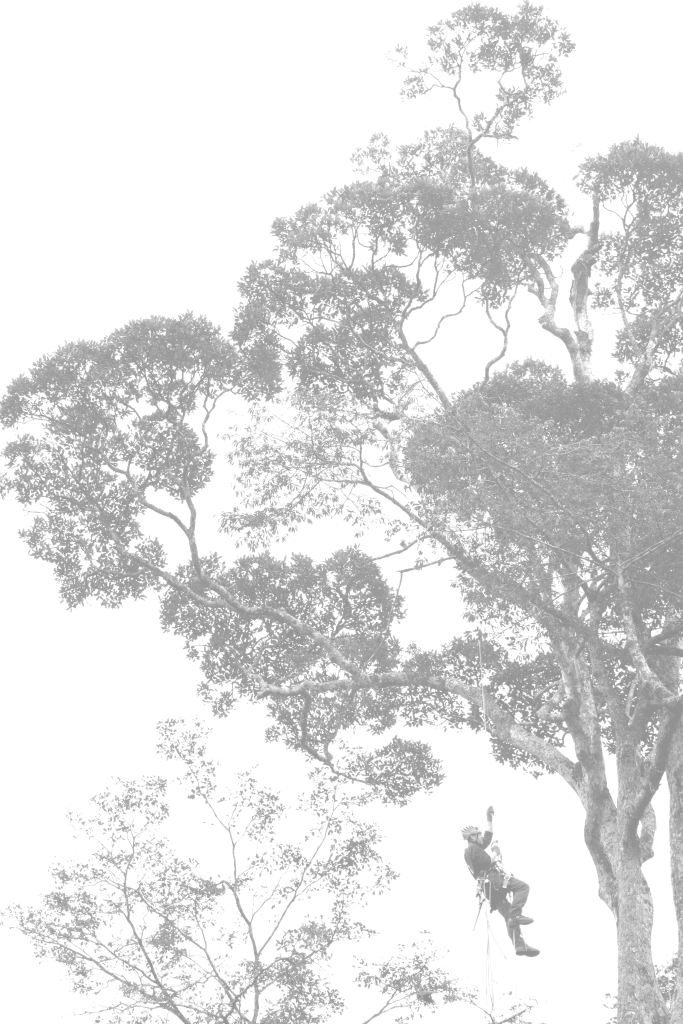
\includegraphics[width=10cm]{Filigrane}
	 \end{textblock}
	\begin{textblock}{140}[0, 1](50, 262)
		\normalfont	Version: \thedate
	\end{textblock}
	\newpage
	~\\ % Print a character or the page will not exist
	\begin{textblock}{140}(40, 40)
		#1
	\end{textblock}
	\begin{textblock}{140}[0,1](40, 270)
		\centering
    \includegraphics[width=5cm]{Logo-Lab}\\ \bigskip
		UMR \'Ecologie des forêts de Guyane\\
		\url{http://www.ecofog.gf}\\[3\baselineskip]
		Les opinions émises par les auteurs sont personnelles et n’engagent ni l’UMR EcoFoG ni ses tutelles.

    \tiny{Photographie en couverture: Hadrien Lalagüe}
	\end{textblock}
	\newpage
}

% PhD / HDR Thesis
%%%%%%%%%%%%%%%%%%%%%%%%%%%%%%%%%%%%%%%%%%%%%%%%%%%%%%%%%%

\usepackage[DocType=PhD, ED=UG, Ets=UG, DIS=ST]{latex/pdgUniv}

\specialty{Écologie}
\defencedate{Novembre 2018}
\lab{UMR EcoFoG, Écologie des Forêts de Guyane}
% ==================
% Setup people like your boss, the jury team and the referees
% - First you need to define how number they will be in each category
%   It is done with the commands \nboss{n}, \nreferee{n} and \njudge{n}.
%   You can define more people in each category than the number given
%   but only the first "\npeople" will be print.
% - Then use the command \makesomeone{<category>}{<number>}{<name>}{<status>}{<other>}
%   where:
%     <category> should be select in ['boss', 'referee', 'judge']
%     <number>   is the rank for printing the person.
%                Only number <= "\npeople" will be printed
%     <name>     First name and las name of the people
%     <status>   Is (s)he a "charg\'e de recher" ou un "professeur d'universit\'e"...
%     <other>    What ever string you want to add (laboratory, jury member place...).
\njudge{6}
\makesomeone{judge}{1}{Olivier Hardy}{Professeur d'Université}{Rapporteur}
\makesomeone{judge}{2}{Prenom NomJury2}{Professeur d'Universite}{Membre du Jury}
\makesomeone{judge}{3}{Eric Marcon}{Chercheur}{Directeur de thèse}
\makesomeone{judge}{4}{Bruno Hérault}{Chercheur}{Co-directeur de thèse}






% End of preamble
%%%%%%%%%%%%%%%%%%%%%%%%%%%%%%%%%%%%%%%%%%%%%%%%%%%%%%%%%%


\begin{document}
\frontmatter

% Title page
%%%%%%%%%%%%%%%%%%%%%%%%%%%%%%%%%%%%%%%%%%%%%%%%%%%%%%%%%%

\MainTitlePage[A Maryse, merci.]

\makeflyleaf
\newpage
~
\newpage




% Before Body
%%%%%%%%%%%%%%%%%%%%%%%%%%%%%%%%%%%%%%%%%%%%%%%%%%%%%%%%%%




% Contents
%%%%%%%%%%%%%%%%%%%%%%%%%%%%%%%%%%%%%%%%%%%%%%%%%%%%%%%%%%

\LargeMargins
{
\hypersetup{linkcolor=}
\setcounter{tocdepth}{3}
\tableofcontents
}


% Body
%%%%%%%%%%%%%%%%%%%%%%%%%%%%%%%%%%%%%%%%%%%%%%%%%%%%%%%%%%

\LargeMargins






















\mainmatter

\chapter*{Remerciements}\label{remerciements}
\addcontentsline{toc}{chapter}{Remerciements}

Pour ce travail et tout ce qu'il a apporté de connaissances,
d'expériences et de rencontres je remercie mes directeurs de thèse Eric
Marcon et Bruno Hérault. Je suis consciente de la chance que j'ai eu
d'avoir été leur étudiante, merci pour vos conseils avisés, votre
patience inébranlable et tout votre soutien. Merci surtout de m'avoir
accordé votre confiance de m'avoir offert ces trois belles années.

Merci aux rapporteurs de ma thèse et aux membres du jury d'avoir accepté
de consacrer leur temps à la relecture et à l'évaluation de mon travail.

Merci au Labex Ceba qui a financé ma thèse et largement contribué au
cadre scientifique qui l'a accompagnée. Merci au Cirad et à tous ceux
qui ont travaillé et travaillent encore à Paracou pour faire de ce coin
de paradis une telle source de connaissances. A Pascal, Michel,
Martinus, Frits, Petrus, Onoefé, Richard, Lindon, Aurélie, Géraldine et
tous ceux qui ont permis l'existence de Paracou, merci pour votre
travail titanesque. En particulier, merci Pascal pour ta patience et ta
gentillesse, j'attends avec impatience de retourner sur le terrain.

Merci également aux membres de mon comité de thèse, Adeline Fayolle,
Sandrine Pavoine, Stéphane Guitet, Bart Haegeman, et Chris Baraloto pour
leurs conseils avisés et leurs encouragements.

Enfin, à tous ceux qui ont rendu ces trois années aussi incroyables, les
mots sont difficiles à trouver mais les faits parlent d'eux-mêmes: j'ai
découvert la Guyane, je suis revenue, je suis restée et maintenant je ne
veux plus en partir. Pa Moli!

\chapter{Introduction générale}\label{introduction-generale}

Les forêts couvrent 30\% de la surface terrestre et assurent de nombreux
biens et services environnementaux, économiques et sociaux
indispensables à l'équilibre planétaire. Malgré leur importance les
forêts sont aujourd'hui extrêmement menacées dans le contexte de
changements globaux actuel.

\section{Les forêts tropicales, au coeur des enjeux
actuels}\label{les-forets-tropicales-au-coeur-des-enjeux-actuels}

Par ``forêt'' ou ``ecosystème forestier'' on entend les assemblages de
plantes, animaux et microorganismes au sein de leur environnement
définissant une unité fonctionnelle. Les arbres sont les composants
essentiels de ces écosystèmes forestiers \autocite{FRA2000}. Les forêts
sont les régions les moins anthropisées du globe et portent de forts
enjeux de conservation en accueillant la diversité animale et végétale
et les taux d'endémisme les plus importants du globe
\autocites{Myers2000}{Mittermeier2003}.

A l'échelle locale, les forêts entretiennent les cycles de l'eau et des
nutriments (azote, phosphore, etc), et régulent le climat et la
fertilité des sols \autocites{Malhi2008}{Isbell2017}. A l'échelle
globale ce sont des éléments centraux dans la régulation des gaz à effet
de serre (\emph{GES}), en tant que puits de carbone de 1.1 ± 0.8
PgC.yr\textsuperscript{--1} qui compensent une partie des émissions de
GES, mais également en tant que sources potentielles lorsque leur
dégradation libère le carbone stocké dans leur biomasse
\autocites{Pan2011}{Roy2017}.

Les forêts assurent directement la subsistance de 500 millions de
personnes en tant que source de nourriture (par la chasse et la collecte
de produits forestiers non ligneux comestibles), d'eau, de matériaux de
construction, et d'énergie (par l'utilisation du bois de chauffage et de
cuisson). Elles sont de plus indispensables au bien-être des populations
et possèdent d'importantes dimensions culturelle, spirituelle et
patrimoniale \autocites{FRA2015}{Tilman2014}. Enfin, l'exploitation
forestière correspond à de forts enjeux économiques: elle représente
\textasciitilde{} 1\% du PIB mondial, une part importante de l'emploi et
reste l'une des principales sources d'énergie
\autocites{CBDdiversity2011}{FAO2014}.

Indispensables et irremplaçables, les forêts sont néanmoins dégradées ou
disparaissent à une vitesse croissante: entre 2013 et 2015 leur surface
globale a diminué de 3\% \autocite{FAO2009}. Elles subissent de fortes
pressions anthropiques allant des changements d'usage des terres via
déboisement pour l'élevage ou l'agriculture, à l'exploitation du bois
légale ou illégale, la chasse ou l'introduction d'espèces invasives.
Elles subissent également les changements climatiques globaux qui
augmentent la fréquence des événements extrêmes tels que les
sécheresses, les incendies, ou les inondations
\autocite{Pachauri2014}.\newline

Dans ce contexte les forêts tropicales, représentant 19.6 million de
km², sont les régions à la fois les plus menacées et celles aux enjeux
les plus importants \autocite{Barlow2018}. Les forêts tropciales
accueillent la diversité biologique la plus élevée au monde et sont les
plus grandes forêts n'ayant jamais connu de forte perturbation
anthropique \autocites{Gentry1988}{FAO2011}. Historiquement peu
peuplées, ces régions connaissent cependant une croissance démographique
moyenne de près de 1,4\% par an qui s'accompagne d'un développement
économique proportionnel \autocite{Asner2009}. L'impact de ces pressions
anthropiques est de plus exacerbé par le contexte économique de
nombreuses zones tropicales, où les investissements, les politiques de
conservation et les capacités de recherche et de développement sont
moindres. Les impacts de ces pressions locales s'ajoutent aux
changements globaux et entraînent des modifications importantes des
écosystèmes, allant souvent vers une dminution de la diversité
biologique. Ces changements correspondent à la disparition locales
d'espèces qui peut entraîner des changements écosystémiques plus
profonds selon le rôle des espèces dans la communautés. Ces
disparitions, qui constituent l'érosion actuelle de la biodiversité,
sont telles qu'elles ont déjà été qualifiées de ``sixième extinction de
l'ère moderne'' \autocites{Vitousek1997}{Cardinale2012}.

Une prise de conscience globale de la situation globale a été entérinée
par la conférence des nations unies sur l'environnement et le
développement à Rio en 1992. De nombreux engagements politiques ont été
pris vis à vis de la surveillance et de la conservation de la
biodiversité et de la préservation du fonctionnement des forêts mais les
menaces persistent voire grandissent malgré tout
\autocites{Summit1992}{Schlaepfer2000}{Dirzo2003a}{Morales-Hidalgo2015}.
Ces engagement doivent être maintenus et améliorés aujourd'hui.
Plusieurs approches ont été adoptées pour assurer la conservation de la
biodiversité. La première s'appuie sur la création d'aires protégées, de
plus en plus étendues aujourd'hui, mais dont les surfaces demeurent
insuffisantes pour pallier l'érosion globale de la biodiversité
\autocite{Sist2015}. La seconde approche propose d'intégrer à la gestion
des écosystèmes les enjeux à la fois environnementaux, économiques et
humains. Cela se traduit par l'intégration des services écosystémiques
comme enjeu de gestion grâce à leur valorisation économique, via la
création de de systèmes de paiement, de programmes comme le REDD+ ou de
divers labels \autocites{Agrawal2011}{Barlow2018}. Cette approche se
traduit également par la mise en place de modes de gestion fondés sur
les interactions entre nature et société, via par exemple la gestion
communautaire des forêts impliquant les populations locales
\autocite{Liu2015}.

\section{Exploitation et conservation des forêts
tropicales}\label{exploitation-et-conservation-des-forets-tropicales}

L'une des approches les plus intuitives et courantes pour la
conservation des forêts tropicales est la désignation d'aires protégées
exemptes de toute activité anthropique. Cette approche seule ne suffit
cependant pas pour maintenir l'incroyable biodiversité de ces forêts et
leur fonctionnement complexe \autocite{Sist2015}. Pour cela
l'exploitation forestière joue aujourd'hui un rôle central en permettant
à la fois le maintien du fonctionement des forêts et un développement
économique et social, sous réserve d'une gestion adéquate.

L'exploitation sélective est l'exploitation de quelques espèces cibles
dont les individus exploités sont désignés à l'avance. Elle concerne
environ 20\% de la surface des forêts tropicales et représente 12\% de
la production mondiale de bois d'oeuvre \autocite{Martin2015}. Cette
exploitation crée des trouées éparses et nécessite l'ouverture d'un
réseau important de dessertes modifiant la structure de la canopée.
L'exploitation sélective peut impacter le fontionnement des communautés
mais reste néanmoins bien moins préjudiciable que de nombreuses autres
activités anthropiques. Bien gérée, l'exploitation sélective représente
un potentiel de conservation important car elle allie développement
économique et préservation du fonctionnement des forêts, mais peut
également peut avoir des impacts négatifs comme par exemple des
changements de composition et de diversité, voire l'extinction locale
d'espèces \autocite{Gibson2011}. L'impact de l'exploitation sélective en
forêt tropicale dépendra des pratiques de gestion. ces pratiques sont
définies principalement par le diamètre minimum de coupe et par le temps
de récupération après exploitation \autocite{Sist2015}, et sont
aujourd'hui essentiellement calibrées en vue de la reconstitution du
stock de bois d'oeuvre. Elles intègrent cependant de plus en plus des
enjeux de conservation en visant le maintien de la production sans
entraîner de préjudice à l'intégrité et la productivité des forêts, ni
de dommages environnementaux ou sociaux \autocite{ITTO2005}. La gestion
durable des forêts, définie par l' ITTO (\emph{International Tropical
Timber Organization}), doit ainsi permettre la restauration de la
diversité en espèces et du fonctionnement de l'écosystème après
exploitation. Dans ce contexte, toute réflexion sur la durabilité et
l'amélioration de la gestion sylvicole nécessite de bien connaître
l'impact de l'exploitation sur la diversité et la composition des forêts
.

\section{Diversité et assemblage des
communautés}\label{diversite-et-assemblage-des-communautes}

Comprendre et anticiper la réponse aux perturbations des forêts
tropicales passe par l'étude des communautés d'arbres, qui en sont les
éléments principaux, et en particulier par leur diversité et leur
composition. La diversité des communautés d'arbres reflète celle des
autres groupes floristiques et faunistiques et détermine largement le
fonctionnement des communautés \autocite{Guitet2017}. Individuellement,
chaque espèce a une valeur intrinsèque pour le patrimoine naturel global
et en fonction de ses caractéristiques biologiques peut avoir un rôle
clé dans la communauté, comme c'est la cas pour les espèces \emph{clé de
voûte} \autocites{Jones1994}{Power1996}{Gardner2007}. A l'échelle de la
communauté la diversité et la composition des communautés détermine les
interactions entre individus et avec l'environnement, et déterminent don
le fonctionnement et la productivité des écosystèmes
\autocite{Begon2006}. La diversité détermine également la stabilité et
la résilience des communautés en atténuant l'impact des maladies, des
espèces invasives et des variations environnementales
\autocite{Elmqvist2003}. Toute perturbation ou changement susceptible de
modifier la biodiversité et la composition des communautés impacte donc
le fonctionnement des écosystèmes, mais le détail de ces impacts et de
leurs conséquences reste mal connu.

\subsection{Succession, mortalité et recrutement: supports de la
trajectoire des
communautés}\label{succession-mortalite-et-recrutement-supports-de-la-trajectoire-des-communautes}

Une perturbation correspond à des changements de l'environnement
biotique (interactions entre individus) et abiotique (ensoleillement,
flux d'eau, de nutriments et de matière). La réponse des communautés aux
perturbations a été décrite comme une succession temporelle de processus
écologiques consécutifs à ces changements environnementaux
\autocite{Clements1916}. Les modèles de succession identifiés impliquent
dans un premier temps le recrutement d'espèces pionnières, meilleures
acquisitrices des ressources rendues disponibles après perturbation.
Dans un deuxième temps la croissance de ces premiers recrutés diminue la
disponibilité en ressources et augmente la compétition, excluant du
recrutement les espèces les moins compétitrices. Les pionnières
recrutées en premier lieu deviennent alors sénescentes ou exclues par la
compétition, et sont petit à petit remplacées par les espèces de
succession tardive qui correspondent en forêt tropicale à des espèces de
croissance lente mais à longue durée de vie.

Ce modèle de succession correspond à différentes combinaisons de
processus de mortalité (disparition) et de recrutement (apparition)
d'espèces dans la communauté et restaure ainsi de façon déterministe une
communauté typique de succession tardive \autocite{Denslow2000}. Le
recrutement est ainsi un élément clé de la réponse des communautés aux
perturbations. Le recrutement regroupe l'ensemble des processus de
production, de dissémination et de germination des graines, et de survie
et de croissance des plantules jusqu'à un seuil de recrutement. Ce seuil
est un diamètre minimum représentatif de la taille et de la biomasse de
l'arbre à partir duquel l'individu est considéré comme assez développé
pour participer significativement au fonctionnement de l'écosystème et
est intégré aux inventaires. Les nombreux processus écologiques qui
régulent les différentes étapes du recrutement sont donc des
déterminants majeurs de la réponse des communautés aux perturbations
\autocites{Denslow1980}{Schnitzer2001}{Asner2004}.

\subsection{Les règles d'assemblage des
communautés}\label{les-regles-dassemblage-des-communautes}

La réponse des communautés aux perturbations résulte d'un ensemble de
processus d'assemblage et de maintien des espèces. Plusieurs hypothèses
quant à ce sprocessus sont débattues aujourd'hui, notamment vis à vis de
l'importance des processus stochastiques et déterministes. Les processus
déterministes sélectionnent les espèces de la communauté sur la base de
leurs caractéristiques biologiques, en fonction de leurs performance
dans l'environnement biotique et abiotique \autocite{Molino2001}. Les
processus stochastiques, qui relèvent de la théorie neutre, supposent un
assemblage aléatoire des espèces dépendant uniquement de l'histoire de
la communauté et des limitations physique de dispersion ou de croissance
(barrière à la dispersion, ordre d'arrivée des espèces)
\ref{fig:AssemblyRules} \autocite{Hubbell2001}.

Le débat quant au rôle respectif des processus stochastiques et
déterministes est matérialisé par la controverse sur la théorie des
perturbations intermédiaires (\emph{Intermediaite Disturbance
Hypothesis}, \emph{IDH} en anglais). Cette théorie suppose la
prépondérance de processus déterministes d'exclusion compétitive et
prédit une diversité maximale pour des régimes de perturbation réguliers
et d'intensité moyenne évitant la dominance de quelques espèces
\autocite{Molino2001}. Un tel régime de perturbations intermédaires
premet en effet une variabilité des conditions environnementales qui
permet à un large panel d'espèces de s'installer lorsque les conditions
environnementales leur deviennent favorables, puis de persister dans la
communauté. Au delà d'un seuil d'intensité de perturbation en revanche
un trop grand nombre d'espèces sont exclues et les quelques espèces
favorisées deviennent dominantes, si bien que la diversitédiminue
\autocites{Chesson2000}{Kariuki2006a}{Berry2008a}.

A l'inverse la théorie neutre suppose que les espèces sont équivalentes
et que leur abondance ne dépend pas de leurs caractéritiques
biologiques. Les espèces favorisées suite aux perturbations seraient
alors variables, l'abondance des espèces dépendrait uniquement de
processus aléatoires de dispersion, de croissance et de survie résultant
en un assemblage stochastique des communautés \autocite{Hubbell2001}.

Bien que débattues les hypothèses déterministe et stochastique ne sont
pas incompatibles et peuvent prédire la structure des communautés à
différentes échelles et pour différents niveaux de richesse. Il est
vraisemblable que les règles d'assemblage des communautés soient une
combinaison variable de processus déterministes et stochastiques, et la
question se pose alors des facteurs qui déterminent ces combinaisons
\autocite{Chave2004}.

\section{Comment mesurer la diversité biologique
?}\label{comment-mesurer-la-diversite-biologique}

Mesurer la diversité des communautés, déterminante du fonctionnement et
du maintien des écosystèmes, est essentiel pour prédire et gérer
l'avenir des forêts. La diversité est cependant une notion complexe qui
englobe la diversité génétique et phénotypique des individus, et la
variabilité de leurs assemblages \autocite{Loreau2005}. La biodiversité,
souvent réduite à la notion de richesse spécifique, prend donc également
en compte des aspects de richesse, d'équitabilité d'abondance, de
similarité entre espèces. En plus de quantifier la diversité des
communautés, ces différents aspects permettent d'appréhender les
mécanismes écologiques régissant les écosystèmes et leurs dynamiques
spatiales et temporelles \autocites{Purvis2000}{Loreau2005}.

\subsection{Composition et
dissimilarité}\label{composition-et-dissimilarite}

Comparer des communautés ou suivre leur évolution au cours du temps
implique dans un premier temps de comparer leur composition et de
quantifier le turnover des espèces. De nombreuses mesures permettent
d'estimer ce turnover, prenant en compte ou non l'abondance des espèces
\autocite{Podani2013}. Dans la suite de cette thèse nous avons choisi de
mesurer le taux de remplacement d'abondance, ou similarité de
Bray-Curtis, qui estime dans quelle mesure une communauté est le
sous-ensemble d'une autre. Si le turnover des espèces entre deux
communautés est faible, l'une d'elles sera comme le sous-échantillonnage
de l'autre, comme si elle en avait été tirée au hasard. La similarité de
Bray-Curtis est la somme des abondances d'une communauté qui
correspondent à une espèce différente dans l'autre communauté,
normalisée ensuite par l'abondance totale partagée entre les deux
communautés \eqref{eq:formNestedness}.

\begin{equation}
T_{ab}=\frac{\sum_{i=1}^{n}|x_i^a - x_i^b| - \bigg| \sum_{i=1}^{n}{x_i^a} - \sum_{i=1}^{n}{x_i^b} \bigg|}{\sum_{i=1}^{n}\max{\left( x_i^a;x_i^b \right)}}
\label{eq:formNestedness}
\end{equation}

\subsection{Assemblage et structure des
communautés}\label{assemblage-et-structure-des-communautes}

Outre la composition en espèce l'étude de la biodiversité est l'étude de
la diversité des communautés, comprenant la richesse et la distribution
d'abondance. Une communauté est constituée d'espèces aux effectifs
différents: certaines sont très abondantes, d'autres communes et
d'autres encore, souvent la majorité, sont rares. La façon la plus
simple et immédiate de décrire une communauté est de donner les
proportions d'espèces abondantes rapport aux espèces communes ou rares,
représentées par la distribution d'abondance de la communauté. Cette
distribution d'abondance est régie par des lois écologiques et,
moyennant quelque variations, prend invariablement la forme d'une courbe
en creux \ref{fig:AbdDist} \autocite{McGill2007}.

\begin{figure*}

{\centering 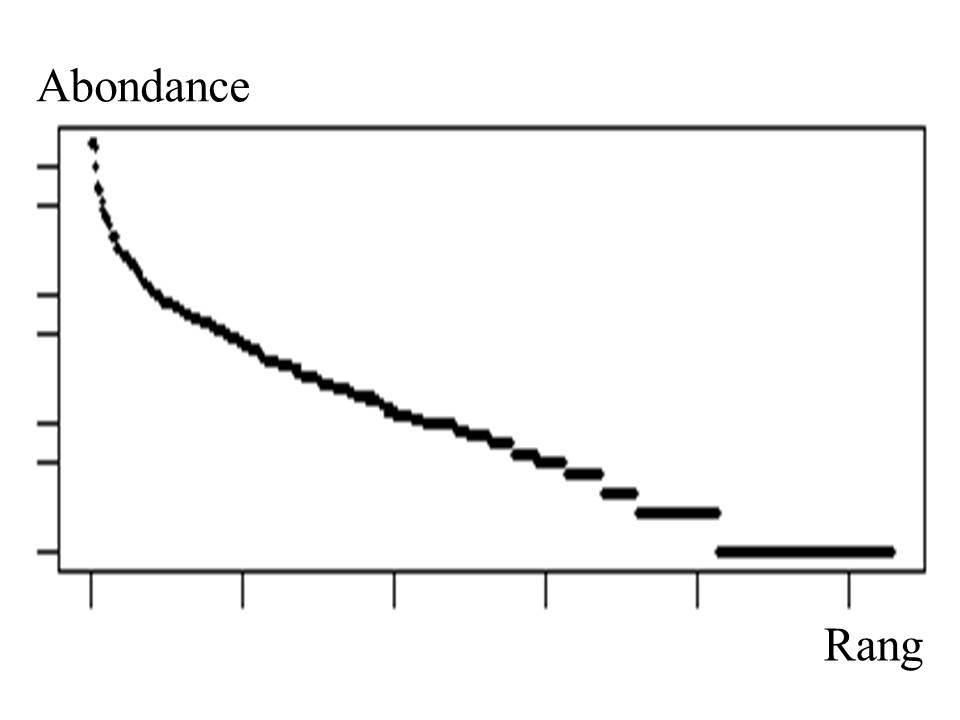
\includegraphics[width=0.6\linewidth]{ExternalFig/SpeciesAbdDist} 

}

\caption{Exemple de distribution d'abondance pour une communauté d'arbres en forêt tropicale humide}\label{fig:AbdDist}
\end{figure*}

Cette uniformité des distributions d'abondance a motivé le développement
de modèles proposant des relations mathématiques entre le nombre
d'espèces et leur abondance. Ces modèles reflètent le lien entre
l'importance d'une espèce dans la communauté et la quantité de
ressources qu'elle mobilise pour son développement: plus une espèce est
compétitive, plus elle sera abondante. Ce lien s'établit vis à vis de la
ressource limitante, qui peut être la lumière, l'eau, les nutriments,
l'espace, etc \autocites{Silvertown2004}{terSteege2006}. Prédire une
distribution d'abondance revient à prédire la répartition de la
ressource limitante entre espèces de la communauté. De nombreux modèles
prédictifs ont été proposés: des modèles statistiques divisant
aléatoirement la ressource selon une loi de propabilité donnant les
effectifs de chaque espèce, aux modèles mécanistes divisant la resource
selon une formule prédéterminée comme par exemple selon une division
systématique de la ressource restante
\autocites{Fisher1943}{Motomura1932}{Tokeshi1993}{Magurran1988}.

Ces modèles testés pour de nombreuses communautés ont montré représenter
correctement les communautés réelles et pouvoir révéler les règles
écologiques régissant l'assemblage des espèces. Ce sont donc des outils
adéquats pour comparer les communautés et en interpréter les
différences. Manipuler une distribution d'abondance est cependant
compliqué car il s'agit d'une représentation en deux dimensions qui ne
permet pas de quantifier les différences entre communautés. En revanche,
les paramètres de ces distributions et des modèle proposés permettent de
résumer de façon quantifiable les caractéristiques des distributions
d'abondance. Ces différents paramètres, les indices de diversité,
correspondent au nombre d'espèces, à la forme des distributions, ou
encore à l'homogénéité des abondances.

\subsection{Les composantes de la
diversité}\label{les-composantes-de-la-diversite}

La diversité est souvent assimilée à la richesse en espèce, qui
correspond au nombre d'espèces qui constituent la communauté. La
richesse ne tient cependant pas compte de l'abondance des espèces qui
est pourtant un paramètre essentiel, une espèce dominante n'apportant
pas la même contribution à l'écosystème qu'une espèce rare. Une
communauté dominée par une ou deux espèces très abondantes sera
intuitivement moins diverse qu'une communauté avec le même nombre
d'espèces mais ond les abondances sont équivalentes. L'homogeneité des
abondances dans une population est l'\emph{équitabilité}, et elle peut
être bien plus révélatrice du fonctionnement des écosystèmes que la
richesse ou la composition. Selon l'hypothèse du ratio de biomasse en
effet, le fonctionnement des écosystèmes repose bien plus sur les
caractéristiques des espèces dominantes que sur celles des espèces
rares. Les espèces rares n'ont pas d'influence si elles sont
transitoires ou alors une influence qu'à long terme en tant que futures
dominantes potentielles \autocite{Grime1998}.

La richesse, simplement le nombre d'espèces recensées, et
l'équitabilité, la régularité de distribution d'abondance des espèces,
sont donc les deux composantes de la diversité taxonomique d'une
communauté \ref{fig:RichEqu} \autocites{Whittaker1965}{Magurran2004}.

\begin{figure*}

{\centering 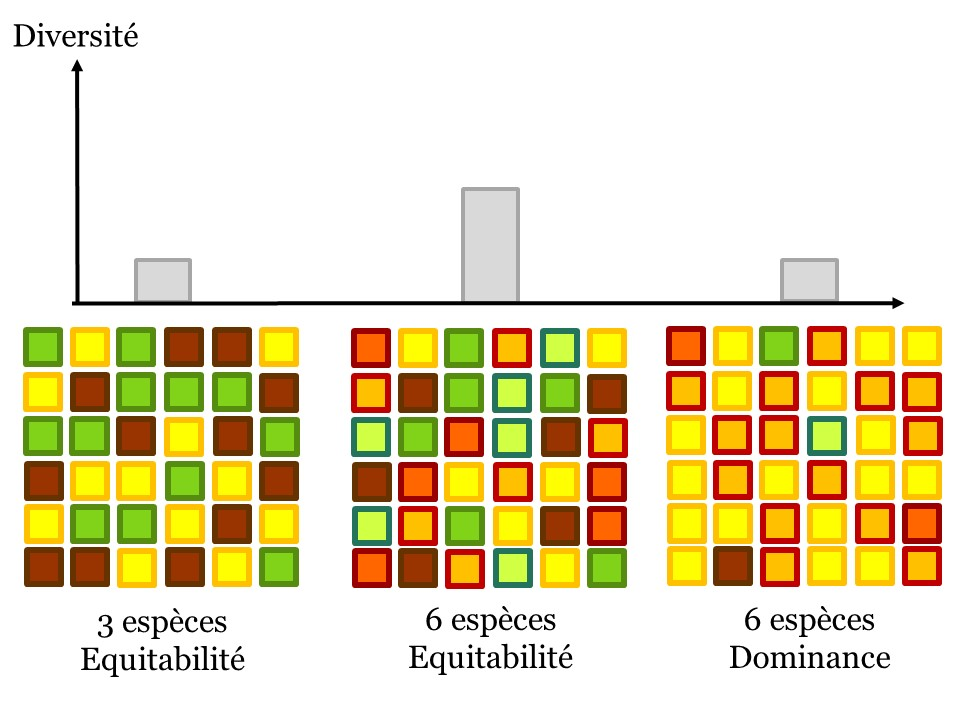
\includegraphics[width=0.6\linewidth]{ExternalFig/Fig_RichnessEquitability} 

}

\caption{Les deux composantes de la diversité taxonomique: richesse (nombre d'espèces) et équitabilité (homogeneité de répartition)}\label{fig:RichEqu}
\end{figure*}

Estimer la diversité d'une communauté ne revient donc pas à une mesure
unique mais à un ensemble de mesures combinant différemment les
composantes de la diversité. Plusieurs familles d'indices de diversité
ont été développées: une famille correspond aux déclinaisons d'une même
formule accordant un poids variable aux différentes composantes de la
diversité. La famille des indices de diversité de Réyni par exemple,
judicieuse pour l'étude des communautés végétales, rassemble les indices
mesurés selon l'équation \eqref{eq:formHCDT} modulée par un paramètre
\emph{q} appelé ``ordre de diversité''. L'ordre de diversité q
correspond au poids donné aux espèces rares par rapport aux espèces
abondantes, plus l'ordre de diversité est élevé, plus les espèces rares
sont négligées par rapport aux espèces abondantes \autocite{Mendes2008}.

\begin{equation}
{^{q}H=\frac{1}{q-1}\Bigg(1-\displaystyle\sum_{s=1}^{S}p^q_s\Bigg) }
\label{eq:formHCDT}
\end{equation}

Dans cette famille d'indices de diversité se retrouvent les indices les
plus utilisés dans la littérature. A l'ordre 0 chaque espèce contribue
de la même façon à la mesure, ce qui correspond à la richesse
spécifique. A l'ordre 1 la richesse et équitabilité sont également
prises en compte, ce qui correspond à l'indice de Shannon. Enfin à
l'ordre 2 les espèces rares sont presque négligées,ce qui correspond à
l'indice de Simpson (parfois appelé ``diversité en espèces abondantes'')
\autocites{Shannon1948}{Simpson1949}{Patil1982}{Tothmeresz1995}. Tels
quels, les indices de Réyni sont mathématiquement corrects et
représentatifs des différentes composantes de la diversité, mais ne
donnent pas une mesure intelligible permettant de comparer facilement
différentes communautés. Les indices de diversité doivent être traduits
en \emph{nombre équivalent d'espèces} qui correspond au nombre d'espèces
qu'aurait la communauté étudiée si toutes les espèces avaient la même
abondance. Ce nombre équivalent d'espèces, ou \emph{nombre de Hill}, est
obtenu par transformation des valeurs obtenues selon une exponentielle à
base q \autocite{Hill1973}.

Les mesures de diversité utilisées dans la suite de ce travail sont donc
la traduction intelligible en nombre équivalent d'espèces d'un panel
d'indices combinant richesse et équitabilité de différentes façons pour
capter toute structure de diversité.

\subsection{Résolution du biais
d'échantillonnage}\label{resolution-du-biais-dechantillonnage}

En pratique aucun inventaire n'est exhaustif et l'étude de la diversité
se heurte aux biais d'échantillonnage qui sous-estiment la richesse et
faussent l'abondance des espèces. Corriger ces biais nécessite d'estimer
les abondances réelles à partir des observations et des relations
mathématiques reliant les abondances des différentes espèces. La
première méthode développée correspond à la formule des fréquences de
Turing \autocite{Good1953} où l'abondance réelle *\alpha\_v* d'une
espèce observée \emph{v} fois dans un échantillonnage de \emph{n}
individus dépend du nombre d'espèces observées également \emph{v} fois
et du nombre d'espèces observées \emph{v+1} fois
@ref\{eq=formGoodTuring\}:

\begin{equation}
\alpha_v=\frac{\big(v+1\big)}{n}\frac{s^n_{v+1}}{s^n_v}
\label{eq:formGoodTuring}
\end{equation}

Les singletons (espèces observées une seule fois) et les doubletons
(espèces observées deux fois) sont ici particulièrement intéressants car
il permettent d'estimer le nombre \emph{s\^{}n\_0} d'espèces manquées
observées zéro fois (\(s^n_0=\frac{s^n_1}{n}\)) et donc de corriger le
biais d'échantillonnage de la richesse.

De nombreuses méthodes ont repris cette relation en y intégrant
notamment la notion de \emph{taux de couverture} qui quantifie l'effort
d'échantillonnage d'un inventaire et permet de savoir quelle proportion
de la communauté a été échantillonnée \autocite{Dauby2012}. La
correction la plus adéquate a été déterminée pour chaque taux de
couverture et les estimateurs de la diversité sont aujourd'hui très
fiables \autocites{Chao2015}{Marcon2015b}.

\subsection{Diversité fonctionnelle}\label{diversite-fonctionnelle}

Les mesures de diversité décrites précédemment, appelées diversité
neutre, considèrent toutes les espèces de la même façon quelles que
soient leurs caractéristiques biologiques ou phylogénétiques. Ces
caractéristiques peuvent cependant facilement intégrer les mesures de
diversité au même titre que la richesse et l'équitabilité, en passant
pas la similarité entre espèces. Une communauté sera d'autant plus
diverse que les espèces qui la constituent sont différentes. Pour des
communautés végétales la diversité phylogénétique considère les
distances entre espèces dans un arbre phylogénétique et la diversité
fonctionnelle considère leurs différences morphologiques ou
physiologiques \ref{fig:RichEquSim}.

\begin{figure*}

{\centering 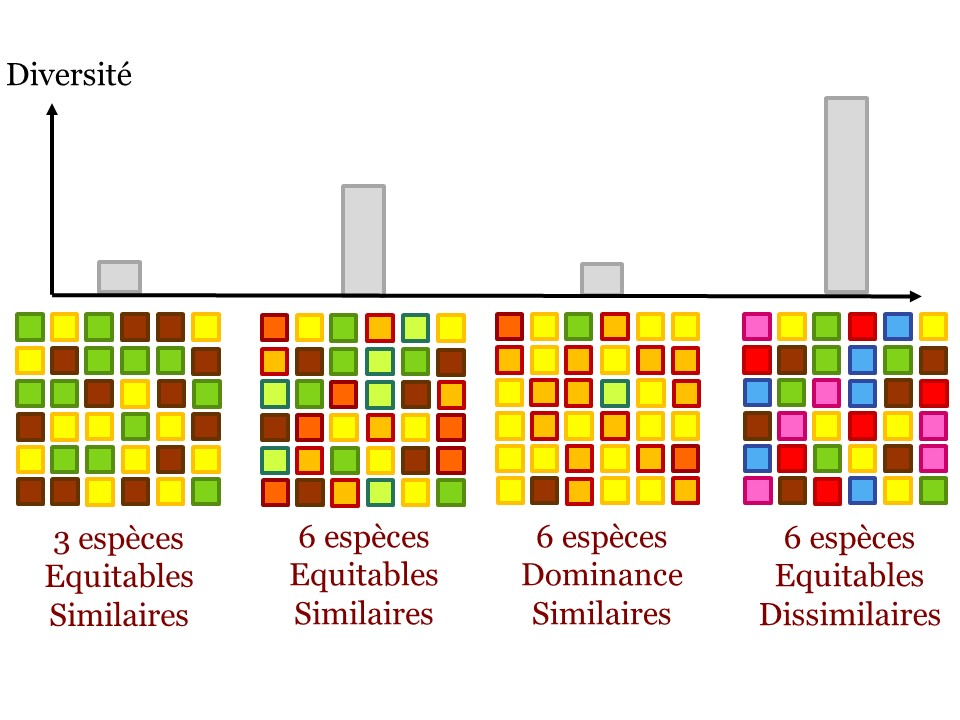
\includegraphics[width=0.6\linewidth]{ExternalFig/Fig_RichnessEquitabilitySimilarity} 

}

\caption{Troisième composante de la diversité: la similarité entre espèces basée sur des distances phylogénétiques ou taxonomiques}\label{fig:RichEquSim}
\end{figure*}

La similarité au sein d'une communauté est intégrée sous la forme d'une
matrice de distances entre espèces calculée sur la base de leur
phylogénie ou de leurs traits fonctionnels. Les traits fonctionnels sont
les caractéristiques morphologiques, physiologiques et phénologiques des
espèces, ils déterminent le fonctionnement des individus, leur
performance en termes de croissance et de survie, et leurs interactions
avec l'environnement \autocite{Violle2007b}. L'approche fonctionnelle
qui décrivt les espèces et les individus selon leurs caractéristiques
biologiques a été largement adoptée en écologie. Elle permet d'une part
de réduire la dimensionnalité des communautés, indispensable pour
l'étude d'écosystèmes aussi riches que les forêts tropicales, et de
comparer les communautés quelle que soit leur composition en espèces
\autocites{Begon2006}{Scheiter2013}{Mouillot2013a}{Sakschewski2016}.
D'autre part l'approche fonctionnelle permet d'appréhender directement
la diversité des communautés et leur fonctionnement, la composition et
diversité fonctionnelle étant interprétables en termes d'utilisation des
ressources et de flux de matière et d'énergie. Enfin, cette approche
appréhende la signature fonctionnelle des perturbations et permet
d'identifier et de quantifier les processus écologiques déterminant la
réponse des communautés aux perturbations \autocite{Funk2017}.
Spécifiquement, l'approche fonctionnelle appréhende l'importance des
processus déterministes dépendant par les caractéristiques biologiques
des espèces. L'exclusion d'espèces non adaptées à l'environnement se
traduira par une aggrégation de la communauté dans l'espace des traits
fonctionnels et une diminution de sa diversité fonctionnelle, tandis que
l'exclusion compétitive limitant les similarité entre espèces se
traduira par une dispersion des traits fonctionnels de la communauté et
une augmentation de la diversité fonctionnelle
\autocites{McGill2006}{Kunstler2012}.

L'approche fonctionnelle nécessite de choisir judicieusement les traits
intégrés aux indices de diversité. Une vaste littérature a permis
d'identifier les traits clés représentatifs de l'écologie et de la
croissance des espèces et de leur influence sur le fonctionnement de
l'écosystème \autocite{Reich2014}. Les traits foliaires tout d'abord,
déterminant la stratégie d'acquisition et d'allocation des resources
lumineuses, définissent un ``spectre économique foliaire''. Ce spectre
oppose les espèces à larges feuilles fines ayant une forte capacité
photosynthétique et donc une acquisition rapide des resources, aux
espèces à petites feuilles coriaces et résistantes. Un gradient
similaire s'applique aux traits racinaires et aux propriétés du bois,
opposant les espèces aux tissus légers et à croissance rapide, aux
espèces aux tissus denses mobilisant plus de ressources
\autocites{Chave2009}{Valverde-Barrantes2017}. Les stratégies
d'acquisition déterminent la stratégie de croissance des espèces: tandis
que les ``acquisitives'' auront une croissance rapide et une courte
durée de vie, les ``conservatives'' auront une croissance plus lente
mais une meilleure résistance aux conditions environnementales
éprouvantes \autocites{Reich1997}{Wright2004}. A ces traits fonctionnels
mesurables à l'échelle de l'individus s'ajoutent des \emph{traits
d'histoire de vie} mesurables à l'échelle de l'espèce. Parmi ces traits
la masse des graines et la hauteur moyenne maximale des arbres à l'âge
adulte sont particulièrement représentatifs des stratégies de
croissance, de survie et de reproduction
\autocites{Westoby1998}{Herault2011}. L'engouement récent de l'écologie
pour l'approche fonctionnelle a de plus permis la création de bases de
données fonctionnelles conséquentes et standardisées qui rendent
possibles l'approche fonctionnelle à l'échelle des communautés
\autocites{Kattge2011}{Perez-Harguindeguy2013} \footnote{\url{http://www.ecofog.gf/Bridge/}}

L'approche fonctionnelle considère la diversité des communautés mais
également leur composition fonctionnelle mesurable par les valeurs
moyennes de traits pondérées par l'abondance des espèces
(\emph{Community Weighted Means, CWM} en anglais). L'abondance des
caractéristiques fonctionnelles détermine à la fois le fonctionnement et
la résilience des communautés. D'après la théorie du ``ratio de
biomasse'' \autocite{Grime1998}, le rôle d'un individu dans l'écosystème
dépend de la fraction de biomasse qu'il représente et le fonctionnement
des communautés repose sur les espèces dominantes tandis que les espèces
rares ont peu d'influence.

Par ailleurs la répartition d'abondance des traits fonctionnels amène à
la notion de redondance fonctionnelle qui quantifie le nombre d'espèces
partageant les mêmes valeurs de traits. La redondance fonctionnelle,
souvent élevée en forêt tropicale, permet aux communautés de perdre des
espèces sans nécessairement voir disparaître leur rôle dans
l'écosystème: la redondance détermine en partie la résilience des
communautés et atténue l'impact des perturbations. La redondance
fonctionnelle d'une communauté se mesure dans l'espace fonctionnel à
partir de la densité de probabilité de traits (\emph{Traits Density
Probability, TDP} en anglais) de chaque espèce \autocite{Carmona2016}.
Les densités des espèces d'une communauté pondérées par leur abondance
sont additionnées pour donner la redondance fonctionnelle sur l'ensemble
de l'espace fonctionnel ou sur un espace restreint
\ref{fig:RedundancyMethod}.

\begin{figure*}

{\centering 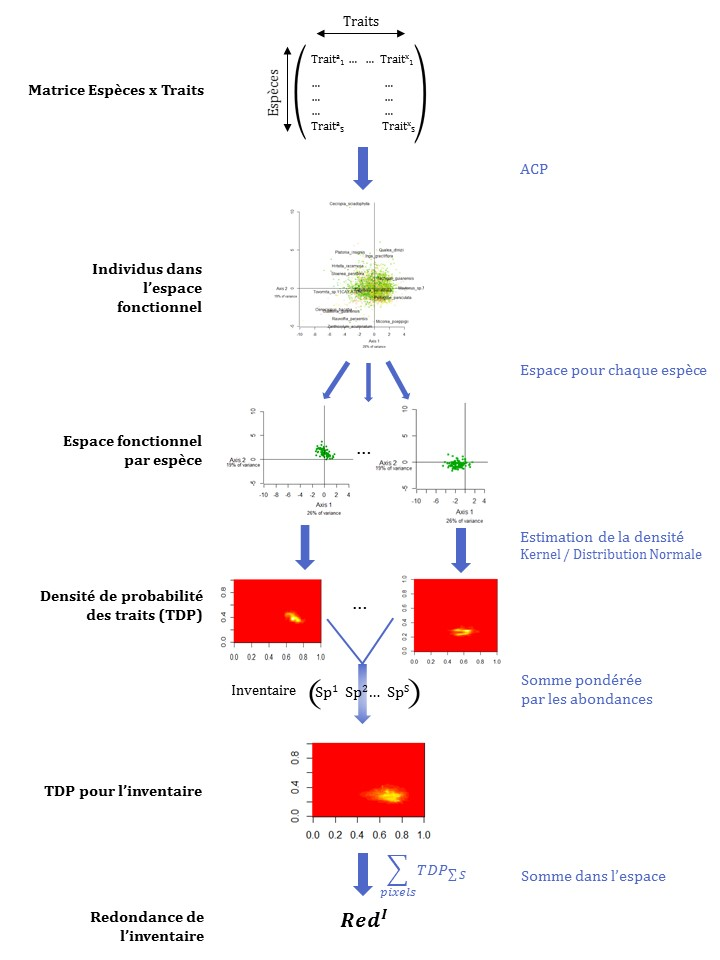
\includegraphics[width=1\linewidth]{ExternalFig/Fig_MesureRedondance} 

}

\caption{La redondance fonctionnelle est la somme des chevauchement entre espèces dans l'espace fonctionnel. Les individus de la base de données fonctionnelle sont représentés dans un espace à 2 dimensions grâce à une analyse en composantes principales (ACP). Une estimation par noyau estime ensuite la densité de probabilité des traits (TDP) de chaque espèce. La somme de ces densités pondérées par l'abondance des espèces donne enfin la redondance fonctionnelle de la communauté, interprétable comme le nombre d'espèces qui peuvent disparaître sans diminuer l'espace fonctionnel de la communauté.}\label{fig:RedundancyMethod}
\end{figure*}

\section{La Guyane Française et l'exemple de la station de
Paracou}\label{la-guyane-francaise-et-lexemple-de-la-station-de-paracou}

Le bassin Amazonien est région de forêt tropicale humide où la
biodiversité est la plus élevée \autocite{Gentry1988}. La Guyane
française est une région de 83 846 km\textsuperscript{2} au Nord-Est du
bassin Amazonien entre le Suriname et le Brésil recouverte à 95\% de
forêt.

\subsection{Le contexte Guyanais}\label{le-contexte-guyanais}

La région appartient au bouclier des Guyanes qui s'étend de l'Amapa au
Brésil jusqu'au delta de l'Orénoque au Venezuela. Formé il y a plus de 2
milliards d'années, le bouclier des Guyanes est un assemblage d'unités
géomorphologiques façonnées par une succession d'épisodes géologiques,
climatiques et marins. Les conditions pédologiques, climatiques et
topographiques y influencent les processus écologiques tels que les
migrations d'espèces et leur filtrage environnemental et déterminent la
composition et la diversité du couvert végétal \autocite{Guitet2015}.

Le relief Guyanais présente une grande diversité topographique qui
alterne entre des collines jusqu'à 50m d'altitude, et des bas-fonds
humides. Les sols sont des Acrisols recouvrant une couche de saprolite
transformée peu perméable qui entraîne un drainage latéral des
précipitations. La profondeur des sols, leur composition et leur
capacité de rétention et de drainage de l'eau sont très hétérogènes
\autocites{Ferry2010}{Robert2003}.

Le climat est un climat tropical humide, principalement marqué par le
régime des précipitations. La température moyenne y est de 26°C et reste
constante au cours de l'année tandis les précipitations moyennes
annuelles varient de 2 000 à 4 000 mm.an\textsuperscript{-1} et montrent
une grande variabilité spatiale et temporelle. Les précitations suivent
un gradient est-ouest décroissant et une forte variabilité au cours de
l'année, avec une saison humide entre novembre et avril et une saison
sèche d'avril à mi-juillet durant laquelle les précipitations sont
inférieures à 50 mm \autocite{Wagner2011}.

La forêt Guyanaise est une forêt équatoriale sempervirente ombrophile de
plaine. D'une richesse incroyable, elle accueille plus de 7 000 espèces
végétales (hors champignons) dont 1 500 espèces d'arbres et une richesse
faunistique toute aussi incroyable \autocite{DeNoter2008}. La
composition taxonomique des arbres est très variable sur le territoire.
Plusieurs patrons de composition ont été mis en évidence avec une
dominance au Nord-Ouest de \emph{Lecythidaceae} et \emph{Cesalpinaceae}
et au Sud-est de \emph{Burseraceae} et \emph{Mimosaceae}
\autocites{Sabatier1989}{Sabatier199}{Guitet2015}.

\subsection{Paracou, plus de 30 de suivi de la forêt
Amazonienne}\label{paracou-plus-de-30-de-suivi-de-la-foret-amazonienne}

Le dispositif de Paracou, installé entre les communes de Kourou et de
Sinnamary (5°18'N and 52°53'W), a été mis en place en 1984 pour étudier
l'impact de l'exploitation forestière sélective sur les peuplements
forestiers. Le dispositif comprend à l'origine 12 parcelles de 6.25 ha
ayant subi en 1987 un gradient de perturbations. Le traitement de
perturbation a été attribué selon un dispositif aléatoire de trois
réplications de 4 traitements: parcelles témoins (\emph{T0}) sans
intervention, traitement 1 (\emph{T1}) avec coupes d'abattage,
traitement 2 (\emph{T2}) avec abattage et éclaircies par annélation,
traitement 3 (\emph{T3}) avec abattage, éclaircies et coupe de bois de
chauffage \ref{tab:InterventionTable}.

\begin{longtable}[t]{l|l|l|l|l}
\caption{\label{tab:InterventionTable}Intervention table, summary of the disturbance intensity for the 4 plot treatments in Paracou.}\\
\hline
Treatment & Timber & Thinning & Fuelwood & \%AGB lost\\
\hline
Control & - & - & - & 0\\
\hline
T1 & DBH $\geq$ 50 cm, commercial species, $\approx$ 10   $trees.ha^{-1}$ & - & - & $[12-33]$\\
\hline
T2 & DBH $\geq$ 50 cm, commercial species, $\approx$ 10  $trees.ha^{-1}$ & DBH $\geq$ 40 cm, non-valuable species, $\approx$ 30   $trees.ha^{-1}$ & - & $[33-56]$\\
\hline
T3 & DBH $\geq$ 50 cm, commercial species, $\approx$ 10  $trees.ha^{-1}$ & DBH $\geq$ 50 cm, non-valuable species, $\approx$ 15  $trees.ha^{-1}$ & 40 cm $\leq$ DBH $\leq$ 50 cm, non-valuable species,\ $\approx$ 15 $trees.ha^{-1}$ & $[35-56]$\\
\hline
\end{longtable}

En 1990, trois parcelles de 6.25ha et une parcelle de 25ha
(respectivement parcelles 13, 14, 15 et 16) ont été ajoutées au
dispositif pour l'étude et le suivi de la diversité en forêt non
perturbée \ref{fig:ParacouDesign}.

\begin{figure*}

{\centering \includegraphics[width=0.6\linewidth]{ExternalFig/Paracou} 

}

\caption{Dispositif expérimental de Paracou, schéma des 16 parcelles de suivi des dynamiques forestières. La couleur des parcelles indique l'intensité de perturbation appliquée à 9 des parcelles en 1984 (voir le tableau 1.}\label{fig:ParacouDesign}
\end{figure*}

Sur l'ensemble du dispositif sont recensées 591 espèces d'arbres
appartenant à 223 genre et 64 familles botaniques, principalement les
\emph{Fabaceae}, les \emph{Chrisobalanaceae}, les \emph{Lecythidaceae}
et les \emph{Sapotaceae}. Les températures annuelles atteignent 26°C et
les précipitations 2 980 mm.an\textsuperscript{-1} de mi-août à
mi-novembre, avec une saison sèche d'un mois en mars
\autocite{Wagner2011}.

\subsection{Méthodes d'inventaires}\label{methodes-dinventaires}

Depuis la mise en place du dispositif en 1984 toutes les parcelles sont
inventoriées chaque année à la saison sèche à partir de mi-juillet. Tous
les arbres de plus de 10 cm de diamètre à 1.30 m (diamètre à hauteur de
poitrine, \emph{DBH} en anglais) sont identifiés, numérotés et
cartographiés. Les arbres morts sont relevés chaque année et notés en
précisant le type de mort (mort sur pied, chablis primaire ou chablis
secondaire).

Lorsqu'un arbre atteint 10 cm il est comptabilisé dans les inventaires
et sera mesuré chaque année. Il est identifié dans un premier temps par
un nom commun, ou nom \emph{vernaculaire}, attribué par l'équipe de
terrain. En 1984, 62 espèces commerciales étaient identifiées par un nom
commun propre tandis que toutes les autres espèces étaient regroupées
sous deux noms vernaculaires distinguant les palmiers des espèces
arborées. Cette identification en nom vernaculaire s'est précisée par la
suite et aujourd'hui 235 noms vernaculaires différents sont recensés
pour l'ensemble du dispositif sur les 30 ans de suivi. Des campagnes
d'identification botanique au cours desquelles les arbres sont
identifiés au niveau espèce botanique ont été mises en place à partir de
2003 et se poursuivent depuis tous les 5 à 6 ans.

L'histoire des inventaires botaniques s'étant construite petit à petit
au gré des nouveaux projets et des forces en présence, la précision et
le taux d'identification botaniques sont donc variables au cours du
temps et entre les parcelles. Ceci génère des incertitudes taxonomiques
importantes lorsque les arbres n'ont qu'une identification en nom
vernaculaire: un no vernaculaire correspondant souvent à plusieurs noms
botaniques et inversement \autocite{Oldeman1968}.

\section{Problématique et plan de la
thèse}\label{problematique-et-plan-de-la-these}

La travail présenté ici cherche à expliciter la réponse des communautés
d'arbres en forêts tropicales en termes de diversité et de composition
taxonomique et fonctionnelle. Nous déterminerons les trajectoires
taxonomiques et fonctionnelles des communautés après perturbation et en
interpréterons les processus sous-jacents. Nous discuterons des règles
écologiques d'assemblage d'espèces qui restent débattues en forêts
tropicales et de la résilience des communautés. Ce travail nous
permettra de discuter d'une gestion sylvicole durable adaptée au
contexte des forêts Néotropicales et de nouvelles perspectives pour la
modélisation de la diversité des communautés. Le document s'organise en
trois chapitres correspondant à trois articles scientifiques soumis ou
en cours de soumission.

\begin{itemize}
\item
  Le premier chapitre présente le développement d'un estimateur de la
  diversité taxonomique et fonctionnelle palliant les inceertitudes
  taxonomiques inhérentes aux inventaires forestiers. L'estimateur se
  base sur les probabilités d'associations entre noms vernaculaires et
  noms botaniques pour propager les incertitudes taxonomiques aux
  mesures de diversité. La méthode d'estimation, qui sera employée dans
  la suite de ce travail, est tout d'abord calibrée pour obtenir une
  estimation de la diversité la plus précise possible en fonction des
  données disponibles. Par ailleurs l'estimateur sera appliqué au cas
  des inventaires forestiers pré-exploitation pour tester la validité de
  la méthode et proposer un protocole d'inventaire optimisant le coût et
  la précision de ces inventaires.
\item
  Le deuxième chapitre présente les trajectoires de composition, de
  diversité et de redondance taxonomique et fonctionnelle des parcelles
  de Paracou. Ces trajectoires sur 30 ans permettent de clarifier la
  restauration cyclique de la composition taxonomique et fonctionnelle
  des communautés. Les trajectoires ont montré le découplage entre
  trajectoires taxonomiques divergentes, maintenant les différences
  initiales, et trajectoires fonctionnelles convergentes, soulignant
  l'homogenéité fonctionnelle entre les communautés. Ce découplage a pu
  s'expliquer par les changements de redondance fonctionnelle après
  perturbation, qui s'est avérée être l'élément déterminant de la
  résilience des communautés. Enfin, les trajectoires ont validé la
  théorie des perturbations intermédiaires pour la diversité taxonomique
  et confirmé l'importance de l'intensité de perturbation pour la duée
  de la restauration taxonomique.
\item
  Dans le troisième chapitre nous étudions spécifiquement les
  trajectoies de diversité et de composition des communautés recrutées
  après perturbation et leurs similarités par rapport aux communautés
  initiales. Les trajectoires du recrutement ont permis de distinguer
  trois phases de succession distinctes déterminant la réponse des
  communautés après perturbation. Conformément aux modèles reconnus la
  succession des communautés est définies par l'émergence de processus
  de recrutement déterministes puis le retour aux processus
  stochastiques propres aux communautés matures. Ces trajectoires ont
  permis de confirmer un temps de restauration des communautés de
  plusieurs décennies et de clarifier les risques d'exctinction locale
  d'espèces ou d'altération persistante des communautés dans le cas de
  rotation trop courtes.
\item
  Dans une dernière partie nous proposons un retour sur les résultats
  obtenus au cours de cette thèse, en reprenant spécifiquement les
  processus écologiques sous-jacents les trajectoires après
  perturbations et en clarifiant les réponses taxonomique et
  fonctionnelles des communautés. Nous proposons à la lumière de ces
  résultats une discussion des modes de gestion sylvicoles allant vers
  une exploitation durable des forêts. Enfin, nous proposons quelque
  perspectives vers la modélisation de la diversité des communautés et
  ses applications.
\end{itemize}

\chapter{Des inventaires forestiers aux trajectoires de diversité, le
problème universel de
l'incertitude}\label{des-inventaires-forestiers-aux-trajectoires-de-diversite-le-probleme-universel-de-lincertitude}

La biodiversité des forêts tropicales reste largement méconnue malgré
son importance pour le fonctionnement des écosystèmes et le maintien des
biens et les services qu'ils rendent. Parmi les espèces tropicales
inventoriée en milieu tropical un grand nombre ne correspond qu'à
l'observation d'un unique individu \autocite{Feeley2011}, et la préciion
des inventaires reste fortement contrainte par le coût financier et la
main d'oeuvre qu'ils représentent. Ceci limite la précision des mesures
et l'éimportance des suivis de biodiversité et restreint en particulier
l'étude de la distribution des espèces et de la dynamique des
communautés dans le temps. Dans ce contexte il est indispensable de
développer des méthodes pour améliorer la précision des inventaires et
la valorisation des données disponibles \autocite{Baraloto2012}.

\section{Noms vernaculaires et propagation des incertitudes
taxonomiques}\label{noms-vernaculaires-et-propagation-des-incertitudes-taxonomiques}

Pour diminuer le coût et le délais des inventaires l'emploi des noms
vernaculaires plutôt que des noms botaniques précis a été largement
adopté. Les noms vernaculaires sont mieux connus, plus faciles à
attribuer car souvent basés sur des critères morphologiques, et ne
nécessitent pas de vérification ultérieure à partir d'herbiers. L'usage
des noms vernaculaires entraîne cependant des incertitudes taxonomiques
importantes, limitant la précision des mesures de diversité. Les noms
vernaculaires correspondent en effet à plusieurs noms botaniques et ces
correspondances varient au cours du temps et selon les équipes de
terrain \autocite{Oldeman1968}. De plus, ces correspondances
vernaculaires/botaniques multiples ne permettent pas des mesures
directes de la diversité fonctionnelle, les bases de données
fonctionnelles fournissant des informations à l'échelle des noms
botaniques. Pour pallier ces difficultés, nous proposons ici un
estimateur de la diversité permettant de transcrire les inventaires
vernaculaires en inventaires botaniques et d'intégrer les incertitudes
taxonomiques aux mesures de diversité. Une fois calibré cet estimateur a
été employé pour l'ensemble des mesures de diversité taxonomique et
fonctionnelle développées dans le suite de ce travail. Par ailleurs
l'estimateur de diversité a été appliqué au contexte des inventaires
pré-exploitation qui, nombreux et réalisés sur de grandes surfaces, sont
une source d'information incontournable
\autocites{terSteege2000}{Guitet2014} pour l'étude et la gestion de la
biodiversité en forêt tropicale. Dans ce contexte, l'analyse de la
performance de l'estimateur a permis de proposé une méthode d'inventaire
optimisant les coût et la précision des inventaires.

L'estimateur se base sur la reconstitution d'inventaires complets en
noms botaniques, générés à partir des probabilités d'association entre
noms vernaculaires et botaniques. Dans un premier temps l'estimateur a
été calibré en déterminant la source d'information la plus adaptée au
calcul des probabilités d'associations vernaculaires/botaniques. Deux
sources d'informations sont disponibles pour estimer ces probabilités:
les inventaires réels donnant une fréquence d'association observée et
les tables générales listant les associations vernaculaire/botaniques
possibles à partir de dires d'experts (équipes de terrain, taxonomiqtes,
etc.). Une fois calibré, l'estimateur de diversité a été appliqué à des
inventaires pré-exploitation. Cette étude a permis d'une part d'évaluer
la fiabilité des inventaires selon l'effort d'identification
(pourcentage d'espèces identifiées en nom botanique) et l'effort
d'éhantillonnage (nombre d'arbres pré-inventoriés pour calculer les
probabilité d'association vernaculaire/botanique). D'autre part l'étude
a permis de proposer une méthode d'inventaire optimisant le coût et la
précision des inventaires.

\section{Application de l'estimateur aux inventaires de
Paracou}\label{application-de-lestimateur-aux-inventaires-de-paracou}

\subsection{Profils d'incertitude
taxonomique}\label{profils-dincertitude-taxonomique}

Dans le cas de dispositifs expérimentaux tels que Paracou le degré
d'indétermination taxonomique correspond à un pourcentage d'arbres,
toutes espèces confondues, n'ayant pas été identifiés en nom botanique.
La fiabilité de l'estimateur de diversité a été évaluée en simulant un
gradient d'indétermination taxonomique à partir d'inventaires botaniques
complets \ref{fig:FigTreesSp}.

\begin{figure*}

{\centering 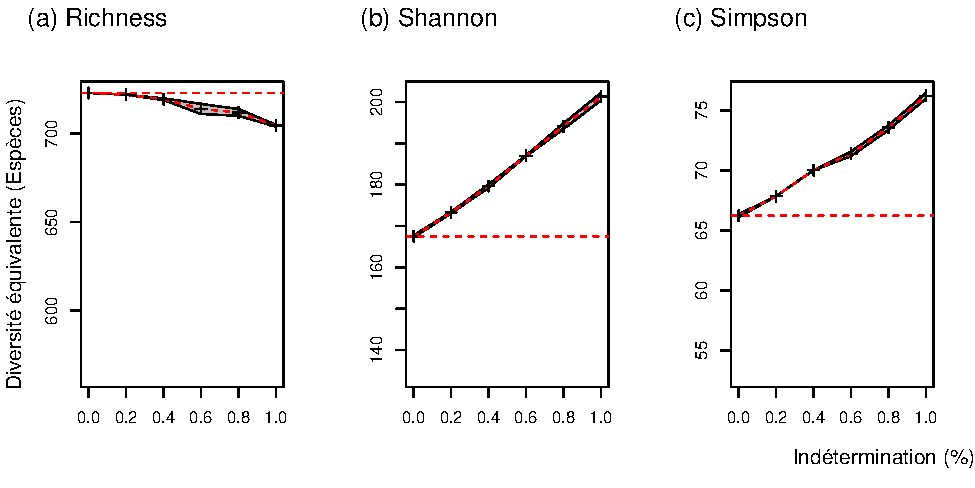
\includegraphics[width=1\linewidth]{Manuscript_files/figure-latex/FigTreesSp-1} 

}

\caption{Biais de l'estimateur pour les diversité de \textbf{(a)} Richesse, \textbf{(b)} Shannon et \textbf{(c)} Simpson selon un gradient d'indétermination taxonomique. L'envelope grise représente l'intervalle de confiance à 95\% de l'estimateur.}\label{fig:FigTreesSp}
\end{figure*}

Les estimateurs de richesse et d'équitabilité (diversité de Shannon et
Simpson) sont d'autant plus biaisés que le degré d'indétermination est
élevé. Tandis que la richesse est sous-estimée, l'équitabilité est
sur-estimée: l'estimateur tend donc à homogénéiser les distributions
d'abondance. Un nom vernaculaire a plus de chances d'être associé à une
espèce abondante (plus fréquente) qu'à une espèce rare et donc la queue
de distribution en espèces rares n'est pas correctement reproduite. Ce
biais de l'estimateur semble difficile à formaliser car il dépend de la
relation entre rareté et probabilité d'indétermination des espèces, ce
qui rend pour le moment difficile toute correction formelle.

Dans la suite de ce travail nous avons choisi de pallier ce biais de
l'estimateur en nous rapportant au niveau taxonomique supérieur et en
étudiant la diversité au niveau du genre botanique. Dans le cas d'une
mesure rapportée au genre, l'estimateur de la richesse reste peu biaisé
jusqu'à un seuil d'indétermination de 80\% au delà duquel la richesse
est trop sous-estimée. L'équitabilité est surestimée, d'autant plus que
le degré d'indétermnation est élevé (diversités de Shannon et de
Simpson), mais le biais ne dépasse pas 10\% de la diversité réelle
\ref{fig:FigTreesGenus}.

Dans le cas de Paracou, la détermination des parcelles est variable au
cours du temps et entre les parcelles. Au moment de travail, dans les
parcelles contrôle et du traitement 3 moins de 5\% des arbres n'ont pas
d'identification botanique, tandis que les parcelles du traitement 1 ou
2 restent mal déterminées (30\% d'indétermination pour certaines
parcelles). Les trajectoires de diversité seront donc étudiées en termes
de différence à l'état initial de chaque parcelle. Pour l'état initial
nous prendrons comme référence les inventaires 5 ans après exploitation,
date à partir de laquelle l'incertitude des inventaires reste stable.

\begin{figure*}

{\centering 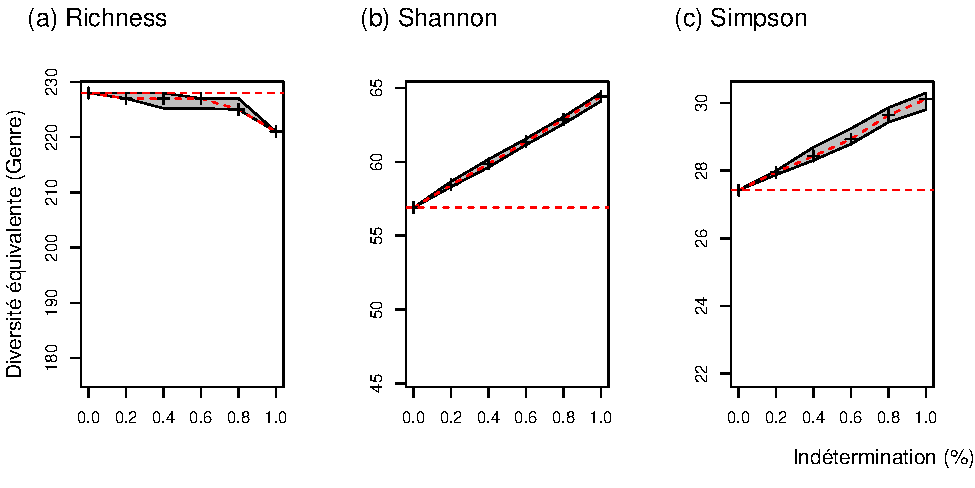
\includegraphics[width=0.6\linewidth]{Manuscript_files/figure-latex/FigTreesGenus-1} 

}

\caption{Biais de l'estimateur pour les diversité en genre botanique de \textbf{(a)} Richesse, \textbf{(b)} Shannon et \textbf{(c)} Simpson selon un gradient d'indétermination taxonomique. L'envelope grise représente l'intervalle de confiance à 95\% de l'estimateur.}\label{fig:FigTreesGenus}
\end{figure*}

\section{Application de l'estimateur au cas des inventaires
pré-exploitation}\label{application-de-lestimateur-au-cas-des-inventaires-pre-exploitation}

Comprendre et anticiper le devenir des forêts tropicales dans le
contexte actuel requiert un suivi temporel des communautés et des
mesures de diversité précis. Le coût des inventaires forestiers conduit
cependant la majorités à être réalisés en noms vernaculaires, malgré que
ceux-ci impliquent d'importances incertitudes taxonomiques. Plusieurs
méthodes ont été proposées pour pallier ces incertitudes mais aucune
n'est encore adaptée à des suivi de diversité fonctionnelle ou à petite
échelle spatiale. Nous proposons ici un estimateur de diversité
adaptable à chaque inventaire particulier et intégrant les incertitudes
botaniques inhérentes aux inventaires forestiers. Nous avons calibré
l'estimateur de diversité à partir d'un large inventaire en forêt
Néotropicale et la simulation de gradients d'incertitude taxonomique et
d'effort d'échantillonnage ont permis de déterminé un protocole
d'inventaire idéal optimisant le coût des inventaires et la précision de
l'estimateur. Notre analyse a d'une part souligné la nécessité d'avoir
recours à des inventaires réels et à une expertise botanique de terrain
par assurer la fiabilité de mesures de diversité. D'autre part nous
avons pu identifié un protocole idéal assurant une estimation de la
diversité avec un intervalle de confiance de 10\%, basé sur l'inventaire
de 3 000 arbres au minimum et sur une effort d'identification
taxonomique de 80\% des espèces.

\newpage

\section*{Inescapable Taxonomists: Workable Biodiversity Management
Based on a Minimum Field
Work}\label{inescapable-taxonomists-workable-biodiversity-management-based-on-a-minimum-field-work}
\addcontentsline{toc}{section}{Inescapable Taxonomists: Workable
Biodiversity Management Based on a Minimum Field Work}

\subsection{Abstract}\label{abstract}

Assess the fate of Neotropical forests requires to accurately measures
forest diversity and reliably monitor forest communities. The costs of
botanical inventories and the taxonomic complexity of Neotropical
forests make forest inventories in vernacular names the most efficient
approach today, although these hold high botanical uncertainty and limit
the accuracy of diversity measures. Several methods were proposed to
compensate these botanical uncertainties but none reliably assessed
functional and fine-scale diversity surveys. We developed a polyvalent
diversity estimator workable in numerous specific cases based on the
propagation of botanical uncertainties. The estimator was calibrated
with a large neotropical inventory and the simulations of uncertainty
and sampling effort gradients allowed to determined an ideal inventory
protocol optimizing the costs and the accuracy of forest inventories.\\
Our study first advocated of necessity of real inventories and the
inescapable recourse to taxonomists to ensure reliable diversity
estimations. An ideal inventory protocol based on a sampling effort of 3
000 trees and on an identification effort of 80\% of the species was
identified and ensured diversity estimations with a 10\% error.

\subsection{Introduction}\label{introduction}

The variety of tree species, their assemblages in space and their
dynamics in time are determinant of forests productivity and functioning
\autocite{Cardinale2012}. Preserve tree diversity is crucial to maintain
forests functioning and services, specifically in hyper-diverse tropical
forests where the biodiversity is as threatened as it is valuable and
unexplored \autocite{Barlow2018}. Handling the conservation and
management of tree diversity requires setting sensible protection areas
and sustainable forest management calibrated according to diversity
patterns in space and time and their determinants
\autocites{Margules2000}{Purvis2000}{Gibson2011a}{FAO2014}{Sist2015}.

Correctly measure, map and manage forests biodiversity require accurate
and large forest monitoring. The precision of forest inventories,
though, is often limited by their significant cost in terms of time,
money, and logistic \autocites{Feeley2011}{Baraloto2013}. Sampling
methods were optimized to minimize these costs and maximize inventory
accuracy.Some approaches would restrict inventories to some DBH or
height classes, to specific taxa, or would opt for inventories at family
or genus level. These methods efficiently translated biodiversity
patterns at regional scales and along wide ecological gradients
\autocites{Steege2000}{Higgins2004}{Rejou-Mechain2011}{Pos2014}.
However, these methods were either limited to small areas (under 1ha),
sometimes remained biased or holding significant uncertainty, and
usually proved limited to detect subtle diversity aspects and to
desentangle richness from equitability parameters
\autocites{Phillips2003a}{Baraloto2013}[
]{Guitet2014b}{Vellend2008}{Prance1994}. Another approach proposed to
use inventories in vernacular names instead of botanical species.
Vernacular names indeed are easier to attribute, more common and usually
do not require vouchers collection or posterior botanical
identification. The reliability of vernacular names may be high at genus
level, but this proved highly variable across tropical regions: while
this reliability was estimated around 60-70\% in French Guiana
\autocites{Hawes2012}{Guitet2014b} to ranges from 32\% to 67\% in
Central Africa \autocite{Rejou-Mechain2011}. The multiple and variable
associations between botanical and vernacular names then entail
significant botanical uncertainties that should not be ignored
\autocite{Oldeman1968}. Besides, rough vernacular inventories would not
allow functional and phylogenetic approaches, that require
identification at the botanical species to comply with phylogenetic and
functional database. However the approach through vernacular names
deserves further attention. First, it gives the opportunity to analyze
pre-logging inventories conducted in large areas by logging companies.
Second, as exhaustive inventories, they allow some post-process based on
vernacular/botanical names association and allow the building of
reliable diversity estimators
\autocites{TerSteege2006}{Feldpausch2006}{Rejou-Mechain2008}{Rejou-Mechain2011}.
Following this idea \textcite{Guitet2014b} proposed a framework
propagating vernacular names taxonomic uncertainties in diversity
measures. The propagation framework was based on Monte-Carlo processes
estimating forest diversity from the vernacular-botanical name
association. These association combined prior information from both
general taxa-abundance correspondence table \autocite{Molino2009} and
reference field inventories. The framework successfully rendered the
ranking of plots diversity, but remained restricted to large
environmental gradient and for highly different communities
\autocites{Guitet2014b}{Guitet2013}. In this study we offer to refine
this framework and adapt it to diversity estimation at smaller spatial
scales. The following diversity estimator is based on the specific case
of the studied community and the inventory protocol. The diversity
estimator besides suits all inventories whatever the ratio of botanical
determination, \emph{i.e.} ratio of vernacular compared to botanical
names. It besides suits experimental specific as well as pre-logging
inventories where only the commercial or most recognizable species are
identified at species level.

Such diversity estimator allows maximizing the accuracy of diversity
measures while minimizing the sampling effort, \emph{i.e.} the size of
inventoried communities and the number of accurately identified species.
In this perspective we thought to calibrate an ideal inventory protocol
optimized in terms of sampling effort and determination degree. From a
real inventory, with complete vernacular and botanical identifications,
we simulated ranges of sampling efforts and identification degrees along
which we examined the bias and variability of the diversity estimator.

In this study we \emph{(i)} redesigned a diversity estimator based on a
Bayesian framework accounting for both general taxa-association tables
and specific field inventories, and \emph{(ii)} applied the estimator to
a real Neotropical forest inventory to determine the sampling effort and
determination degree of an ideal inventory protocol.

\subsection{Methods}\label{methods}

\subsubsection{Study community}\label{study-community}

We based our analyses on the inventory of a Neotropical rainforest, from
the Paracou Research Station in French Guiana (5°18'N and 52°53'W). The
experimental site stands in a lowland tropical rainforest with a flora
dominated by \emph{Fabaceae}, \emph{Chrysobalanaceae},
\emph{Lecythidaceae} and \emph{Sapotaceae} families. Mean mean annual
temperature is 26°C. and the mean annual precipitations average
\(2980 mm.y^-1\) (30-y period) with a 3-months dry season
(\(< 100 mm.months-1\)) from mid-August to mid-November and a one-month
dry season in March \autocite{Wagner2011}. Elevation ranges between 5
and 50 m and soils correspond to thin acrisols over a layer of
transformed saprolite with low permeability, generating lateral drainage
during heavy rains \autocite{IUSSWorkingGroupWRB2015}. We used the 2015
inventory of six permanent plots of undisturbed forest (6.25ha each,
37.5ha inventoried in total). During inventories trees are identified
first with a vernacular name assigned by the forest worker team, and
afterward with a scientific name assigned by botanists during regular
botanical campaigns. The community inventoried ancompasses 22 904 trees
belonging to 375 species and 63 families, identified by 290 different
vernacular names. The initial taxonomic uncertainty was 3\% of the
community, \emph{i.e.} the proportion of trees not identified with a
botanical name.

\subsubsection{Diversity measures}\label{diversity-measures}

Among the large panel of diversity indices we examined here the family
of q-generalized (Tsallis) entropy, widely adopted to assess all aspects
of taxonomic, functional and phylogenetic diversities. The Tsallis
diversity indices derive from a general formula, modulated by an order q
emphasizing species frequency \eqref{eq:TsallisEntropy}.

\begin{equation}
^qD = \sum_{i=1}^{N}{\left( p_i^q \right)^{\frac{1}{1-q}} }
\label{eq:TsallisEntropy}
\end{equation}

In the diversity formula, species relative abundance \(p_i\) in a
community of \(N\) species is raised at the power \(q\) that is the
order of the diversity. The higher the order \(q\), the higher the
emphasis on common vs.~rare species, so browsing a range of order \(q\)
corresponds assess a gradient balance between richness and evenness. The
formula retrieves species richness for \(q = 0\) , Shannon diversity for
\(q = 1\) where richness and evenness are equally accounted for and
Simpson diversity, that can be undestood as the diversity of common
species, for \(q = 2\). The Tsallis diversity indices would eventually
be converted into equivalent number of species in our framework. The
conversion in equivalent number of species, through Hill transformation,
allows understandable analysis and comparisons among communities
\autocites{Hill1973}{Keylock2005}{Jost2006}.

\subsubsection{Diversity estimator}\label{diversity-estimator}

The estimation framework is based on the diversity distribution measured
on theoretical, fully determined communities. Theoretical inventories
are simulated 1 000 times from the real incomplete inventory, through
the replacement by a Monte-Carlo scheme of vernacular names by botanical
ones.

The vernacular-botanical replacement are based on the association
probability between each vernacular names and the botanical names
inventoried. For each vernacular name the association model follows a
multinomial distribution
\(M([s_1, s_2, …, s_N] ,[\alpha_1, \alpha_2,…, \alpha_N])\), with
\([\alpha_i]\) the association probability of botanical name \(s_i\)
with the vernacular name.

The association probability vectors \([\alpha_v]\) were determined with
a Bayesian framework based on the combination of botanical expertise and
observed associations. First, the estimation of \([\alpha_v]\) accounted
for prior information from experts' knowledge in the form of a general
taxa-association table listing all botanical names likely corresponding
to the vernacular name \(v\). From this general table, the probability
\(\lambda_i={}^1/m_v\) was attributed to each of the \(m_v\) botanical
names with a confirmed association with \(v\). When no association was
established the probability \(\lambda_i={}^\epsilon\big/_{N-m_v}\) was
attributed to the botanical name, with \(\epsilon\) standing for a
background noise set to 0.01 here. Second, the estimation of
\([\alpha_v]\) accounted for observed inventories giving real
association frequencies \(\phi_i\) between \(v\) and the \(m_v'\)
botanical names with observed association. Similarly, the association
probability \(\lambda_i={}^\epsilon\big/_{N-m_v'}\) was attributed to
botanical names with no observed association. The final \([\alpha_v]\)
distribution was modeled by a Multinomial-Dirichlet scheme combining the
two vectors \([\lambda^v]\) and \([\phi^v]\) \autocite{McCarthy2007}.

To test the relevance of the general table and observed inventories
information, we tested a range of weighting \(w\). Assuming a
distribution of \([\phi^v]\) conditionally to \([\alpha^v]\) the
weighting returned the formula \eqref{eq:weighting}.

\begin{equation}
[\alpha_i^v]: 
\Big[\alpha_i^v | _{(1-w)\lambda_i^v ,w.\phi_i^v}\Big] =Dirichlet\Big((1-w)\phi_i^v+w.\lambda_i^v\Big)
\label{eq:weighting}
\end{equation}

When \(w=0\) only observed inventories were considered, when \(w=0.5\)
both information were equally accounted for and when \(w=1\) only the
general taxa-association table was considered.

\subsubsection{Simulation of determination and sampling effort
gradients}\label{simulation-of-determination-and-sampling-effort-gradients}

The estimator was calibrated in comparing several methods for the
vernacular/botanical association probability (corresponding to different
values of \(w\), the balance between general table and observed
inventories). The performance of the estimator was examined regarding
its bias, \emph{i.e.} the difference between the estimation and the real
diversity, and its variability, \emph{i.e.} 95\% confidence interval
\autocite{Baltanas2009}. For each computation method the performance of
the estimator was examined along a determination gradient (corresponding
to an increasing number of species only identified in vernacular name).
As rare species had more chance to be undetermined (Kendall test,
\(\tau = -0.46, p < 10^-16\)), the trial of ignored determination
followed botanical names abundance (\(p_{undetermined}=f_i^{-0.1}\),
with \(f_i\) botanical name frequency).

Different inventory specific cases were then tested in examining the
bias and variability of the estimator along a sampling effort gradient
(corresponding to an increasing number of trees, from 500 to 22 000
trees, used to compute the vernacular/botanical association
probability). Along the sampling effort gradient the estimations were
performed on the fully undetermined inventory, \emph{i.e.} without any
botanical identification.

\subsection{Results}\label{results}

\subsubsection{The reponse to determination effort, and the design of an
ideal
framework}\label{the-reponse-to-determination-effort-and-the-design-of-an-ideal-framework}

Along the indetermination gradient, when considering both general
taxa-association table and observed inventory the diversity was
increasingly overestimated (Fig. \ref{fig:UncertGrad}). This
overestimation increased with the order of diversity q, while it was not
significant for the richness (\(q=0\)), the overestimation reached 45\%
of the real diversity for Shannon diversity (\(q = 1\)) and it reached
57\% of the real diversity for the Simpson diversity (\(q = 2\)).

When only considering the general taxa-association table the richness
(\(q=0\)) was underestimated (reaching a 50\% underestimation), while
both Shannon and Simpson diversities were overestimated (respectively
reaching underestimations of 67\% and 125\%).

When only considering the observed inventory the estimator remained
slightly biased but it did not exceed 15\% of the real diversity for any
order of diversity.

A bootstrap of the 100 simulations for each specific case and diversity
order showed a stabilization of variances after 60 simulations.

\begin{figure*}

{\centering 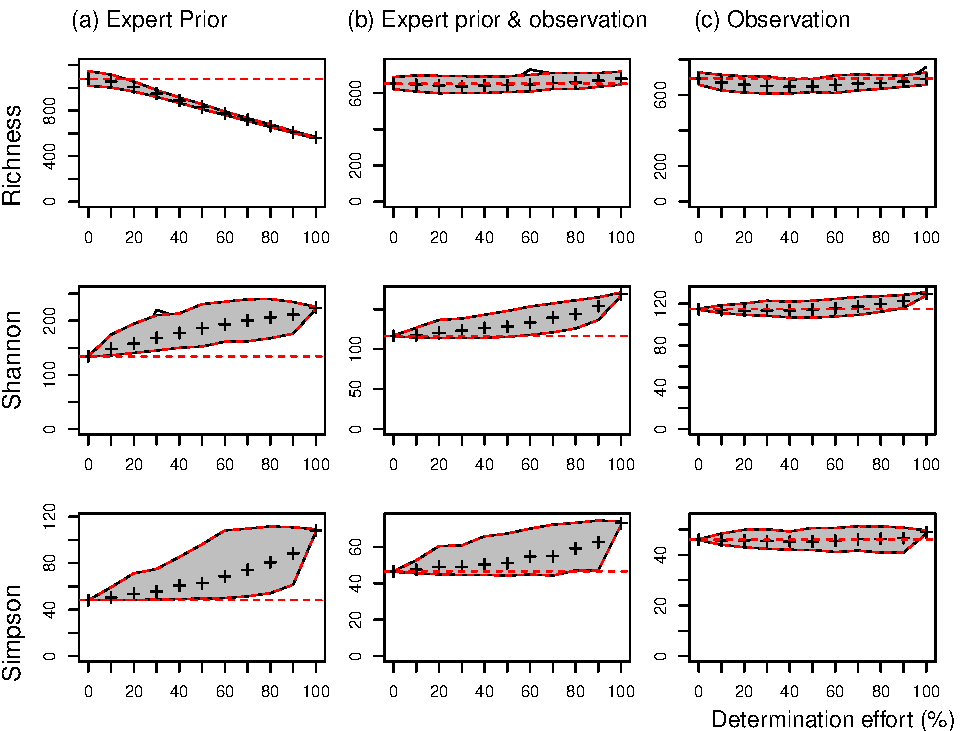
\includegraphics[width=1\linewidth]{Manuscript_files/figure-latex/UncertGrad-1} 

}

\caption{Richness, Shannon and Simpson estimator bias and 95\%confidence interval along an uncertainty gradient with the association frequencies computed from (a) only expert prior, (b) both expert and observation prior and (c) only observation prior.}\label{fig:UncertGrad}
\end{figure*}

\subsubsection{Calibrating the sampling
effort}\label{calibrating-the-sampling-effort}

Along the sampling effort gradient from 500 to 22 000 trees, the
richness estimator remained negatively biased but the confidence
interval did not exceed 7\%. The Shannon and Simpson were less biased,
for 3 000 trees inventoried the Shannon diversity bias fell to 15\%
while the bias of Simpson estimator fell to 6\% (Fig.
\ref{fig:SEgradient}).

\begin{figure*}

{\centering 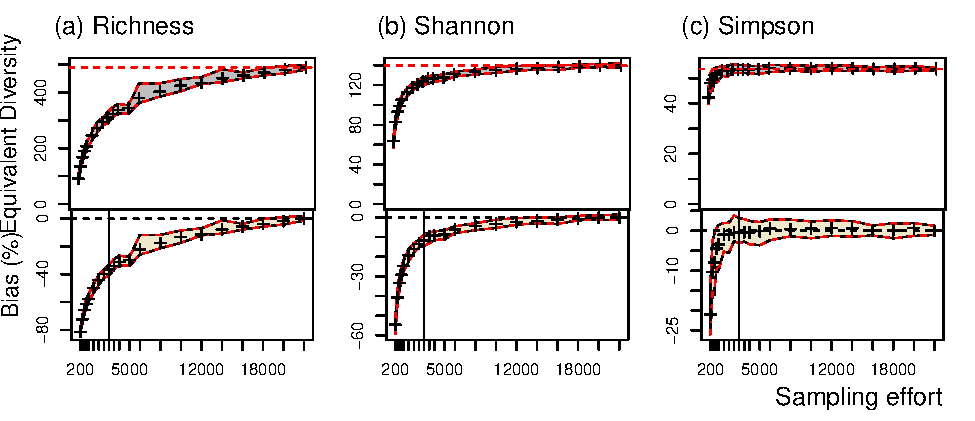
\includegraphics[width=1\linewidth]{Manuscript_files/figure-latex/SEgradient-1} 

}

\caption{Richness, Shannon and Simpson estimation (upper panels) and bias compared to real diversity (lower panels) along a sampling effort gradient. Shaded areas are the 95\% confidence intervals, vertical plain line stands for the points at 3 000 trees.}\label{fig:SEgradient}
\end{figure*}

The precision and bias of the estimator were eventually tested for the
recomended sampling effort of 3 000 trees. In this case the Shannon and
Simpson biases remained lower than 10\% and the Richness bias was below
10\% until 20\% of undetermined species.

\begin{figure*}

{\centering 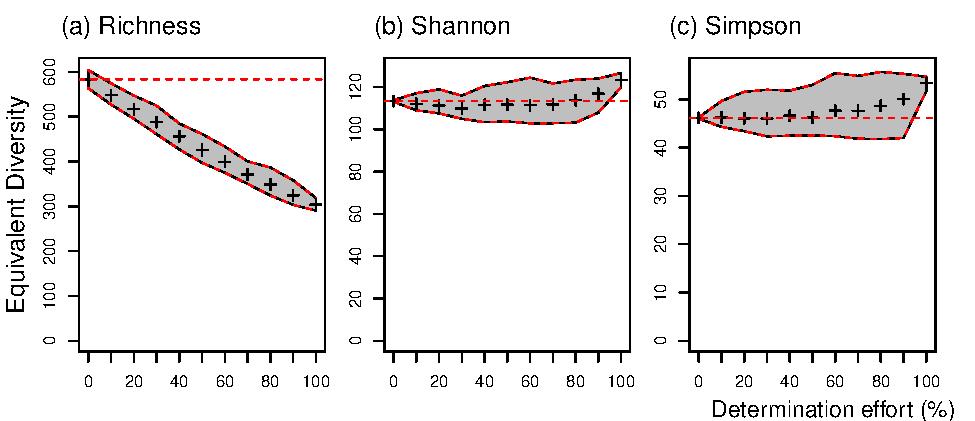
\includegraphics[width=1\linewidth]{Manuscript_files/figure-latex/UncertGradLim-1} 

}

\caption{Richness, Shannon and Simpson estimators along a taxonomic uncertainty gradient based on field inventories of 3 000 trees,  with shaded areas the 95\% confidence interval.}\label{fig:UncertGradLim}
\end{figure*}

\subsection{Discussion}\label{discussion}

\subsubsection{Inescapable taxonomists}\label{inescapable-taxonomists}

The method developed in the line of \textcite{Guitet2014b} to propagate
the taxonomic uncertainty of vernacular names in diversity mesures
provided a reliable estimator for diversity indices, workable for all
diversity order and adaptable for functoinal diversity. The use the
general taxonomic-association table proved to systematically
overestimate the diversity. In these tables the vernacular/botanical
association probabilities were independent of botanical name abundances,
so rare vernacular names were indifferently replaced by rare or abundant
botanical names. As a result, the abundance of rare species were
inflated at the expense abundant ones, which overestimated the
equitability. Contrastingly the use of observed inventories that account
for the abundance of botanical names proved more reliable. The rescourse
to taxonomists and pre-inventories proved unavoidable to correctly
estimate and therefore manage forest biodiversity.

\subsubsection{Calibration of an optimized inventory
protocol}\label{calibration-of-an-optimized-inventory-protocol}

The performance of the estimator, regarding its bias and variability,
along the determination and sampling efforts gradients highlighted the
difficulty to assess communities richness. Whatever the inventory
protocol the richness indeed remained significantly biased, as already
suggested in previous analysis comparing several inventory methods
\autocite{Higgins2004}.

Conversely, the Shannon and Simpson diversity estimations proved less
biased, thus allowing the estimator to detect small variation of
community equitability. This would be a key to value existing
inventories and ease future protocols as subtle time and spatial
diversity variations often invlove changes in community abundance
distribution rather than richness
\autocites{Baraloto2012a}{Berry2008a}{Cannon1998}{Plumptre1996}.

An optimized protocol maximizing the estimator performance on the one
hand and minimizing the determination and sampling efforts on the other
hand corresponding to the pre-inventory of at least 3 000 trees and the
determination of 80\% of the botanical species.

\subsection{Conclusion}\label{conclusion}

The diversity estimator developed in this paper (i) proved relevant to
measure tropical forest diversity at small time and spatial scale, (ii)
allowed to integrate the specificities of local forests and working
team, and (iii) was adaptable for both taxonomic and functional
diversity at all order. Examining the estimator performance highlighted
the inescapable rescourse to taxonomists and to minimum real
inventories: an initial inventory of 3 000 trees with 80\% of the
species identified allowed an estimation accurate at 10\% of Shannon and
Simpson diversities. The diversity estimator allows integrating and is
thus adaptable to all specific case.

\newpage

\section{Script R, estimateur de
diversité}\label{script-r-estimateur-de-diversite}

L'estimateur de diversité correspond à la routine présentée ci-dessous.
L'estimateur utilise les fonctions du package entropart
\autocite{Entropart2015}. La donnée d'entrée est un inventaire sous
forme de tableau recensant les individus inventoriés en ligne et les
informations botaniques correspodantes en colonne (nom vernaculaire,
famille, genre et espèce).

Le script retourne la moyenne et l'intervalle de confiance à 95\% du
profil de diversité d'un inventaire. L'inventaire est une matrice Plot
(individu * données botaniques), les données manquantes sont notées
``Indet.''

\begin{verbatim}
##      Vernacular        Family     Genus    Species
## 626  busi mango    Clusiaceae  Tovomita     Indet.
## 3   maho cochon     Malvaceae Sterculia   pruriens
## 8    maho rouge Lecythidaceae  Lecythis persistens
## 4          wapa      Fabaceae    Eperua    falcata
## 815        weko      Fabaceae      Inga     Indet.
\end{verbatim}

La première étape donne une matrice alpha d'association
vernaculaire/botanique qui liste les fréquences d'association observées
dans l'inventaire de référence.

\begin{Shaded}
\begin{Highlighting}[]
\NormalTok{alpha_construct <-}\StringTok{ }\ControlFlowTok{function}\NormalTok{(Plot) \{}
\NormalTok{    mat_eff <-}\StringTok{ }\KeywordTok{as.data.frame.matrix}\NormalTok{(}\KeywordTok{with}\NormalTok{(Plot, }\KeywordTok{xtabs}\NormalTok{(}\OperatorTok{~}\NormalTok{name }\OperatorTok{+}\StringTok{ }\NormalTok{Vernacular)))}
    
\NormalTok{    alpha <-}\StringTok{ }\KeywordTok{apply}\NormalTok{(mat_eff, }\DecValTok{2}\NormalTok{, }\ControlFlowTok{function}\NormalTok{(v) \{}
\NormalTok{        v}\OperatorTok{/}\KeywordTok{sum}\NormalTok{(v)}
\NormalTok{    \})}
    
    \KeywordTok{return}\NormalTok{(alpha)}
\NormalTok{\}}
\end{Highlighting}
\end{Shaded}

A partir d'un vecteur d'association, un processus Dirichlet/Multinomial
permet de tirer au hasard un nom botanique

\begin{Shaded}
\begin{Highlighting}[]
\NormalTok{Dirichlet_draw <-}\StringTok{ }\ControlFlowTok{function}\NormalTok{(V) \{}
\NormalTok{    Vdir <-}\StringTok{ }\NormalTok{gtools}\OperatorTok{::}\KeywordTok{rdirichlet}\NormalTok{(}\DecValTok{1}\NormalTok{, V)}
    \KeywordTok{names}\NormalTok{(Vdir) <-}\StringTok{ }\KeywordTok{names}\NormalTok{(V)}
\NormalTok{    res <-}\StringTok{ }\KeywordTok{rmultinom}\NormalTok{(}\DecValTok{1}\NormalTok{, }\DecValTok{1}\NormalTok{, Vdir)}
\NormalTok{    res <-}\StringTok{ }\KeywordTok{rownames}\NormalTok{(res)[}\KeywordTok{which}\NormalTok{(res }\OperatorTok{>}\StringTok{ }\DecValTok{0}\NormalTok{)]}
    \KeywordTok{return}\NormalTok{(res)}
\NormalTok{\}}
\end{Highlighting}
\end{Shaded}

Pour tenir compte de toute les informations phylogénétiques disponibles,
on liste les associations possibles nom vernaculaire / Famille / genre /
espèce

\begin{Shaded}
\begin{Highlighting}[]
\NormalTok{Correspondences <-}\StringTok{ }\ControlFlowTok{function}\NormalTok{(Plot) \{}
\NormalTok{    bota <-}\StringTok{ }\NormalTok{Plot[}\KeywordTok{order}\NormalTok{(Plot[, }\StringTok{"Family"}\NormalTok{], Plot[, }\StringTok{"Genus"}\NormalTok{], Plot[, }\StringTok{"Species"}\NormalTok{]), }
\NormalTok{        ]}
\NormalTok{    bota <-}\StringTok{ }\NormalTok{bota[}\KeywordTok{which}\NormalTok{(}\OperatorTok{!}\KeywordTok{duplicated}\NormalTok{(bota)), ]}
    \KeywordTok{return}\NormalTok{(bota)}
\NormalTok{\}}
\end{Highlighting}
\end{Shaded}

On peut alors attribuer un nom botanique à tout nom vernaculaire:

\begin{Shaded}
\begin{Highlighting}[]
\NormalTok{tirage <-}\StringTok{ }\ControlFlowTok{function}\NormalTok{(alpha, bota, name, }\DataTypeTok{eps =} \FloatTok{0.05}\NormalTok{) \{}
    
    \ControlFlowTok{if}\NormalTok{ (name[}\StringTok{"Vernacular"}\NormalTok{] }\OperatorTok{==}\StringTok{ "-"}\NormalTok{) \{}
\NormalTok{        trial <-}\StringTok{ }\KeywordTok{sample}\NormalTok{(}\KeywordTok{rownames}\NormalTok{(alpha), }\DecValTok{1}\NormalTok{)}
        \ControlFlowTok{while}\NormalTok{ (}\KeywordTok{grepl}\NormalTok{(}\StringTok{"Indet."}\NormalTok{, trial)) \{}
\NormalTok{            trial <-}\StringTok{ }\KeywordTok{sample}\NormalTok{(}\KeywordTok{rownames}\NormalTok{(alpha), }\DecValTok{1}\NormalTok{)}
\NormalTok{        \}}
\NormalTok{    \}}
    
\NormalTok{    alpha_adjust <-}\StringTok{ }\NormalTok{alpha[, name[}\StringTok{"Vernacular"}\NormalTok{]]}
    
    \ControlFlowTok{if}\NormalTok{ (name[}\StringTok{"Vernacular"}\NormalTok{] }\OperatorTok{!=}\StringTok{ "-"} \OperatorTok{&}\StringTok{ }\NormalTok{name[}\StringTok{"Genus"}\NormalTok{] }\OperatorTok{!=}\StringTok{ "Indet."}\NormalTok{) \{}
        
\NormalTok{        mismatch <-}\StringTok{ }\NormalTok{bota[}\KeywordTok{intersect}\NormalTok{(}\KeywordTok{which}\NormalTok{(bota[, }\StringTok{"Vernacular"}\NormalTok{] }\OperatorTok{==}\StringTok{ }\NormalTok{name[}\StringTok{"Vernacular"}\NormalTok{]), }
            \KeywordTok{which}\NormalTok{(}\OperatorTok{!}\NormalTok{bota[, }\StringTok{"Genus"}\NormalTok{] }\OperatorTok\StringTok{ }\NormalTok{name[}\StringTok{"Genus"}\NormalTok{])), }\StringTok{"name"}\NormalTok{]}
        
\NormalTok{        alpha_adjust[}\KeywordTok{as.character}\NormalTok{(mismatch)] <-}\StringTok{ }\DecValTok{0}
\NormalTok{        match <-}\StringTok{ }\KeywordTok{names}\NormalTok{(alpha_adjust[}\KeywordTok{which}\NormalTok{(alpha_adjust }\OperatorTok{!=}\StringTok{ }\DecValTok{0}\NormalTok{)])}
        
\NormalTok{        alpha_adjust[}\KeywordTok{which}\NormalTok{(alpha_adjust }\OperatorTok{==}\StringTok{ }\DecValTok{0}\NormalTok{)] <-}\StringTok{ }\NormalTok{eps}\OperatorTok{/}\KeywordTok{length}\NormalTok{(}\KeywordTok{which}\NormalTok{(alpha_adjust }\OperatorTok{==}\StringTok{ }
\StringTok{            }\DecValTok{0}\NormalTok{))}
        
\NormalTok{        trial <-}\StringTok{ }\KeywordTok{Dirichlet_draw}\NormalTok{(alpha_adjust)}
        
        \ControlFlowTok{if}\NormalTok{ (}\KeywordTok{any}\NormalTok{(}\KeywordTok{grep}\NormalTok{(}\StringTok{"Indet."}\NormalTok{, match, }\DataTypeTok{invert =}\NormalTok{ T) }\OperatorTok{!=}\StringTok{ }\DecValTok{0}\NormalTok{)) \{}
            \ControlFlowTok{while}\NormalTok{ (}\KeywordTok{grepl}\NormalTok{(}\StringTok{"Indet."}\NormalTok{, trial)) \{}
\NormalTok{                trial <-}\StringTok{ }\KeywordTok{Dirichlet_draw}\NormalTok{(alpha_adjust)}
\NormalTok{            \}}
\NormalTok{        \}}
\NormalTok{    \}}
    
    \CommentTok{# Seuls les noms botaniques correspondant aux informations botaniques sont}
    \CommentTok{# gardés dans le tirage}
    
    \ControlFlowTok{if}\NormalTok{ (name[}\StringTok{"Vernacular"}\NormalTok{] }\OperatorTok{!=}\StringTok{ "-"} \OperatorTok{&}\StringTok{ }\NormalTok{name[}\StringTok{"Genus"}\NormalTok{] }\OperatorTok{==}\StringTok{ "Indet."} \OperatorTok{&}\StringTok{ }\NormalTok{name[}\StringTok{"Family"}\NormalTok{] }\OperatorTok{!=}\StringTok{ }
\StringTok{        "Indet."}\NormalTok{) \{}
        
\NormalTok{        mismatch <-}\StringTok{ }\NormalTok{bota[}\KeywordTok{intersect}\NormalTok{(}\KeywordTok{which}\NormalTok{(bota[, }\StringTok{"Vernacular"}\NormalTok{] }\OperatorTok{==}\StringTok{ }\NormalTok{name[}\StringTok{"Vernacular"}\NormalTok{]), }
            \KeywordTok{which}\NormalTok{(}\OperatorTok{!}\NormalTok{bota[, }\StringTok{"Family"}\NormalTok{] }\OperatorTok\StringTok{ }\NormalTok{name[}\StringTok{"Family"}\NormalTok{])), }\StringTok{"name"}\NormalTok{]}
        
\NormalTok{        alpha_adjust[}\KeywordTok{as.character}\NormalTok{(mismatch)] <-}\StringTok{ }\DecValTok{0}
\NormalTok{        match <-}\StringTok{ }\KeywordTok{names}\NormalTok{(alpha_adjust[}\KeywordTok{which}\NormalTok{(alpha_adjust }\OperatorTok{!=}\StringTok{ }\DecValTok{0}\NormalTok{)])}
        
\NormalTok{        alpha_adjust[}\KeywordTok{which}\NormalTok{(alpha_adjust }\OperatorTok{==}\StringTok{ }\DecValTok{0}\NormalTok{)] <-}\StringTok{ }\NormalTok{eps}\OperatorTok{/}\KeywordTok{length}\NormalTok{(}\KeywordTok{which}\NormalTok{(alpha_adjust }\OperatorTok{==}\StringTok{ }
\StringTok{            }\DecValTok{0}\NormalTok{))}
        
\NormalTok{        trial <-}\StringTok{ }\KeywordTok{Dirichlet_draw}\NormalTok{(alpha_adjust)}
        \ControlFlowTok{if}\NormalTok{ (}\KeywordTok{any}\NormalTok{(}\KeywordTok{grep}\NormalTok{(}\StringTok{"Indet."}\NormalTok{, match, }\DataTypeTok{invert =}\NormalTok{ T)) }\OperatorTok{!=}\StringTok{ }\DecValTok{0}\NormalTok{) \{}
            \ControlFlowTok{while}\NormalTok{ (}\KeywordTok{grepl}\NormalTok{(}\StringTok{"Indet."}\NormalTok{, trial)) \{}
\NormalTok{                trial <-}\StringTok{ }\KeywordTok{Dirichlet_draw}\NormalTok{(alpha_adjust)}
\NormalTok{            \}}
\NormalTok{        \}}
\NormalTok{    \}}
    \ControlFlowTok{if}\NormalTok{ (name[}\StringTok{"Vernacular"}\NormalTok{] }\OperatorTok{!=}\StringTok{ "-"} \OperatorTok{&}\StringTok{ }\NormalTok{name[}\StringTok{"Genus"}\NormalTok{] }\OperatorTok{==}\StringTok{ "Indet."} \OperatorTok{&}\StringTok{ }\NormalTok{name[}\StringTok{"Family"}\NormalTok{] }\OperatorTok{==}\StringTok{ }
\StringTok{        "Indet."}\NormalTok{) \{}
        
\NormalTok{        alpha_adjust[}\KeywordTok{which}\NormalTok{(alpha_adjust }\OperatorTok{==}\StringTok{ }\DecValTok{0}\NormalTok{)] <-}\StringTok{ }\NormalTok{eps}\OperatorTok{/}\KeywordTok{length}\NormalTok{(}\KeywordTok{which}\NormalTok{(alpha_adjust }\OperatorTok{==}\StringTok{ }
\StringTok{            }\DecValTok{0}\NormalTok{))}
        
\NormalTok{        trial <-}\StringTok{ }\KeywordTok{Dirichlet_draw}\NormalTok{(alpha_adjust)}
        \ControlFlowTok{while}\NormalTok{ (}\KeywordTok{grepl}\NormalTok{(}\StringTok{"Indet."}\NormalTok{, trial)) \{}
\NormalTok{            trial <-}\StringTok{ }\KeywordTok{Dirichlet_draw}\NormalTok{(alpha_adjust)}
\NormalTok{        \}}
\NormalTok{    \}}
    \KeywordTok{return}\NormalTok{(trial)}
\NormalTok{\}}
\end{Highlighting}
\end{Shaded}

On peut alors générer un inventaire théorique complet à partir de
l'inventaire réel

\begin{Shaded}
\begin{Highlighting}[]
\NormalTok{Replacement <-}\StringTok{ }\ControlFlowTok{function}\NormalTok{(Plot, Alpha, Bota) \{}
\NormalTok{    Determ <-}\StringTok{ }\NormalTok{Plot[}\KeywordTok{which}\NormalTok{(}\OperatorTok{!}\NormalTok{Plot[}\StringTok{"Species"}\NormalTok{] }\OperatorTok{==}\StringTok{ "Indet."}\NormalTok{), ]}
\NormalTok{    Indet <-}\StringTok{ }\NormalTok{Plot[}\KeywordTok{which}\NormalTok{(Plot[}\StringTok{"Species"}\NormalTok{] }\OperatorTok{==}\StringTok{ "Indet."}\NormalTok{), ]}
    
\NormalTok{    Vern <-}\StringTok{ }\KeywordTok{apply}\NormalTok{(Indet, }\DecValTok{2}\NormalTok{, as.character)}
    
    \ControlFlowTok{if}\NormalTok{ (}\KeywordTok{nrow}\NormalTok{(Indet) }\OperatorTok{==}\StringTok{ }\DecValTok{0}\NormalTok{) \{}
\NormalTok{        Simu <-}\StringTok{ }\KeywordTok{as.character}\NormalTok{(Determ[, }\StringTok{"name"}\NormalTok{])}
\NormalTok{    \}}
    \ControlFlowTok{if}\NormalTok{ (}\KeywordTok{nrow}\NormalTok{(Indet) }\OperatorTok{==}\StringTok{ }\DecValTok{1}\NormalTok{) \{}
\NormalTok{        Simu <-}\StringTok{ }\KeywordTok{c}\NormalTok{(}\KeywordTok{as.character}\NormalTok{(Determ[, }\StringTok{"name"}\NormalTok{]), }\KeywordTok{tirage}\NormalTok{(}\DataTypeTok{alpha =}\NormalTok{ Alpha, }\DataTypeTok{bota =}\NormalTok{ Bota, }
            \DataTypeTok{name =}\NormalTok{ Vern))}
\NormalTok{    \}}
    \ControlFlowTok{if}\NormalTok{ (}\KeywordTok{nrow}\NormalTok{(Indet) }\OperatorTok{>}\StringTok{ }\DecValTok{1}\NormalTok{) \{}
\NormalTok{        Simu <-}\StringTok{ }\KeywordTok{unlist}\NormalTok{(}\KeywordTok{lapply}\NormalTok{(}\DecValTok{1}\OperatorTok{:}\KeywordTok{nrow}\NormalTok{(Vern), }\ControlFlowTok{function}\NormalTok{(i) \{}
            \KeywordTok{tirage}\NormalTok{(}\DataTypeTok{alpha =}\NormalTok{ Alpha, }\DataTypeTok{bota =}\NormalTok{ Bota, }\DataTypeTok{name =}\NormalTok{ Vern[i, ])}
\NormalTok{        \}))}
\NormalTok{        Simu <-}\StringTok{ }\KeywordTok{c}\NormalTok{(}\KeywordTok{as.character}\NormalTok{(Determ[, }\StringTok{"name"}\NormalTok{]), Simu)}
\NormalTok{    \}}
    \KeywordTok{return}\NormalTok{(Simu)}
\NormalTok{\}}
\end{Highlighting}
\end{Shaded}

L'algorithme final retourne la médiane et l'intervalle de confiance de
l'estimateur de diversité pour tout ordre \emph{Q}, après \emph{Nrep}
simulations.

\begin{Shaded}
\begin{Highlighting}[]
\NormalTok{Est_Entropy <-}\StringTok{ }\ControlFlowTok{function}\NormalTok{(Plot, Q, Nrep) \{}
    
\NormalTok{    alpha <-}\StringTok{ }\KeywordTok{alpha_construct}\NormalTok{(Plot)}
    
\NormalTok{    bota <-}\StringTok{ }\KeywordTok{Correspondences}\NormalTok{(Plot)}
    
\NormalTok{    Entrop <-}\StringTok{ }\KeywordTok{lapply}\NormalTok{(}\DecValTok{1}\OperatorTok{:}\NormalTok{Nrep, }\ControlFlowTok{function}\NormalTok{(r) \{}
\NormalTok{        entrop <-}\StringTok{ }\KeywordTok{Replacement}\NormalTok{(Plot, }\DataTypeTok{Alpha =}\NormalTok{ alpha, }\DataTypeTok{Bota =}\NormalTok{ bota)}
\NormalTok{        entrop <-}\StringTok{ }\KeywordTok{as.AbdVector}\NormalTok{(}\KeywordTok{tapply}\NormalTok{(entrop, entrop, length))}
        \KeywordTok{return}\NormalTok{(}\KeywordTok{expq}\NormalTok{(}\KeywordTok{bcTsallis}\NormalTok{(entrop, }\DataTypeTok{q =}\NormalTok{ Q, }\DataTypeTok{Correction =} \StringTok{"None"}\NormalTok{), }\DataTypeTok{q =}\NormalTok{ Q))}
\NormalTok{    \})}
    
\NormalTok{    Entrop <-}\StringTok{ }\KeywordTok{unlist}\NormalTok{(Entrop)}
    
\NormalTok{    Entrop <-}\StringTok{ }\KeywordTok{lapply}\NormalTok{(}\KeywordTok{c}\NormalTok{(}\FloatTok{0.025}\NormalTok{, }\FloatTok{0.5}\NormalTok{, }\FloatTok{0.975}\NormalTok{), }\ControlFlowTok{function}\NormalTok{(p) \{}
        \KeywordTok{return}\NormalTok{(}\KeywordTok{quantile}\NormalTok{(Entrop, }\DataTypeTok{probs =}\NormalTok{ p, }\DataTypeTok{na.rm =}\NormalTok{ T))}
\NormalTok{    \})}
\NormalTok{    Entrop <-}\StringTok{ }\KeywordTok{unlist}\NormalTok{(Entrop)}
    \KeywordTok{names}\NormalTok{(Entrop) <-}\StringTok{ }\KeywordTok{c}\NormalTok{(}\FloatTok{0.025}\NormalTok{, }\FloatTok{0.5}\NormalTok{, }\FloatTok{0.975}\NormalTok{)}
    
    \KeywordTok{return}\NormalTok{(Entrop)}
\NormalTok{\}}

\KeywordTok{Est_Entropy}\NormalTok{(Plot, }\DecValTok{1}\NormalTok{, }\DecValTok{3}\NormalTok{)}
\end{Highlighting}
\end{Shaded}

\begin{verbatim}
## 0.025   0.5 0.975 
##     5     5     5
\end{verbatim}

\chapter{Trajectoires de diversité à l'échelle des
communautés}\label{trajectoires-de-diversite-a-lechelle-des-communautes}

Dans ce chapitre nous nous intéresserons aux trajectoires de diversité
et de composition à l'échelle de l'ensemble de la communauté. La
diversité des forêts tropicales est supposée être soumise et entretenue
naturellement par un régime régulier de perturbations, qui entraîne un
pic de diversité pour des perturbations d'intensité et de de fréquence
moyennes. En milieu tropical cependant cette théorie des perturbation
intermédiaires reste débattue, ce qui questionne la résilience
fonctionnelle et taxonomique des forêts tropicales.

Pour clarifier les processus écologiques sous-jacent la réponse des
communautés aux perturbations nous étudions ici les trajectoires de
diversité et de composition des communautés au cours des 30 années
suivant un gradient de perturbations (10 à 60\% de biomasse prélevée).
Nous avons analysé les trajectoires des communautés en termes de
composition, de richesse et de redondance taxonomique et fonctionnelle,
en considérant pour celà 7 traits fonctionnels des feuilles, du bois et
d'histoire de vie des espèces.

Les trajectoires de diversité ont mis en évidence des réponses
taxonomique et fonctionnelle cycliques, permettant la restauration des
caractéristiques d'avant perturbation. Les trajectoires ont montré la
divergence taxonomique des communautés, due aux limites de dispersion
des espèces maintenant les différences de composition initiales, et leur
convergence fonctionnelle, due à des processus déterministes imposant
une trajectoire fonctionnelle commune. La théorie des perturbations
intermédiaires a montré prédire les trajectoires de diversité
taxonomique, augmentant avec l'intensité de la perturbation jusqu'à un
certain seuil. En revanche la diversité fonctionnelle augmentaient après
perturbation quelle qu'en soit l'intensité, l'impact de la perturbation
étant atténué par l'importante redondance fonctionnelle des communautés.
Bien qu'effective, la restauration des charactéristiques taxonomiques et
fonctionnelles des communautés restait inachevée après 30 ans, suggérant
un temps de restauration long de plusieurs décenies d'autant plus
difficile à estimer que la restauration de la redondance fonctionnelle,
déterminante de la résilience des communautés, s'est montrée ralentir au
cours du temps.

\newpage

\section*{Post-Disturbance Tree Community Trajectories in a Neotropical
Forest}\label{post-disturbance-tree-community-trajectories-in-a-neotropical-forest}
\addcontentsline{toc}{section}{Post-Disturbance Tree Community
Trajectories in a Neotropical Forest}

Ariane MIRABEL \textsuperscript{1} \textsuperscript{*}

Bruno Hérault \textsuperscript{2}

Eric Marcon \textsuperscript{1} \newline

\textsuperscript{1} UMR EcoFoG, AgroParistech, CNRS, Cirad, INRA,
Université des Antilles, Université de Guyane. Campus Agronomique, 97310
Kourou, France.

\textsuperscript{2} INPHB, Institut National Polytechnique Félix
Houphoüet-Boigny Yamoussoukro, Ivory Coast. \newline

* E-mail:
\href{mailto:ariane.mirabel@ecofog.gf}{\nolinkurl{ariane.mirabel@ecofog.gf}},
url: \url{https://github.com/ArianeMirabel}

\subsection{Abstract}\label{abstract-1}

Understanding the ecological rules underlying the maintenance of
tropical forests biodiversity, structure, functioning and dynamics is
urgent to anticipate their fate in the global change context. The huge
diversity of tropical forests is often assumed to be regularly reshaped
by natural disturbance yielding a diversity peak at intermediate
intensity. This intermediate disturbance hypothesis (IDH), though,
remains debated and the controversy questions the extent of communities
resilience regarding their taxonomic and functional facets. To
disentangle the ecological processes driving community response to
disturbance, we analyzed the tree community trajectories over 30 years
following a disturbance gradient in a Neotropical forest. Specifically,
we examined community functional and taxonomic trajectories with regards
to diversity, composition and redundancy. Functional trajectories were
drawn based on 7 leaf, stem and life-history traits. We highlighted the
cyclic recovery of community taxonomic and functional composition. While
pre-disturbance taxonomic differences were maintained over time,
functional composition trajectories were quite similar among
communities. The IDH did predict communities taxonomic diversity
response while functional diversity was enhanced whatever the
disturbance intensity. Although consistent, the recovery of community
composition, diversity and redundancy remained unachieved after 30
years. This acknowledged the need of decades-long cycles with no
disturbance to ensure a complete recovery, and questioned tropical
forest community resilience after repeated disturbances.

\textbf{Keywords}: Community Ecology, Determinants of Plant Community
Diversity and Structure, Disturbance Trajectories, Intermediate
Disturbance Hypothesis, Long-term Resilience, Neotropical Forests,
Taxonomic and Functional Biodiversity

\subsection{Introduction}\label{introduction-1}

The large areas covered with tropical forests worldwide hold crucial
environmental, economic and social values. They provide wood and
multiple non-timber forest products, shelter a diversified fauna,
regulate the local and regional climates, the carbon, water and nutrient
cycles, and ensure cultural and human well-being. The growing demand in
forests products together with current global changes increases the
pressure on remaining natural forests \autocite{Morales-Hidalgo2015} and
threatens the maintenance and dynamics in space and time of communities
structure, composition and functioning \autocite{Anderson-Teixeira2013}.

In tropical forests, ecological communities are regularly re-shaped by
natural disturbance events changing both the abiotic environment,
through the fluxes of light, heat and water
\autocite{Goulamoussene2017}, and the biotic interactions such as
competition among species \autocite{Chesson2000}. One of the cornerstone
of tropical forest ecology is to understand the processes and drivers of
ecosystems response to disturbance \autocite{Chazdon2003a}. For now,
this has been largely studied through forest structural parameters such
as aboveground biomass, tree height or stem density
\autocites{Piponiot2016}{Rutishauser2016} that are rapid and convenient
to measure. These structural parameters have been successfully modeled,
giving important insights into the recovery of ecosystem processes and
services \autocite{Herault2018}. However the response of forests
diversity and composition remains unclear, albeit it determines the
productivity, stability and functioning of ecosystems
\autocites{Tilman2014}{Liang2016}. In the short-term, moderate
disturbance may lead to positive impacts on communities diversity, an
idea formalized by the intermediate disturbance hypothesis (IDH) stating
a maximized species diversity when disturbance intensity is not too high
\autocites{Molino2001}{Kariuki2006a}.

Validations of the IDH though remain scarce in the long-term and mainly
rely on the analysis of taxonomic richness \autocite{Molino2001}.
Taxonomic richness alone, however, gives limited or misleading
information on forests recovery and functioning
\autocite{Chaudhary2016}. More ecological-meaningful analysis would
couple richness with (i) evenness, that would reveal the changes in the
species abundance distribution and thus the underlying ecological
processes, and (ii) composition that is crucial for conservation issues
\autocites{Lavorel2002}{Bellwood2006}. Furthermore, a functional
approach accounting for species biological attributes would directly
link communities diversity, composition and redundancy to ecosystem
functioning and to its environmental constraints
\autocites{Violle2007b}{Baraloto2012a}. In that respect, the functional
trait-based approach that focus on major traits related to species
ecology and mediate species performance in a given environment was
successfully adopted \autocite{Diaz2005}. For instance, the functional
approach revealed in tropical rainforests the deterministic processes
entailing, after disturbance, a functional shift from a dominance of
``conservative'' slow-growing species dealing with scarce resources to
``acquisitive'' fast-growing species with rapid and efficient use of
abundant resources \autocites{Reich2014}{Herault2011}. This shift is
translated into the trajectories of key functional traits related to
resource acquisition (leaf and stem traits) and life-history traits
(seed mass, maximum size)
\autocites{Wright2004}{TerSteege2006}{Westoby2006a}{Chave2009b}.
Eventually a complete overview of community response to disturbance
would encompass the changes in functional redundancy, that quantifies
the amount of shared trait values among species \autocite{Carmona2016}.
The high functional redundancy of hyper-diverse tropical forests
\autocite{Bellwood2006} mitigates the impacts of species removal on
ecosystem functioning and determines the resilience of communities after
disturbance \autocites{Elmqvist2003}{Diaz2005}.

In this study, we monitored over 30 years the response of 75 ha of
Neotropical forest plots set up on a gradient of disturbance intensity,
from 10 to 60\% of ecosystem above-ground biomass (AGB) loss. We made
use of a large functional traits database encompassing major leaf, stem
and life-history traits in order to draw the taxonomic and functional
trajectories in terms of richness, evenness, composition and redundancy.
Specifically, we (i) elucidated community taxonomic and functional
recovery and the underlying ecological processes, (ii) clarified the
validity of the IDH in the long term for tropical forest and its
translation into different trajectories in time, and (iii) questioned
community recovery time.

\subsection{Material and Methods}\label{material-and-methods}

\subsubsection{Study site}\label{study-site}

Paracou station in French Guiana (5\textdegree 18'N and
52\textdegree 53'W) is located in a lowland tropical rain forest in a
tropical wet climate with mean annual temperature of 26\textdegree C,
mean annual precipitation averaging 2980 mm.y\textsuperscript{-1} (30-y
period) and a 3-month dry season (\textless{} 100
mm.month\textsuperscript{-1}) from mid-August to mid-November, and a
one-month dry season in March \autocite{Wagner2011}. Elevation ranges
between 5 and 50 m and soils correspond to thin acrisols over a layer of
transformed saprolite with low permeability generating lateral drainage
during heavy rains.

The experiment is a network of twelve 6.25ha plots that underwent a
disturbance gradient of three logging, thinning and fuelwood cutting
treatments (Table \ref{tab:Tab1}) according to a randomized plot design
with three replicate blocks of four plots. The disturbance corresponds
to averages of 10 trees removed per hectare with a diameter at 1.3 m
height (DBH) above 50 cm for treatment 1 (T1), 32 trees/ha above 40 cm
DBH for treatment 2 (T2) and 40 trees/ha above 40 cm DBH for treatment 3
(T3). Treatments T2 and T3 besides included the thinning of trees by
poison girdling \autocite{Schmitt1990}. The disturbance intensity was
measured as the percentage of aboveground biomass (\%AGB) lost between
the first inventory in 1984 and five years after disturbance
\autocite{Piponiot2016} estimated with the BIOMASS R package
\autocite{Biomass2018}.

\begin{longtable}[t]{l|l|l|l|l}
\caption{\label{tab:Tab1}Intervention table, summary of the disturbance intensity for the 4 plot treatments in Paracou.}\\
\hline
Treatment & Timber & Thinning & Fuelwood & \%AGB lost\\
\hline
Control & - & - & - & 0\\
\hline
T1 & DBH $\geq$ 50 cm, commercial species, $\approx$ 10   $trees.ha^{-1}$ & - & - & $[12-33]$\\
\hline
T2 & DBH $\geq$ 50 cm, commercial species, $\approx$ 10  $trees.ha^{-1}$ & DBH $\geq$ 40 cm, non-valuable species, $\approx$ 30   $trees.ha^{-1}$ & - & $[33-56]$\\
\hline
T3 & DBH $\geq$ 50 cm, commercial species, $\approx$ 10  $trees.ha^{-1}$ & DBH $\geq$ 50 cm, non-valuable species, $\approx$ 15  $trees.ha^{-1}$ & 40 cm $\leq$ DBH $\leq$ 50 cm, non-valuable species,\ $\approx$ 15 $trees.ha^{-1}$ & $[35-56]$\\
\hline
\end{longtable}

\subsubsection{Inventories protocol and dataset
collection}\label{inventories-protocol-and-dataset-collection}

The study site corresponds to a tropical rainforest typical of the
Guiana Shield with a dominance of Fabaceae, Chrysobalanaceae,
Lecythidaceae and Sapotaceae. In the twelve experimental plots, all
trees above 10 cm DBH have been mapped and measured annually since 1984.
Trees are first identified with a vernacular name assigned by the forest
worker team, and afterward with a scientific name assigned by botanists
during regular botanical campaigns. In 1984, specific vernacular names
were given to 62 commercial or common species whereas more infrequent
ones were identified under general identifiers only distinguishing trees
and palm trees. From 2003, botanical campaigns have been conducted every
5 to 6 years to identify all trees at the species level but
identification levels still varied among plots and campaigns.

This variability of protocols in time raised methodological issues as
vernacular names usually correspond to different botanical species. It
resulted in significant taxonomic uncertainties that had to be
propagated to composition and diversity metrics. The uncertainty
propagation was done through a Bayesian framework reconstituting
complete inventories at genus level from real incomplete ones on the
basis of vernacular/botanical names association. Vernacular names were
replaced through multinomial trials based on the association probability
\(\big[\alpha_1, \alpha_2,..., \alpha_V\big]\) observed across all
inventories between each vernacular name \emph{v} and all species
\(\big[s_1, s_2,..., s_N\big]\):

\begin{align}
M_v\Big(\big[s_1, s_2,..., s_N\big],\big[\alpha_1, \alpha_2,..., \alpha_V\big]\Big) \nonumber
\end{align}

See Supplementary Materials -Fig. S1 and \textcite{Aubry-Kientz2013} for
the detailed methodology.

Six functional traits representing leaf economics (leaves thickness,
toughness, total chlorophyll content and specific leaf area) and stem
economics (wood specific gravity and bark thickness), and life-history
traits (maximum specific height and seed mass) came from the BRIDGE
project \footnote{\url{http://www.ecofog.gf/Bridge/}}. Trait values were
assessed from a selection of individuals located in nine permanent plots
in French Guiana, including two in Paracou, and comprised 294 species
pertaining to 157 genera. Missing trait values (10\%) were filled using
multivariate imputation by chained equation \autocite{Mice2011}.
Imputations were restricted within genus or family when samples were too
scarce, in order to account for the phylogenetic signal. Whenever a
species was not in the dataset, it was attributed a set of trait values
randomly sampled among species of the next higher taxonomic level (same
genus or family). As seed mass information was classified into classes,
no data filling process was applied and analyses were restricted to the
414 botanical species recorded.

All composition and diversity metrics were obtained after 50 iterations
of the uncertainty propagation framework.

\subsubsection{Composition and diversity
metrics}\label{composition-and-diversity-metrics}

To counter taxonomic uncertainties due to the variability of botanical
identification levels (in space) and protocols (in time), the taxonomic
composition and diversity analysis were conducted at the genus level.
Taxonomic and functional trajectories of community composition were
followed in a two-dimensional NMDS ordination space. Two NMDS using
abundance-based (Bray-Curtis) dissimilarity measures were conducted to
map either taxonomic or functional composition, the later based on the 7
leaf, stem and life history traits (without seed mass classes).
Trajectories along time were reported through the Euclidean distance
between the target inventories and the reference inventories in 1989,
\emph{i.e.} 2 years after disturbance. Univariate trajectories of the
leaf, stem and life-history traits were also visualized with the
community weighted means (CWM) \autocite{Diaz2007}. Species seed mass
corresponded to 5 classes of increasing mass, seed mass trajectories
were therefore reported as the proportion of each class in the
inventories (Supplementary materials).

The taxonomic diversity was reported through species richness and
evenness, \emph{i.e} the Hill number translation of the Simpson index
\autocite{Hill1973}. These indices belong to the set of HCDT or
generalized entropy, respectively corresponding to the 0 and 2 order of
diversity (q), recommended for diversity studies \autocite{Marcon2015b}.
The functional diversity was reported using the functional richness and
functional evenness, \emph{i.e} Rao index of quadratic entropy which
combines species abundance distribution and average pairwise
dissimilarity based on species functional traits.

The impacts of initial disturbance were tested with the spearman rank
correlation between the extrema of taxonomic and functional metrics
reached over the 30 years and the initial \%AGB loss. They were besides
analyzed through polynomial regression between (i) taxonomic and
functional richness and evenness and (ii) the initial \%AGB loss at 10,
20 and 30 years after disturbance.

The functional redundancy was measured as the overlap among species in
community functional space \autocite{Carmona2016}. The samples of the
trait database were first mapped in a 2-dimensional plan with a PCA
analysis. Then, multivariate kernel density estimator associated with
individual trees returned species traits probability distribution (TDP).
Species TDP weighted by species abundance were eventually summed for
each community. Community functional redundancy was the sum of TDPs
overlap, expressed as the average number of species that could be
removed from without reducing the functional space (Supp. Mat. - Fig. S1
for a more comprehensive scheme).

\subsection{Results}\label{results-1}

\subsubsection{Communities Composition}\label{communities-composition}

From 1989 (2 years after disturbance) to 2015 (28 years after
disturbance), 828 388 individual trees and 591 botanical species
pertaining to 223 genus and 64 families were recorded.

While both taxonomic and functional composition remained stable in
undisturbed communities (Fig. \ref{fig:NMDSplans}), they followed marked
and consistent trajectories over post-\break disturbance time. In
disturbed communities, these compositional changes corresponded to
shifts towards species with more acquisitive functional strategies, from
communities with high average WSG to high average SLA and chlorophyll
content (see appendix I). For functional composition, this translated
into cyclic compositional changes with an unachieved recovery of the
initial composition (Fig. \ref{fig:NMDSplans}). The maximum
dissimilarity with the initial state was positively correlated to the
disturbance intensity for both taxonomic and functional composition
(\(\rho_{spearman}^{Taxonomic}=0.87\) and
\(\rho_{spearman}^{Functional}=0.90\) respectively). The maximum value
was reached around 26 years after disturbance for taxonomic composition
and 22 years for functional composition.

\begin{figure*}

{\centering 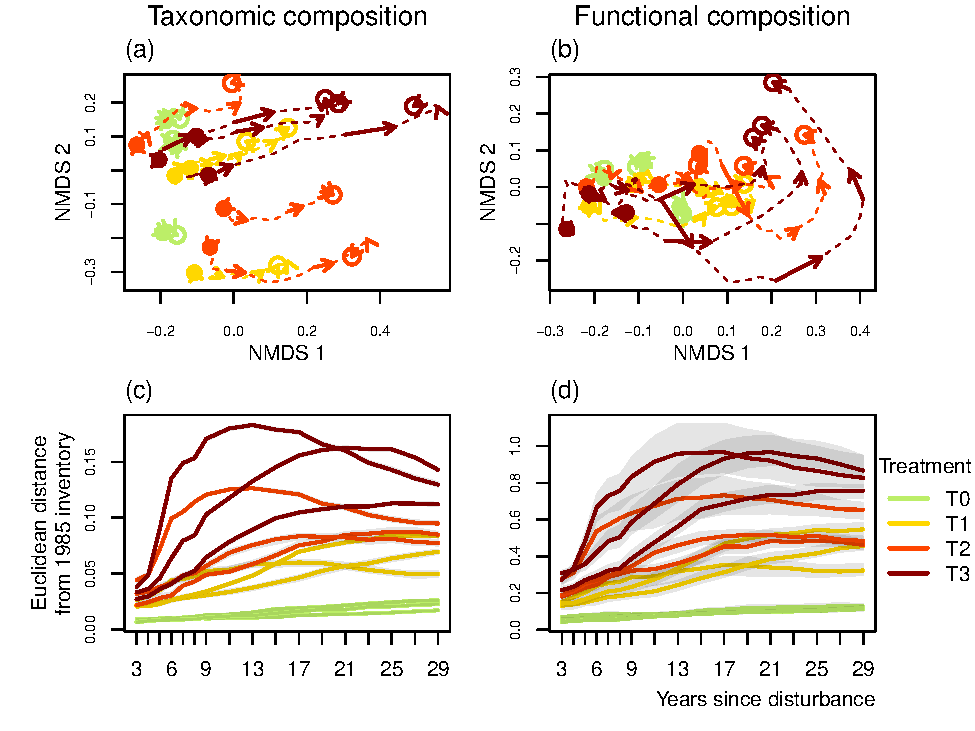
\includegraphics[width=1\linewidth]{Manuscript_files/figure-latex/NMDSplans-1} 

}

\caption{Plot trajectories in terms of flora composition (left panels \textbf{(a)} and \textbf{(c)}) and functional composition (right panels \textbf{(b)} and \textbf{(d)}) in a two-dimensional NMDS space. Lower panels (\textbf{(c)} and \textbf{(d)}) represent the Euclidean distance to initial condition along the 30 sampled years. Shaded areas are the credibility intervals.}\label{fig:NMDSplans}
\end{figure*}

Except for leaf chlorophyll content, which continued to increase for
some T3 and T2 plots 30 years after disturbance, all traits and seed
mass proportions followed unimodal trajectories either stabilizing or
returning towards their initial values.

Maximum height at adult stage (\emph{Hmax}), leaf toughness and wood
specific gravity (\emph{WSG}) first decreased and then slightly
increased but remained significantly lower than their initial value
(Fig. \ref{fig:CWM}). On the other side, bark thickness and specific
leaf area (\emph{SLA}) increased and while bark thickness remained
substantially high after 30 years, \emph{SLA} had almost recovered its
initial value. For all traits, the maximum difference to initial value
was correlated to the disturbance intensity
(\(\rho_{spearman}^{Leaf thickness}=0.76\),
\(\rho_{spearman}^{Chlorophyll content}=0.60\),
\(\rho_{spearman}^{Leaf toughness}=-0.53\),
\(\rho_{spearman}^{SLA}=0.93\), \(\rho_{spearman}^{WSG}=-0.75\),
\(\rho_{spearman}^{Bark thickness}=0.71\),
\(\rho_{spearman}^{Hmax}=-0.40\)). The proportions of the three lightest
seed mass classes increased in all disturbed plots, and decreased after
30 years for the lightest class while it stabilized for the two other
(Supp. Mat. - Fig. S2).

\begin{figure*}

{\centering 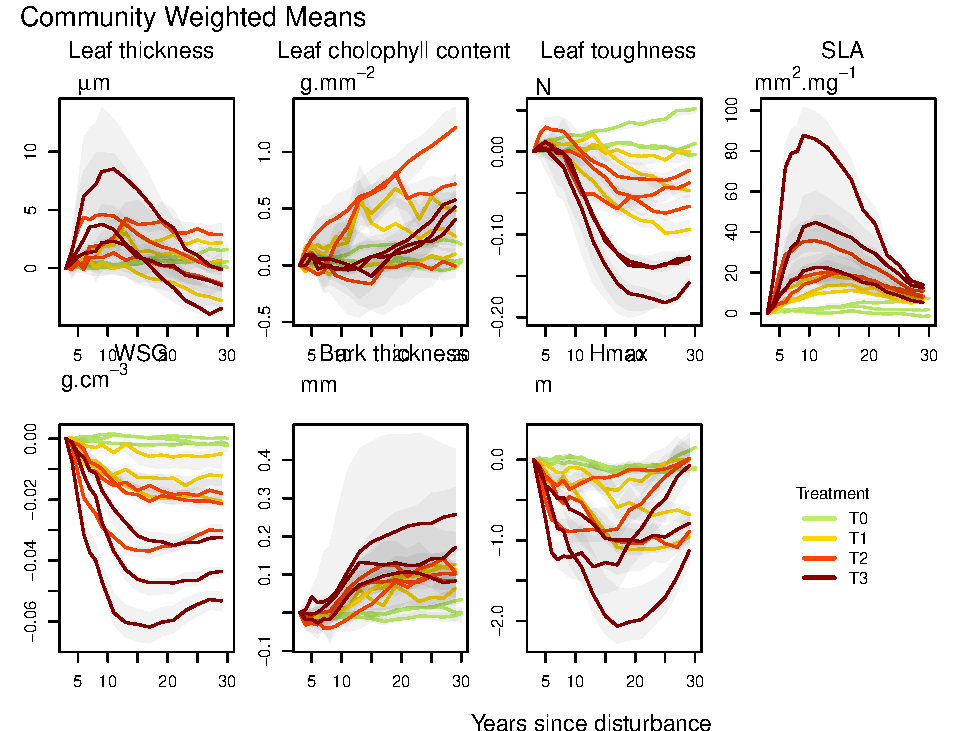
\includegraphics[width=1\linewidth]{Manuscript_files/figure-latex/CWM-1} 

}

\caption{Trajectories of the communities weighted means over 30 years after disturbance of four leaf traits (Leaf thickness, chlorophyll content, toughness, and specific area), two stem traits (wood specific gravity, and bark thickness) and one life history trait (Specific maximum height at adult stage). }\label{fig:CWM}
\end{figure*}

\subsubsection{Communities richness and
evenness}\label{communities-richness-and-evenness}

For undisturbed plots, taxonomic Richness and Evenness remained stable
over the 30 years monitored. In disturbed communities, after low
disturbance intensity the taxonomic richness increased, reaching a
maximum gain of 14 botanical genera (plot 3 from treatment 2). After
intense disturbance the taxonomic richness followed a more complex
trajectory, decreasing for ten years after disturbance before recovering
to pre-disturbance values. The maximum richness loss or gain after
disturbance was positively correlated to the disturbance intensity
(\(\rho_{spearman}^{Richness}=0.50\)). In all disturbed plots the
taxonomic evenness first increased until a maximum reached after around
20 years. This maximum was positively correlated to the disturbance
intensity (\(\rho_{spearman}^{Evenness}=0.77\)). The evenness then
stabilized except for two T3 plots (plots 8 and 12) for which evenness
kept increasing.

\begin{figure*}

{\centering 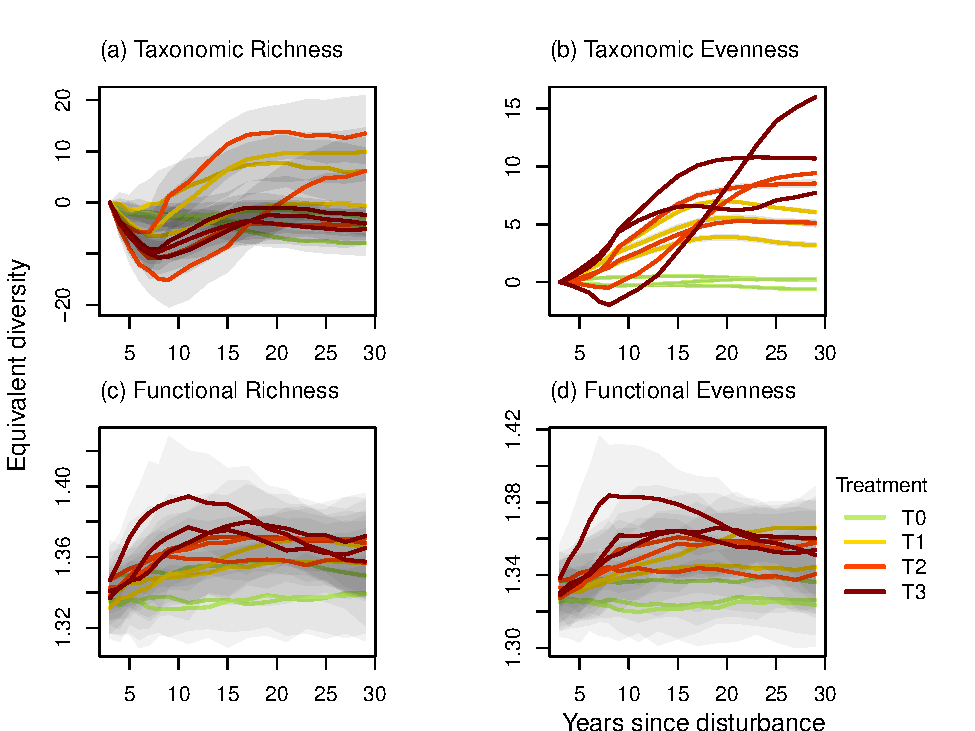
\includegraphics[width=1\linewidth]{Manuscript_files/figure-latex/DivTaxo-1} 

}

\caption{Trajectories over 30 years of the difference with the 1989 inventory (2 years after disturbance) of community taxonomic \textbf{(a)} richness, \textbf{(b)}, taxonomic evenness, \textbf{(c)} functional richness, and \textbf{(d)} functional evenness. Shaded areas are the credibility intervals }\label{fig:DivTaxo}
\end{figure*}

The plot 7 from treatment 1 displayed constantly outlying functional
richness and evenness and was removed from the graphical representation
for better readability. In undisturbed plots both functional richness
and evenness remained stable along the 30 years. In disturbed plots,
functional richness and evenness trajectories depended on the
disturbance intensity with their maximum positively correlated to \%AGB
loss \(\rho_{spearman}^{Richness}=0.76\) and
\(\rho_{spearman}^{Evenness}=0.60\). Functional richness and evenness
displayed for low disturbance intensity a low but long-lasting increase
up to a maximum reached after 20-25 years, and for high intensity, a
fast but short increase followed after 10 years by a slow decrease
towards the initial values.

The second-degree polynomial regressions between (i) the percentage AGB
loss and (ii) taxonomic and functional richness and evenness after 10,
20 and 30 years best predicted the hump-shaped curve of the disturbance
impact along the disturbance intensity gradient \ref{fig:IDHplot}. The
relationship between the disturbance impact and its intensity was more
markedly hump-shaped for the taxonomic richness than for the taxonomic
evenness. For both functional richness and evenness the relationship was
almost linear. The regression model better predicted the functional
richness and evenness (\(0.55<R^2_{Functional Richness}<0.72\), and
\(0.60<R^2_{Functional Evenness}<0.81\)) than the taxonomic richness and
evenness (\(0.21<R^2_{Taxonomic Richness}<0.4\), and
\(-0.15<R^2_{Taxonomic Evenness}<0.43\) respectively)

\begin{figure*}

{\centering 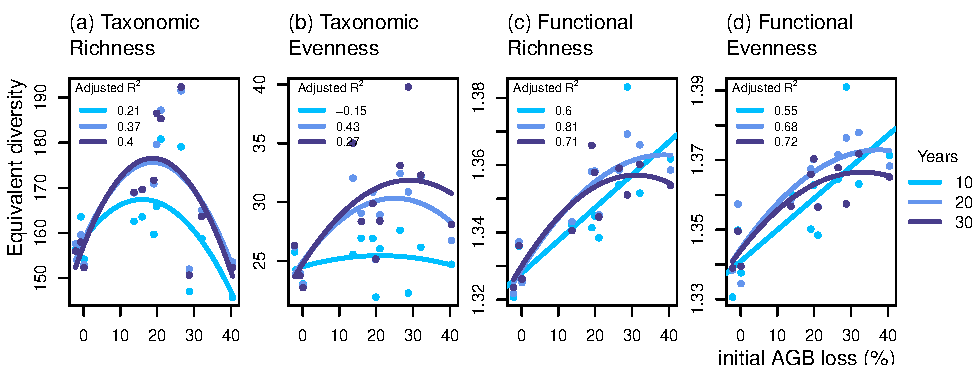
\includegraphics[width=1\linewidth]{Manuscript_files/figure-latex/IDHplot-1} 

}

\caption{Relationship between the initial \%AGB loss and community taxonomic richness \textbf{(a)}, taxonomic evenness \textbf{(b)}, functional richness \textbf{(c)},and functional evenness \textbf{(d)} at 10, 20 and 30 years after disturbance}\label{fig:IDHplot}
\end{figure*}

\subsubsection{Functional redundancy}\label{functional-redundancy}

All disturbed plots had lower functional redundancy than control plots
and followed similar hump-shaped trajectories (\ref{fig:RedFunRest}).
The maximum redundancy loss was positively correlated with the
disturbance intensity (\(\rho_{spearman}=0.47\)) and the initial value
had not recovered for any disturbed communities after 30 years.

\begin{figure}

{\centering 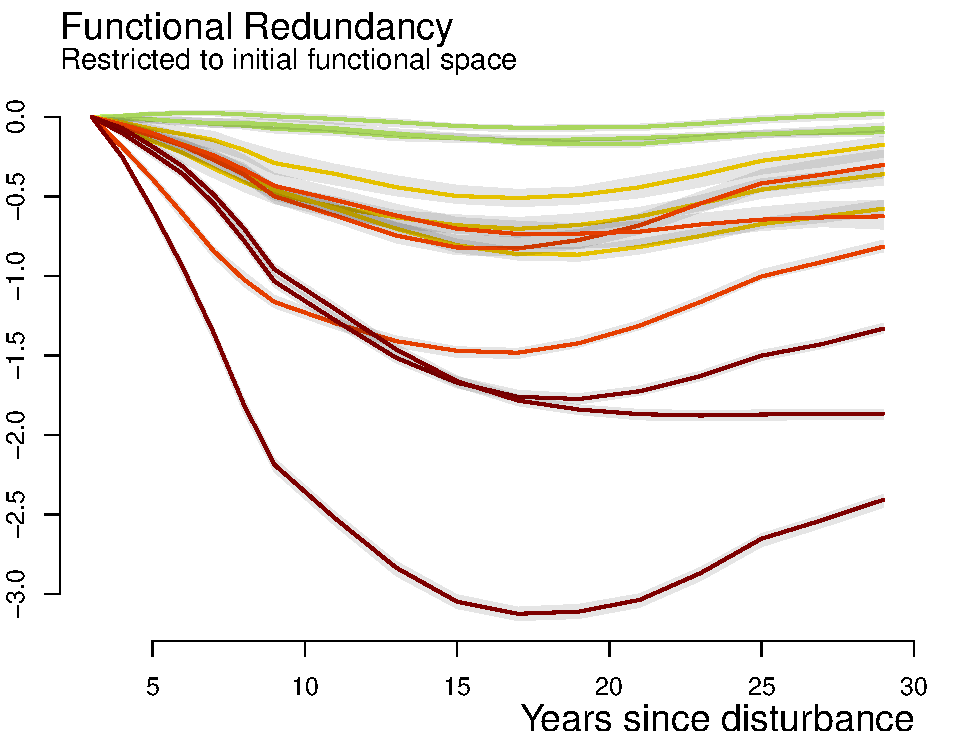
\includegraphics[width=0.8\linewidth]{Manuscript_files/figure-latex/RedFunRest-1} 

}

\caption{Trajectories of the functional redundancy within the initial functional space over 30 years after disturbance. Shaded areas are the credibility intervals.}\label{fig:RedFunRest}
\end{figure}

\subsection{Discussion}\label{discussion-1}

\subsubsection{A cyclic recovery of community
composition}\label{a-cyclic-recovery-of-community-composition}

Community taxonomic and functional composition appeared resilient,
following similar hump-shaped trajectories starting to return towards
pre-disturbance composition after 30 years.

The taxonomic differences among local communities, marked before
disturbance by the distinct starting points on the NMDS axis 2, were
maintained throughout recovery trajectories. More than commonly thought,
post-disturbance trajectories depended on community initial composition,
that partly determined the pool of recruited species and constrained the
trajectories towards the initial composition. The high resilience of
community taxonomy, in the sense of the initial state recovery, revealed
that species not belonging to the pre-disturbance community were hardly
recruited because of the commonness of dispersal limitation among
tropical tree species \autocite{Svenning2005}.

Conversely, disturbed communities followed functional trajectories that
are highly similar in terms of functional composition. As
pre-disturbance surviving trees mirror the initial community
\autocite{Herault2018}, changes in functional composition relied upon
the recruitment of species or functional types that were infrequent or
absent before disturbance. Competitive pioneers became dominant in
filling the environmental niches of high availability of light, space
and nutrients vacated by the disturbance. The recruitment of pioneers
changed community functional composition in the same way for all
disturbance intensity towards more resource-acquisitive strategies,
moving community functional composition right along the first axis in
Fig. \ref{fig:NMDSplans} \autocites{Westoby1998}{Wright2004}{Reich2014}.
Thereafter long-lived, more resistant and shade-tolerant species
excluded the first established pioneers and started the recovery of
pre-disturbance functional composition, moving similarly community
functional composition left along the first axis and upward along the
second axis in Fig. \ref{fig:NMDSplans}.

These trajectories provided empirical support to the hypothesis that
community assembly is both deterministic and historically convergent at
different levels of community organization. Deterministic, trait-based
processes drove community convergence in functional composition, while
at the same time dispersal limitation maintained their divergence in
taxonomic composition \autocite{Fukami2005}.

\subsubsection{Another perspective on the intermediate disturbance
hypothesis}\label{another-perspective-on-the-intermediate-disturbance-hypothesis}

The IDH well predicted well the disturbance impact on community
taxonomic richness, enhanced until an intensity threshold (20-25\% AGB
loss), and to some extent on taxonomic evenness, somewhat decoupled from
the disturbance intensity as already observed in the Guiana Shield
\autocite{Baraloto2012a} and in Bornean tropical forests
\autocite{Cannon1998}. The disturbance intensity determined the balance
in the community between pre-disturbance surviving trees and those
recruited afterward. The pool of true pioneer species specifically
recruited after disturbance is restricted in the Guiana Shield to a few
common genera (e.g.~Cecropia spp., Vismia spp.) \autocite{Guitet2018}.
Below the intensity threshold the size of the surviving community
maintained the pre-disturbance high taxonomic richness while the
recruitment of pioneers, infrequent or absent before disturbance,
increased both community taxonomic richness and evenness. Beyond the
intensity threshold, the disturbance decreased the taxonomic richness of
surviving trees which was not offset by the enrichment of pioneers, so
that the overall community taxonomic richness decreased according to the
disturbance intensity \autocite{Molino2001}. For community taxonomic
evenness the disturbance impact was similar but slighter, as the
evenness is less sensitive to the loss of rare species. Taxonomic
evenness rather represented the increasing dominance of pioneers that
balanced the usual hyper-dominance of a few species in tropical forests
below the intensity threshold, thus increasing community overall
evenness up to the intensity threshold beyond which pioneers became in
turn highly dominant and decreased the overall evenness
\autocite{Baraloto2012a}.

Conversely the IDH was disproved regarding the disturbance impact on
community functional richness and evenness. Irrespective of the
disturbance intensity the recruitment of pioneers, functionally highly
different from the composition of pre-disturbance community, increased
both community functional richness and evenness.

Along time, taxonomic richness trajectories of all disturbed communities
first dropped similarly, following the species loss due to disturbance,
and then displayed a species gain depending on the disturbance
intensity. Up to an intensity threshold, the species gain was all the
more significant that the disturbance intensity increased, with the
establishment of long-lived pioneers enhancing community taxonomic
richness and evenness in the long term. These long-lived pioneers,
functionally quite different from the functional composition, entailed
as well a progressive and long-lasting increase of the functional
richness and evenness \autocites{Denslow1980}{Molino2001}. Beyond an
intensity threshold, though, a few short-lived pioneers occupied the
vacated environmental space and prevented the establishment of other
species. These short-lived pioneers were functionally very different
from the pre-disturbance community and entailed a rapid and significant
increase of functional richness and evenness. Already after 10 years,
though, short-lived pioneers started to decline and the functional
richness and evenness decreased. Likely this decrease will be followed
by the establishment of long-lasting pioneers, and by the time they
recruit we expect the taxonomic and functional trajectories to catch up
with those observed after intermediate disturbance
\autocite{Walker2009}.

\subsubsection{The functional redundancy, key of community
resilience}\label{the-functional-redundancy-key-of-community-resilience}

For 15 years the species loss during disturbance, determined by the
disturbance intensity, commensurately decreased the functional
redundancy within the pre-disturbance functional space. The redundancy
decrease was not compensated in the first place as the first recruited
pioneers were functionally different from the pre-disturbance functional
composition. Progressively though, first established species were
replaced by more competitive long-lived pioneers or late-successional
species resembling more the pre-disturbance functional composition and
restoring the functional redundancy. This replacement was stochastic and
followed the lottery recruitment rules, implying a recruitment eased for
the first recruited species but then increasingly hampered by the
emergence of interspecific competition \autocite{Busing2002}. Along time
the recovery of infrequent species was increasingly slow, so that the
time for the full recovery of the functional redundancy, in some
communities just initiated after 30 years, was extremely difficult to
estimate \autocites{Elmqvist2003}{Diaz2005}.

The long-term impact of disturbance on community functional redundancy
meant a lower resilience of the pre-disturbance communities, with higher
chances to see the persistence of disturbance-specific species at the
expense of late-successional ones \autocite{Haddad2008}. Besides, the
long-term recovery of infrequent species increases the risks to loose
cornerstone species, with unexpected ecological consequences
\autocites{Jones1994}{Chazdon2003a}{Diaz2005}. Apart from the functional
characteristics considered here, infrequent species might indeed have
unique functions in the ecosystem or be a key for some fauna
\autocite{Schleuning2016}.

\subsection{Conclusions}\label{conclusions}

Our study revealed community recovery through the combination of
deterministic processes driving their convergence in functional
composition, and dispersal limitation maintaining their divergence in
taxonomic composition. The IDH was validated for community taxonomic
richness and, to some extent, taxonomic evenness but disproved regarding
community functional richness and evenness that were enhanced for any
disturbance intensity by the high functional differences of pioneers
compared to late-successional functional composition. The IDH was
translated in time by the recruitment, beyond an intensity threshold, of
short-lived pioneers that prevented in the first times the establishment
of more diverse long-lived pioneers, recruited otherwise below the
intensity threshold. The resilience of tropical forests, in the sense of
the pre-disturbance state recovery, proved tangible but requiring
several decades. Still, the disturbance impact on communities redundancy
cautioned against the risks of infrequent species loss and the
persistence of disturbance-specific communities \autocite{Herault2018}.

\subsection{Acknowledgement}\label{acknowledgement}

We are in debt with all technicians and colleagues who helped setting up
the plots and collecting data over years. Without their precious work,
this study would have not been possible and they may be warmly thanked
here.

\subsection{Author's contributions}\label{authors-contributions}

AM, EM \& BH designed the study, developed the analysis framework,
interpreted the results and wrote the manuscript. All authors gave final
approval for publication.

\subsection{Data availability}\label{data-availability}

This article is based upon the dataset of the Paracou station, which is
part of the Guyafor permanent plot network in French Guiana
(Cirad-CNRS-ONF). The dataset is available upon request to the
scientific director (\url{https://paracou.cirad}. fr).

\chapter{Analyse du recrutement, support de la trajectoire des
communautés}\label{analyse-du-recrutement-support-de-la-trajectoire-des-communautes}

La réponse des communautés aux perturbations est déterminée par les
trajetoires du recrutment, reconnu pour suivre une succession
déterministe régie après perturbation. Ceci reste cependant à tester
dans le cas des forêts tropicales, dont l'immense biodiversité pourrait
atténuer les processus déterministes, et dans le cas particulier de
perturbations relativement peu intenses en comparaison des coupes rases
ou de la secondarisation pour lesquels ont été observés les modèles de
succession classique.\\
Nous étudions dans ce chapitre les trajectoires de diversité taxonomique
et fonctionnelle du recrutement après exploitation pour (i) clarifier
l'importance respective des processus stochastiques et déterministes au
cours de la succession des processus écologiques et (ii) déterminer la
résilience et la durée de restauration des processus démographiques
après exploitation.

Nous avons tracé les trajectoires de diversité et d'équitabilité
taxonomique et fonctionnelle, et de renouvellement des espèces par
rapport à la communauté initiale. Nous avons ensuite comparé ces
trajectoires à celles de modèles nuls stochastiques.

Nous avons identifié trois phases de recrutement après perturbation,
définies par la combinaison de processus déterministes et stochastiques.
La première phase de succession correspond à la croissance de juvéniles
recrutés aléatoirement dans la communauté initiale. La deuxième phase
correspond à l'émergence de processus déterministes favorisant le
recrutement de pionnières issues de la banque de graines. La troisième
et dernière phase correspond à la restauration des processus de
recrutement aléatoire entraînant un retour de la diversité et de la
composition initiales. Malgré la rapide restauration des processus de
recrutement, la restauration de la composition et de la diversité du
recrutement s'est montrée longue de plusieurs décennies.

La trajectoire des communautés après perturbation est déterminée par
l'émergence de processus de recrutement déterministes favorisant les
espèces héliophiles, remplaçant temporairement le recrutement
stochastique propre aux communautés matures. Bien que résilientes les
caractéristiques taxonomiques et fonctionnelles du recrutement se sont
montrée impactées sur plusieurs décennies, incitant à la prudence quand
au maintien des caractéristiques initiales.

\newpage

\section{30 Years of Post-disturbance Recruitment in a Neotropical
Forest}\label{years-of-post-disturbance-recruitment-in-a-neotropical-forest}

Ariane MIRABEL \textsuperscript{1} \textsuperscript{*}

Eric Marcon \textsuperscript{1}

Bruno Hérault \textsuperscript{2} \newline

\textsuperscript{1} UMR EcoFoG, AgroParistech, CNRS, Cirad, INRA,
Université des Antilles, Université de Guyane. Campus Agronomique, 97310
Kourou, France.

\textsuperscript{2} INPHB, Institut National Polytechnique Félix
Houphoüet-Boigny Yamoussoukro, Ivory Coast. \newline

* E-mail:
\href{mailto:ariane.mirabel@ecofog.gf}{\nolinkurl{ariane.mirabel@ecofog.gf}},
url: \url{https://github.com/ArianeMirabel} \#\#\# Abstract

The role of tree diversity for tropical forests functioning and services
makes it crucial tree diversity and composition fate in the global
changing context. Community long-term response to disturbance rely on
tree recruitment, long seen as following deterministic successional
pathways. These pathways however might be altered in the hyper-diverse
tropical forests and of slight but recurrent disturbances induced by
global changes. Post-disturbance recruitment trajectories would (i)
disentangle the determinants of tree recruitment between stochastic and
deterministic processes that enhance a restricted pool of species, and
(ii) elucidate tropical forests taxonomic and functional resilience. We
examined the trajectories over 30 years of recruited trees taxonomic and
functional diversity in 75 ha of forest following a disturbance
gradient. We analyzed taxonomic richness, evenness, and turnover, and
functional diversity and composition (regarding 7 leaf, stem and
life-history functional traits). We highlighted a three-phased
successional pathway defined by the interplay of stochastic and
deterministic recruitment processes. The succession translated into (i)
saplings growth mirroring pre-disturbance communities, (ii)
light-demanding species enhanced recruitment entailing, above a
disturbance intensity threshold, the dominance of pioneers and (iii) the
recovery of pre-disturbance taxonomic and functional characteristics and
of stochastic recruitment processes. Although tangible, community
taxonomic and functional resilience was decades-long.

Post-disturbance recruitment relied on deterministic competition
processes for light balancing the stochastic processes ruling
undisturbed communities. Although resilient, recruitment taxonomic and
functional characteristics remained altered in the long-term, calling
caution for forest management.

\textbf{Keywords}: Disturbance Dynamics, Neotropical Forests,
Recruitment, Resilience, Taxonomic and Functional Diversity, Tree
Community

\subsection{Introduction}\label{introduction-2}

Determining the response of tropical forests to disturbance is key to
predict their fate in the global changing context. In the last decades,
tropical forests experienced a wide range of disturbance, from radical
land-use changes for agriculture or mining
\autocites{Dezecache2017a}{Dezecache2017b} to more insidious changes of
communities structure, diversity and functioning following climatic
changes \autocite{Aubry-Kientz2015} or anthropogenic activities like
selective logging \autocite{Baraloto2012a}. In that respect a vast
literature successfully modeled community response to disturbance in
terms of tree growth, tree height and fluxes of carbon, water and
nutrients
\autocites{Gourlet-Fleury2000}{Putz2012}{Piponiot2016}{Rutishauser2016}.
Similar modeling approaches regarding forest diversity and composition
remain hindered by the scarcity of long-term monitoring and by studies'
restriction to common or commercial species imposed by forest huge
biological diversity \autocites{Sebbenn2008}{Vinson2015}. The template
of community response to disturbance is set by recruitment processes
that determine the new species joining the community. Focusing on
long-term recruitment trajectories therefore give valuable insight into
post-disturbance recovery and hence into the adjustment of exploitation
and conservation guidelines \autocites{Diaz2005}{Schwartz2017}.

The traditional view of community response to disturbance relies on
successional vegetation models \autocite{Clements1916} based on changes
in resources availability and interactions among species. Adapted to
forest ecosystems the successional framework translates into
\autocite{Denslow2000} (i) the recruitment of pre-disturbance surviving
saplings benefiting from the high resources availability and low
competition, (ii) the progressive exclusion of species with low
competitive ability because of increased competition for resources
following stand maturation and (iii) the recovery of pre-disturbance
composition and diversity due to the senescence of early-successional
pioneers and the emergence of late-successional species. This
highly-deterministic successional pathway proved relevant in temperate
forests but remain questioned in tropical rainforests
\autocite{Norden2015}. Indeed, the classical successional pathway may be
altered by the huge biological diversity of tropical rainforests and
their high functional redundancy that lead up to more stochastic
processes. Moreover, the successional pathway proved well-adapted to
system trajectories following clear cutting or very intense disturbance,
but might be less robust following more insidious global changes. In
those cases, community trajectories would depend on the interplay
between the stochastic processes, driven by recruitment and dispersal
limitations \autocite{Hubbell2001}, and deterministic processes, driven
by niche-based competition and biotic interactions \autocite{Adler2007}.
Stochastic processes, in the neutral theory spirit, build recruited
communities as random samples of the surrounding communities
\autocites{Hubbell2001}{Chave2004}. In contrast under deterministic
processes, species are selected with respect to their ecological
strategies and competitive ability. The relative importance of
stochastic and deterministic processes in shaping the post-disturbance
trajectories would also change with time, along with the recovery of
pre-disturbance environmental conditions.

The processes shaping recruitment trajectories may differently affect
communities taxonomic characteristics, that refer to neutral species
assemblages, and functional characteristics, that account for species
ecology and ecosystem functioning \autocites{Violle2007b}{Kunstler2016}.
The correlations, or not, between community taxonomic and functional
trajectories are therefore insightful of the main ecological processes
underlying species recruitment \autocite{Fukami2005}. Among these
processes, competition depends on the species competitive ability for a
given niche, defined by the functional differences regarding the use of
limited shared resources \autocite{Perronne2017}. In tropical forests
where light is the limiting resource, community response to disturbance
would translate in a shift from slow-growing, long-lived species with
``conservative'' resource use, to fast-growing species with
``acquisitive'' resource use
\autocites{Denslow1980}{Molino2001}{Bongers2009}.\\
The competition processes at stake would be grasped by shifts in key
leaf, wood and life-history functional traits assessing species
resources acquisition strategy and ecology
\autocites{Wright2004}{Chave2009b}{Herault2011}.

Balancing between determinism and stochasticity, post-disturbance
recruitment trajectories might thus show either a random divergence or a
deterministic convergence towards stable taxonomic and functional
characteristics, likely defined by the environment
\autocites{Clements1916}{Diamond1975}. Both views were reconciled under
the hypothesis that communities might diverge in the taxonomic space,
having different taxonomic composition and diversity, while they
converge in the functional space, but this remains to be tested in
tropical forests \autocites{Fukami2005}{Li2018}.

In this paper we followed recruitment trajectories over 30 years of 75
ha of Neotropical forest plots set up on a gradient of disturbance
intensity, from 10 to 60\% of forest biomass removed. We examined the
recruited trees (i) taxonomic composition, richness and evenness, (ii)
taxonomic turnover compared to pre-disturbance community, and (iii)
functional composition and diversity based on seven major leaf, stem and
life-history traits. We compared the recruitment trajectories to neutral
models corresponding to a stochastic recruitment and a randomization of
species functional traits. Specifically, we (i) elucidated the
successional pathway shaping community response to disturbance and the
underlying ecological processes and (ii) clarified the extent of
community taxonomic and functional resilience,in the sense of
pre-disturbance characteristics recovery, and its consequences for
tropical forest management.

\subsection{Material and Methods}\label{material-and-methods-1}

\subsubsection{Study Site}\label{study-site-1}

The Paracou station is located in a lowland tropical rainforest in
French Guiana (518\textdegree N and 5253\textdegree W). Climate is
tropical wet with mean annual precipitation averaging 2980
mm.yr\textsuperscript{-1} (30-yr period) and a 3-months dry season
(\textless{} 100 mm.mo\textsuperscript{-1}) from mid-August to
mid-November, and a one-month dry season in March \autocite{Wagner2011}.
Elevation ranges from 5 to 50 m and mean annual temperature is
26\textdegree C. Soils are thin acrisols over a layer of transformed
saprolite with low permeability generating lateral drainage during heavy
rains. The experiment is a network of twelve 6.25 ha plots (Table
\ref{tab:Tab1bis}) that underwent three disturbance treatments in 1987
according to a randomized plot design with three replicate blocks of
four plots \autocite{Herault2018}.

\begin{longtable}[t]{l|l|l|l|l}
\caption{\label{tab:Tab1bis}Intervention table, summary of the disturbance intensity for the 4 plot treatments in Paracou.}\\
\hline
Treatment & Timber & Thinning & Fuelwood & \%AGB lost\\
\hline
Control & - & - & - & 0\\
\hline
T1 & DBH $\geq$ 50 cm, commercial species, $\approx$ 10   $trees.ha^{-1}$ & - & - & $[12-33]$\\
\hline
T2 & DBH $\geq$ 50 cm, commercial species, $\approx$ 10  $trees.ha^{-1}$ & DBH $\geq$ 40 cm, non-valuable species, $\approx$ 30   $trees.ha^{-1}$ & - & $[33-56]$\\
\hline
T3 & DBH $\geq$ 50 cm, commercial species, $\approx$ 10  $trees.ha^{-1}$ & DBH $\geq$ 50 cm, non-valuable species, $\approx$ 15  $trees.ha^{-1}$ & 40 cm $\leq$ DBH $\leq$ 50 cm, non-valuable species,\ $\approx$ 15 $trees.ha^{-1}$ & $[35-56]$\\
\hline
\end{longtable}

\subsubsection{Inventories Protocol and Dataset
Collection}\label{inventories-protocol-and-dataset-collection-1}

Dominant families in the study site are Fabaceae, Chrysobalanaceae,
Lecythidaceae and Sapotaceae. All trees above 10 cm DBH were mapped and
measured annually since 1984. Trees are first identified with a
vernacular name assigned by the forest worker team, and afterward with a
scientific name assigned by botanists during regular botanical
campaigns. Botanical campaigns have been carried out every five to six
years from 2003 onwards but identification levels varied between
campaigns.

These variability of protocols in time raised methodological issues as
vernacular names usually correspond to different botanical species. It
resulted in significant taxonomic uncertainties that had to be
propagated to composition and diversity metrics. The uncertainty
propagation was done through a Bayesian framework reconstituting
complete inventories at genus level from real incomplete ones on the
basis of vernacular/botanical names association. Vernacular names were
replaced through multinomial trials based on the association probability
\(\big[\alpha_1, \alpha_2,..., \alpha_N\big]\) observed across all
inventories between each vernacular name \emph{v} and the species
\(\big[s_1, s_2,..., s_N\big]\):

\begin{align}
M_v\Big(\big[s_1, s_2,..., s_N\big],\big[\alpha_1, \alpha_2,..., \alpha_N\big]\Big) \nonumber
\end{align}

See appendix 1 and \textcite{Aubry-Kientz2013} for the detailed
methodology.

To minimize the remaining identification uncertainties, the simulated
botanical inventories were reported at genus level.

Six functional traits representing the leaf economics (leaves thickness,
toughness, total chlorophyll content and specific leaf area) and stem
economics spectra (wood specific gravity and bark thickness), and
life-history traits (maximum specific height and seed mass) were
considered. Traits were extracted from the BRIDGE project
(\url{http://www.ecofog.gf/Bridge/}) where trait values were assessed
from a selection of individuals located in nine permanent plots in
French Guiana, including two in Paracou, and comprised 294 species
pertaining to 157 genera. Missing trait values (10\%) were filled by
multivariate imputation by chained equation \autocite{Mice2011}.
Imputations were restricted within genus or family when samples were too
scarce, in order to account for the phylogenetic signal.\\
As seed mass information was classified into classes, no data filling
process was applied and analyses were restricted to the 414 botanical
species recorded.

All composition and diversity metrics were obtained after 50 iterations
of the uncertainty propagation framework.

\subsubsection{Recruitment trajectories}\label{recruitment-trajectories}

Communities were split into surviving trees of pre-disturbance
communities and trees recruited afterward in 2-years intervals.

Taxonomic diversity trajectories were assessed through species richness
and evenness (the Hill number translation of the Simpson index)
\autocites{Chao2015}{Marcon2015b}.\\
The two diversities belong to the set of HCDT or generalized entropy,
respectively corresponding to the zero and two order of diversity
(\emph{q}), which grasps the balance between richness and evenness in
the community through the value of \emph{q} that emphasizes common
species.

Functional diversity trajectories were assessed through the Rao index of
quadratic entropy, which combines species abundance distribution and
average pairwise dissimilarity based on all functional traits.
Functional composition trajectories were assessed through the functional
traits community weighted means (CWM), representing the average trait
value in a community weighted by species relative abundance
\autocite{Diaz2007}. Seed mass trajectories were reported by the
proportion of each class recorded in the inventories.

The taxonomic similarity between recruited trees and pre-disturbance
forest was measured with the turnover metrics detailed in
\textcite{Podani2013a}.

The taxonomic and functional recruitment trajectories were compared to
null trajectories obtained after 50 iterations of the null models. The
taxonomic null model was a random sampling of recruited trees within the
living communities, with the maintenance of species abundance and tree
density. The functional null model was a reassignment of species trait
values that randomized traits abundances but maintained communities
abundance distribution \autocite{Mason2013}. The null trajectories were
similarly obtained after 50 iterations of the random sampling.

\subsection{Results}\label{results-2}

\subsubsection{Taxonomic richness and evenness and functional
diversity}\label{taxonomic-richness-and-evenness-and-functional-diversity}

In undisturbed communities the recruitment taxonomic richness and
evenness remained stable over the 30 years and with values equivalent to
those of the taxonomic null model (Figure (\ref{fig:DivTraj})).

In disturbed communities the taxonomic richness followed hump-shaped
trajectories first increasing until a maximum reached after around 15
years and positively correlated to the disturbance intensity
(\(\rho^{Richness}_{spearman}=0.93\)). Afterward the taxonomic richness
decreased and recovered the pre-disturbance values after 30 years. The
observed taxonomic richness was increasingly lower than this of null
model for 15 years, then the difference started to shrink but the
observed richness remained negative remained negative until after 30
years. The taxonomic evenness decreased independently of the disturbance
intensity over the 30 years (\(\rho^{simpson}_{spearman}=-0.35\)). The
observed taxonomic eveness was increasingly lower than this of the null
model until 15 years after disturbance, when the difference stabilized.

The functional diversity in the undisturbed plots remained stable and
equivalent to this of the functional null model over the 30 years. In
the lowest disturbance plots the functional diversity remained stable or
slightly increasing, and was higher than this of the null model for two
of the T1 plots. In the disturbed plots of higher disturbance intensity
(T2 and T3) the functional diversity decreased until 15 years after
disturbance, when it started to recover towards initial values. The
observed functional diversity remained lower than this of the null model
over the 30 years.

\begin{figure*}

{\centering 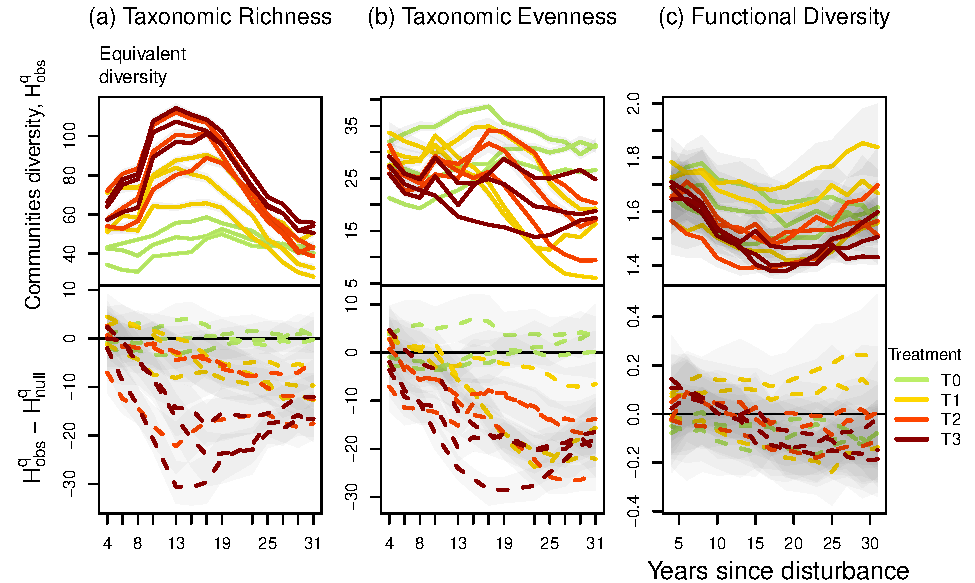
\includegraphics[width=1\linewidth]{Manuscript_files/figure-latex/DivTraj-1} 

}

\caption{Upper panels, trajectories over 30 years of taxonomic richness \textbf{(a)}, taxonomic evenness \textbf{(b)} and functional diversity \textbf{(c)} of observed 2-years laps recruitment $H_{obs}^q$. Lower panels, diversity differences to null models $H_{obs}^q - H_{null}^q$}\label{fig:DivTraj}
\end{figure*}

\subsubsection{Functional composition}\label{functional-composition}

In undisturbed plots functional traits values remained stable over the
30 years while it followed hump-shaped trajectories in all disturbed
plots, to the exception of the leaf chlorophyll content. Trajectories of
SLA and bark thickness first increased before decreasing towards initial
values. Conversely, trajectories of leaf thickness, leaf toughness, wood
specific gravity, and maximum height first decreased and then started
returning towards initial values but their recovery remained unachieved
after 30 years (Figure \ref{fig:CWMbis}).

\begin{figure*}

{\centering 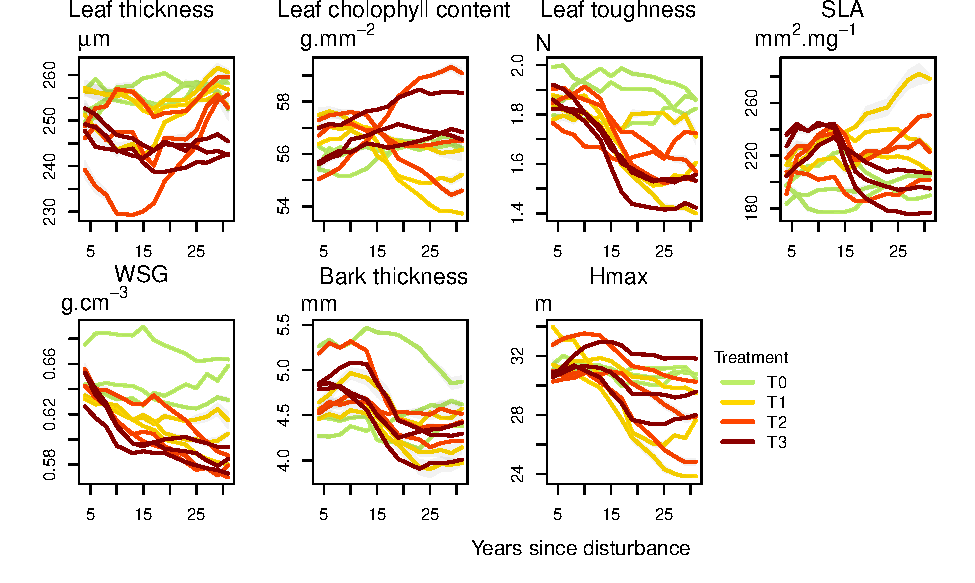
\includegraphics[width=1\linewidth]{Manuscript_files/figure-latex/CWMbis-1} 

}

\caption{Community weighted means (CWM) of the leaf, the two stem and specific maximum height. Shaded areas are the credibility intervals.}\label{fig:CWMbis}
\end{figure*}

\subsubsection{Recruitment Turnover}\label{recruitment-turnover}

Over the 30 years in control plots the turnover of recruited species
compared to initial community remained low (Figure \ref{fig:Turnover}).
In disturbed plots the recruited species turnover followed a marked
hump-shaped trajectory, with a maximum reached around 15 years after
disturbance. The maximum turnover was positively correlated to the
disturbance intensity (\(\rho_{spearman}=0.93\)). Thirty years after
disturbance the turnover had returned to low values.

\begin{figure*}

{\centering 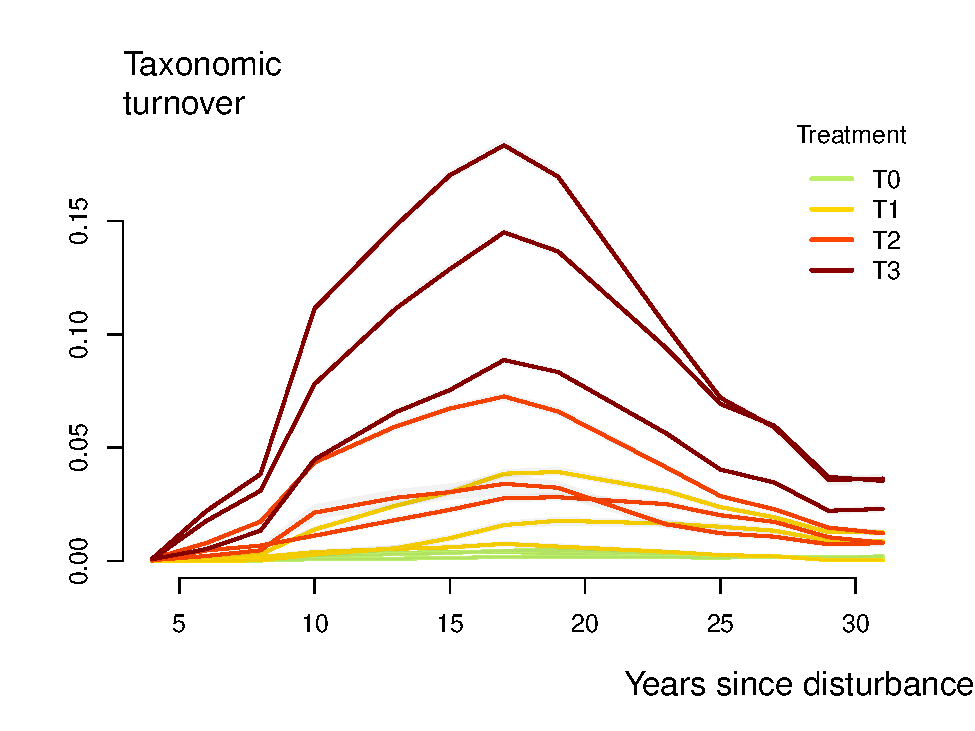
\includegraphics[width=1\linewidth]{Manuscript_files/figure-latex/Turnover-1} 

}

\caption{Trajectories over 30 years of the abundance-based turnover between 2-years laps recruited trees pre-disturbance communities.}\label{fig:Turnover}
\end{figure*}

\subsection{Discussion}\label{discussion-2}

\subsubsection{A three-phased deterministic successional
pathway}\label{a-three-phased-deterministic-successional-pathway}

Post-disturbance recruitment trajectories relied on a three-phased
successional pathway defined by the emergence of deterministic
competition processes for light gradually balancing the stochastic
recruitment specific to undisturbed communities.

A first phase (0-8 years), corresponded to the recruitment of
pre-disturbance surviving saplings (DBH \textless{} 10 cm) that
immediately benefited from the increased enlightment and alleviated
competition induced by disturbance \autocites{Denslow2000}{Herault2010}.
The taxonomic and functional characteristics of recruited trees mirrored
the pre-disturbance communities and recruitment processes matched the
null stochastic recruitment model.

A second phase (8-15 years) was marked by a shift in community
functional composition towards more ``acquisitive'' functional
strategies and the dominance of a restricted set of species. The
recruitment then involved true recruits, \emph{i.e.} trees germinating
from the seeds bank, representing the main part of the whole
post-disturbance recruitment \autocite{Lawton1988}. The recruitment was
dominated by short-lived, fast growing hard pioneers displaying
efficient light acquisition
\autocites{Wright2004}{Chave2009b}{Herault2011}. As already demonstrated
in temperate forests, the pool of recruited species was restricted by
trait-based deterministic processes favoring species with efficient
light acquisition (high SLA and leaf chlorophyll content) and
inexpensive, short-lived tissues (low leaf thickness and toughness,
small Hmax and low wood specific gravity and bark
thickness)\autocites{Chave2004}{Kunstler2016}. This emergence of
trait-based deterministic processes balanced the stochastic recruitment
observed in the first place, and the relative importance of both
processes was determined by the disturbance intensity. After low
intensity disturbance (T1 plots) recruited species still mirrored
pre-disturbance taxonomic composition, but included more long-lived
pioneers and light-demanding species \autocite{Bongers2009}. For intense
disturbance in contrast (T2 and T3 plots), the composition of recruited
trees rapidly differed from pre-disturbance community and with the high
dominance of hard pioneers, such as \emph{Cecropia spp.} or \emph{Vismia
spp.}, likely entailing significant changes in communities functioning
\autocite{Diaz2005}.

A third recruitment phase (15-30 years) corresponded to the recovery of
pre-disturbance taxonomic and functional characteristics. Although the
recruits remained mainly light-demanding species their functional
diversity increased and they increasingly resembled the pre-disturbance
taxonomic composition. The deterministic recruitment processes then
gradually left room to stochastic recruitment processes specific to
undisturbed forest \autocites{Lawton1988}{Chave2004}.

\subsubsection{The achievement of communities
recovery}\label{the-achievement-of-communities-recovery}

After disturbance the stochastic recruitment specific to undisturbed
communities was progressively restored and drove community taxonomic and
functional recovery. This confirmed previous results from the Paracou
experiment, conducted 10 years \autocite{Molino2001} and 20 years
\autocite{Baraloto2012a} after disturbance, where the early signs of the
resilience of pre-disturbance taxonomic and functional composition
recovery had been detected.

Recruitment taxonomic richness and evenness recovered pre-disturbance
values and the taxonomic composition converged towards the
pre-disturbance community, thus maintaining the initial differences
among communities for all disturbance intensity. Community taxonomic
convergence to the local pre-disturbance recruitment composition
revealed the scarce recruitment of species that did not belong to
pre-disturbance community, due to the commonness of dispersal limitation
among tropical tree species \autocite{Svenning2005}.

Functional composition and diversity trajectories converged similarly in
the functional space towards the recovery of pre-disturbance values,
suggesting a common and resilient functioning despite communities'
taxonomic divergence \autocite{Fukami2005}.

Trait-based enhancement processes made deterministic the community
functional response to disturbance but dispersal limitation and
steady-state stochastic recruitment made community taxonomic response
historically contingent. Although resilient, the functional and
taxonomic composition of recruited trees remained altered 30 years after
disturbance by the dominance of light-demanding species. This long-term
impact specifically raises questions for the management of exploited
forests, as most valuable species are late-successional and would thus
require cutting cycles of more than 30 years \autocite{Putz2012}.

\subsection{Conclusion}\label{conclusion-1}

The post-disturbance recruitment trajectories highlighted a three-phased
deterministic successional pathway shaped by the emergence of niche
processes enhancing light-acquisitive species and balancing the
stochastic recruitment of undisturbed communities. The successional
pathway first corresponded to the enhanced growth of pre-disturbance
surviving saplings mirroring the taxonomic and functional
characteristics of pre-disturbance communities. Second, recruitment
trajectories were shaped by true recruits from the seeds bank selected
through the emergence of competitive exclusion for light fostering
pioneer species. Above a disturbance intensity threshold the second
recruitment phase was dominated by short-lived hard pioneers that
drastically changed community composition, diversity and likely
functioning. A third phase eventually corresponded to the return towards
pre-disturbance recruitment composition and taxonomic and functional
diversity, through the recovery of stochastic recruitment processes
specific to undisturbed communities. Besides, repeated disturbance might
have increasingly strong impacts, as community recovery involved the
seeds bank and probably altered the composition and diversity of the
seeds stock \autocite{Norden2009}.

\subsection{Acknowledgement}\label{acknowledgement-1}

We are in debt with all technicians and colleagues who helped setting up
the plots and collecting data over years. Without their precious work,
this study would have not been possible and they may be warmly thanked
here.

\subsection{Data availability}\label{data-availability-1}

This article is based upon the dataset of the Paracou station, which is
part of the Guyafor permanent plot network in French Guiana
(Cirad-CNRS-ONF). The dataset is available upon request to the
scientific director (\url{https://paracou.cirad}. fr).

\chapter{Conclusion et perspectives}\label{conclusion-et-perspectives}

La diversité des communautés d'arbres a un rôle central pour le
fonctionnement et le maintien des écosystèmes forestiers et des services
qu'ils rendent \autocite{Tilman2014}. Expliciter la réponse de cette
diversité et en comprendre les mécanismes et les déterminants est
incontournable pour anticiper le devenir des forêts dans le contexte
actuel et adapter leur gestion et leur conservation
\autocite{Barlow2018}. Nous examinons dans cette thèse la réponse
taxonomique et fonctionnelle d'une communauté d'arbres de forêt
Néotropicale après un gradient de perturbation.

Le premier travail de cette thèse a été la mise au point d'une méthode
d'estimation fiable de la diversité des communautés à partir des
inventaires forestiers. L'étude de la diversité des forêts tropicales
est souvent compromise par la précision limitée des inventaires
botaniques et des bases de données fonctionnelles du fait de leur coût
financier et humain. Pour pallier les incertitudes inhérentes aux
inventaires et aux bases de données nous avons mis au point un
estimateur de diversité taxonomique et fonctionnelle et l'avons testé et
calibré à partir d'inventaires réels. Cet estimateur a ensuite permis de
tracer des trajectoires fiables de diversité taxonomiques et
fonctionnelles pour les communautés et le recrutement d'une forêt
Néotropicale sur 30 ans après un gradient de perturbation. Ces
trajectoires ont permis de montrer des changements de diversité et de
composition taxonomiques des communautés après perturbation.
Conformément à la théorie de sperturbations intermédiaires, au-delà d'un
seuil d'intensité le recrutement des pionnières induit une augmentation
persistente de l'équitabilité des communautés au détriment des espèces
rares de forêt mature. Par ailleurs les trajectoires ont montré un
découplage entre trajectoires taxonomiques et fonctionnelles dû à la
diminution de la redondance fonctionnelle après perturbation. La
restauration de la redondance fonctionnelle a montré être le paramètre
déterminant de la résilience des communautés, plus lent à retrouver une
valeur initiale que la diversité et la composition. Trente ans après
perturbation, la restauration des processus de recrutement, de la
composition et de la diversité des communautés reste inachevée mais est
visible quelle que soit l'intensité de la perturbation initiale.

Ces résultats conduisent à différentes perspectives vis à vis (i) des
processus régissant l'assemblage des espèces en communautés et leurs
dynamiques, (ii) des modes de gestion et de conservation durables des
forêts tropicales, et (iii) de la modélisation de la diversité des
communautés.

\section{Des communautés régies entre déterminisme et
stochasticité}\label{des-communautes-regies-entre-determinisme-et-stochasticite}

Comprendre la réponse des communautés aux perturbation revient à
identifier les processus régissant la coexistence et l'assemblage des
espèces. En forêt tropicale ces processus sont encore débattus.
Spécifiquement le débat porte sur la prépondérance des processus
stochastiques par rapport à des processus déterministes favorisant les
espèces selon leurs caractéristiques fonctionnelles. La prépondérance de
processus stochastique, supposée par la théorie neutre, implique un
assemblage aléatoire des communautés dépendant uniquement de
contingences historiques (ordre d'arrivée des espèces, mortalité
aléatoire, activité anthropique) ou géographiques (limitation de la
dispersion). La prépondérance de processus déterministes, supposée par
la théorie des perturbations intermédiaires, suppose à l'inverse la
convergence des communautés vers une composition et une diversité
dépendant des caractéristiques environnementales. Bien que déattues les
deux théories neutres et déterministes ne se sont pas incompatibles et
peuvent être pertinentes dans différents cas de figure. Ainsi, la
théorie intégrative proposée par \textcite{Chave2004} explique-t-elle la
diversité et la composition des communautés par une combinaison des
processus stochastiques et déterministes variable dans le temps et
l'espace.

\subsection{Un modèle de succession
défini}\label{un-modele-de-succession-defini}

La perturbation, matérialisée par la mortalité d'une partie de la
communauté, modifie en elle-même la distribution d'âge des arbres, la
structure de hauteur et de diamètre des communautés et leur
environnement abiotique (lumière, flux d'eau et de nutriments)
\autocites{Gourlet-Fleury2000}{Putz2012}{Piponiot2016}{Rutishauser2016}.
Bien que la mortalité soit plus importante après perturbation, la
composition et la diversité des arbres survivants reflète la communauté
initiale \autocite{Herault2018}. Les processus de recrutement en
revanche se sont montrés en revanche très différents après
perturbations.

Les trajectoires de diversité du recrutement ont permis de distinguer
trois phases de succession après perturbation, correspondant à
différents processus écologiques déterministes et stochastiques. La
réponse des communautés aux perturbations est ainsi déterminée tout
d'abord par le recrutement de plantules déjà établies, bénéficiant en
premier de l'espace environnemental rendu disponible par la
perturbation, puis par le recrutement de pionnières et d'héliophiles
favorisées par leurs stratégies d'acquisition de la lumière efficaces,
et enfin par le retour progressif aux processus de recrutement initiaux
\autocites{Denslow2000}{Herault2010}{Herault2011}.

Cette succession est déterminée par l'émergence après perturbation de
processus déterministes éclipsant les processus stochastiques, neutres,
qui maintiennent la diversité des communautés en forêt non perturbée.
Ces processus déterministes changent la diversité et la composition des
individus recrutés et, bien qu'eux-même rapidement restaurés, impactent
l'ensemble de la communauté sur plusieurs décennies et dépendent
largement de l'intensité de la perturbation et de la composition
initiale.

La réponse des communautés aux perturbations est donc définie par une
succession de processus déterministes, mais l'impact sur les
trajectoirse taxonomiques et fonctionnelles à l'échelle de toute la
communauté est plus variable.

\subsection{Une succession fonctionnelle
déterministe}\label{une-succession-fonctionnelle-deterministe}

La réponse des communautés aux perturbations dépend des changements
biotiques et abiotiques augmentant la croissance des arbres et le nombre
de recrutés. Après perturbation l'émergence de processus déterministes
favorisant les espèces pionnières et héliophiles entraîne une
augmentation de la diversité fonctionnelle et un déplacement de la
composition fonctionnelle vers des stratégies fonctionnelles
d'acquisition et d'utilisation efficaces de la lumière
\autocites{Violle2007b}{Baraloto2012a}.

Dans un premier temps le recrutement des juvéniles déjà en place avant
perturbation ne modifie pas la diversité et la composition
fonctionnelles de la communautée. Dans un deuxième temps les arbres
recrutés sont issus de la germination des graines de la banque du sol et
consituent l'essentiel du recrutement après perturbation
\autocite{Lawton1988}. Les espèces pionnières et héliophiles sont alors
favorisées au détriment des espèces tolérantes à l'ombre inféodées aux
forêts non perturbées. Ces espèces héliophiles, auparavant rares ou peu
fréquentes, deviennent alors communes et leur recrutement augmente la
diversité fonctionnelle. Au delà d'un seuil d'intensité de perturbation
(plus de 25\% de biomasse initiale perdue) le recutement est dominé par
quelques espèces très pionnières (par exemple \emph{Cecropia spp},
\emph{Pourouma spp.} ou \emph{Vismia spp.}) \autocite{Guitet2018}. Il
existe cependant un compromis fonctionnel entre les stratégies
``acquisitives'' et ``conservatives'' des ressources: les espèces
héliophiles présentent une capacité d'acquisition et d'utilisation
rapide des ressources mais ont une durée de vie courte
\autocite{Falster2011}. La croissance des héliophiles modifie de plus la
structure et l'environnement abiotique de la communauté (fermeture de la
canopée, rétablissement de la compétition, etc.), si bien que les
espèces tolérantes à l'ombre plus commune avant perturbation remplacent
les héliophiles après une dizaine d'années \autocite{Denslow2000}. Les
caractéristiques fonctionnelles initiales sont donc restaurées dans un
troisième temps. Après perturbation les communautés suivent donc une
trajectoire fonctionnelle cyclique et commune à toutes les communautés,
déterminée par les caractéristiques fonctionnelles des pionnières et des
héliophiles recrutées. La réponse fonctionnelle des communautés, bien
que très informative du fonctionnement des communautés après
perturbation, n'est cependant pas le miroir de la réponse taxonomique.
Diversité et composition fonctionnelle ne tiennent en effet pas compte
de l'identité des espèces et sont déterminées par les espèces dominantes
\autocites{Grime1998}{Lavorel2002}.

\subsection{Les trajectoires
taxonomique}\label{les-trajectoires-taxonomique}

Les trajectoires taxonomiques se sont montrées décorrélées des
trajectoires fonctionnelles, dépendantes de l'intensité de perturbation
et de la composition de la communauté. Bien que la composition des
communauté soit initialement différentes, les espèces pionnières et
héliophiles recrutées après perturbation sont identiques pour toutes les
communautés et quelle que soit l'intensité de perturbation. Les
différences de composition sont donc maintenues après perturbation,
impliquant que la trajectoire taxonomique après perturbation dépend de
la composition initiale. Peu d'espèces initialement absentes
s'installent après perturbation malgré l'espace libéré, du fait
probablement des limites de dispersion identifiées pour beaucoup
d'espèces de forêt tropicale \autocite{Svenning2005}. Conformément à
l'esprit de la théorie neutre la composition taxonomique des communautés
relève donc de la contingence historique, \emph{i.e.} du hasard de
l'arrivée et de l'installation des espèces, plutôt que de processus de
déterministes \autocite{Hubbell2001}.

Par ailleurs, conformément aux hypothèses de \textcite{Connell1978}, le
recrutement de pionnières et d'héliophiles augmente la richesse et
l'équitabilité des communautés jusqu'à un seuil d'intensité de
perturbation (environ 25\% de biomasse initiale perdue). La diversité
taxonomique augmente pendant les deux premières phases de la succession,
jusqu'à la restauration des processus de recrutement stochastiques: la
diversité est maximale quelque temps après une perturbation d'intensité
moyenne \autocites{Molino2001}{Guitet2018}. Au delà d'un seuil
d'intensité en revanche la favorisation d'espèces nouvelles ou peu
communes ne compense pas les disparitions dues à la perturbation. Les
espèces pionnières sont alors dominantes, la richesse taxonomique est
diminuée puis restaurée sans dépasser la richesse initiale, et
l'équitabilité est durablement augmentée.

D'après les trajectoires de Paracou, bien que les communautés convergent
dans l'espace fonctionnel elles divergent dans l'espace taxonomique et
les différences initiales de composition entre communautés sont
maintenues \autocite{Fukami2005}. Ce découplage entre trajectoires
taxonomiques et fonctionnelles s'explique par les variations de la
redondance fonctionnelle des communautés, qui mesure le nombre d'espèces
partageant les mêmes valeurs de traits et qui ont le même rôle dans
l'écosystème \autocite{Bellwood2006}. En forêt tropicale où la
redondance fonctionnelle est élevée, la composition fonctionnelle des
communautés peut être identique malgré leurs différences taxonomiques.
La redondance fonctionnelle explique la convergence fonctionnelle des
communauté malgré leur divergence taxonomique et donc l'homogeneité des
trajectoires après perturbation quelle que soit la composition
taxonomique initiale. D'autre part une redondance fonctionnelle élevée
assure le remplacement des espèce squi disparaissent par d'autres à la
stratégie fonctionnelle similaire \autocite{Carmona2016}, ce qui atténue
l'impact des perturbations sur la composition et la diversité
fonctionnelle. Les trajectoires de redondance, complémentaires des
trajectoires taxonomiques et fonctionnelles, explique leur découplage et
appréhende la restauration de la résilience des communautés. La
restauration de la redondance dépend des trajectoires taxonomique, et
donc des processus stochastiques sous-jacents. Les trajectoires de
redondance, de composition et de diversité taxonomique dépendent du
principe de ``lottery recruitment'': tandis que les espèces recrutées en
premier s'établissent rapidement dans la communauté, les suivantes,
redondantes fonctionellement, subissent la compétition avec les prmières
et s'établissent plus difficilement \autocite{Busing2002}. La
restauration de la redondance, de la diversité et de la composition
taxonomiques sont donc lentes, aléatoires et difficiles à anticiper.
Malgré tout, ce sont les éléments clé et cinétiquement déterminants de
la restauration après perturbation. Une diminution persistante de la
redondance implique des réponses taxonomique et fonctionnelle
différentes après de nouvelles perturbations et accroît le risque de
voir certaines espèces disparaître localement et la richesse taxonomique
décliner petit à petit.

\section{Vers une gestion durable intégrant la préservation de la
biodiversité}\label{vers-une-gestion-durable-integrant-la-preservation-de-la-biodiversite}

L'exploitation sélective est considérée comme étant l'une des activités
anthropiques les moins néfastes pour le fonctionnement et le maintien
des forêts. C'est une perspective de développement incontournable
aujourd'hui car elle permet un développement économique et social tout
en préservant les forêts \autocite{Chaudhary2016}. Par la réorganisation
des économies locales, l'exploitation sélective a été adoptée
dernièrement par de nombreux pays en réponse aux besoins de limitation
des \emph{GES}, et en reconnaissance du rôle de la diversité, de la
composition et de la structure forestière pour la productivité et le
fonctionnement de l'écosystème \autocite{Begon2006}. Les pratiques de
gestion sylvicoles durables sont aujourd'hui calibrées pour maintenir un
couvert forestier et un stock de biomasse déterminés
\autocite{ITTO2005}. L'impact de l'exploitation selective sur la
composition et la diversité des communautés reste cependant indéterminé
et questionne la durabilité de l'exploitation, spécifiquement sur le
long terme.

Le recul des 30 ans de suivi de Paracou donne une vision à long terme de
la réponse des communautés à l'exploitation et permettent de discuter de
points d'amélioration pour les pratiques d'exploitation sélective
durable.

\subsection{Quels critères de
restauration?}\label{quels-criteres-de-restauration}

Dans la perspective d'une exploitation soutenable à long terme, les
critères d'évaluation de la durabilité doivent être discutés selon les
objectifs de l'exploitation. Pour préserver le fonctionnement et les
serviecs écosystémiques rendus par les forêts tropicales, le maintien de
la diversité et de la composition du peuplement doivent être considérés
en plus du maintien du stock exploitable
\autocites{ITTO2005}{Barlow2018}.

Les trajectoires de Paracou ont montré une résilience taxonomique et
fonctionnelle des communautés tangible mais demandant plusieurs
décennies. Cette durée impose des cycles de rotation de plusieurs
décennies pour assurer la restauration complète des communautés. En
forêt Néotropicale les cycles de rotation devraient ainsi être plus
longs que ceux éprouvés et validés pour d'autres régions, notamment en
Afrique \autocite{Durrieu1998}.

L'analyse des trajectoires à Paracou a par ailleurs démontré une réponse
taxonomique complexe des communautés relevant de processus aléatoires.
Les trajectoires de composition taxonomique se sont donc avérées
difficiles à extrapoler, et susceptibles entraîner la disparition locale
ou au contraire la dominance persistante de certaines espèces de façon
visibles uniquement à long terme. De tels changements de composition
peuvent avoir des conséquences significatives sur l'écosystèmes, comme
la disparition d'espèces clé pour la faune ou la flore ou un blocage de
succession modifiant durablement l'écosystème \autocite{Diaz2005}. De
surcroît, les espèces favorisées après exploitation présentent en
moyenne une hauteur et un diamètre maximums faibles, ce qui amplifie les
changements de structure générés par les pertubations et modifie la
valeur économique du peuplement \autocite{Rutishauser2016}. La
complexité de la réponse taxonomique implique donc, à mon sens, de
garder à l'esprit la possibilité de conséquences inattendues de
l'exploitation et d'adopter un principe de précaution en visant par
défaut le maintien de la composition et de la diversité initiales.

L'analyse des trajectoires a montré le rôle central de la redondance
fonctionnelle pour évaluer la résilience de la communauté. Paramètre
cinétiquement déterminant de la restauration post-exploitation, la
redondance fonctionnelle a montrer combiner les aspects taxonomique et
fonctionnel de la restauration. De plus, elle permet d'appréhender la
restauration de la capacité de résilience en elle-même de la communauté.
Il me semble ainsi approprié de considérer la redondance fonctionnelle
comme critère pour évaluer la restauration post-exploitation, en
complément des indicateurs fonctionnels actuels (\emph{i.e.} la hauteur
maximale, la vitesse de croissance ou la biomasse aérienne totale, etc)
\autocite{Sist2015}. Il me semble également approprié d'approfondir
l'analyse des trajectoires post-exploitation dans le même sens et tester
vers de nouvelles méthodes de mesure, de suivi et de modélisation pour
éprouver et améliorer les critères de restauration.

\subsection{Choix des traits et limites de l'approche
fonctionnelle}\label{choix-des-traits-et-limites-de-lapproche-fonctionnelle}

Les résultats obtenus dans ce travail sont basées sur des traits
fonctionnels clés représentatifs de l'écologie, de la croissance et des
performances de reproduction des espèces. Comme pour toute analyse
fonctionnelle ce choix n'est cependant pas exhaustif et les traits ont
été retenus surtout vis à vis de la productivité des espèces et de leur
stratégie d'acquisition et d'utilisation des ressources
\autocites{Reich2014}{Kunstler2016}. Nous avons cependant pu souligner
l'importance de la banque de graines pour la réponse des communautés et
le rôle de sa diversité et de sa composition pour l'établissement de la
commmunauté après perturbation. La constitution de la banque de graines
dépend largement des traits de dispersion, de dormance et de germination
des espèces. Pour mieux anticiper la réponse de scommunautés aux
perturbations, notamment en terme de diversité et de compositio ndu
recrutment, il serait ainsi judicieux de considérer plus de traits de
dispersion et de durée de vie des graines
\autocites{Verdu2005}{Schleuning2016}{Yguel_inprep}.

\section{Vers l'intégration des trajectoires de biodiversité aux modèles
de dynamique
forestière}\label{vers-lintegration-des-trajectoires-de-biodiversite-aux-modeles-de-dynamique-forestiere}

La modélisation est un outil de simplification des systèmes complexes
qui les limite aux processus étudiés. La modélisation revient d'une part
à synthétiser les données et les connaissances disponibles puis à les
extrapoler à des systèmes différents ou à d'autres échelles spatiales ou
temporelles. La modélisation est largement utilisée en écologie des
forêts tropicales d'une part pour comprendre les processus, les lois et
les paramètres déterminant de la dynamique forestière et d'autre part
pour prédire l'évolution des communautés et leur réponse aux
perturbations. En particulier les modèles de dynamique forestière sont
largement utilisés pour anticiper la réponse des forêts aux changements
globaux, et pour calibrer la gestion forestière
\autocite{Gourlet-Fleury2005}. Spécifiquement, l'approche par la
modélisation a été largement adoptée pour l'étude de la structure
forestière (hauteur et diamètre des arbres, densité du peuplement,
biomasse, etc), des flux d'eau, de gaz ou de nutriments, ou encore de la
distribution spatiale des espèces
\autocites{Piponiot2016}{Rutishauser2016}{Grimm2017}.

Modéliser la diversité des communautés en revanche reste difficile bien
qu'indispensable pour appréhender l'avenir des forêts. L'hyper-diversité
des régions tropciales et leur méconnaissance partielle rend difficile,
voire impossible, une approche de modélisation espèce-spécifique et
impose une approche à l'échelle des communautés. Dans une approche à
l'échelle des communautés les forêts correspondent à une mosaïque de
patchs aux caractéristiques environnementales biotiques et abiotiques
déterminées (richesse spécifique, traits fonctionnels moyens, densité
d'arbres, intensité de la perturbation et temps écoulé depuis, etc)
\autocite{Porte2002}.

Dans cette thèse nous avons synthétisé les informations des 30 ans de
suivi de la réponse des communautés de Paracou après perturbation et
avons proposé une interprétation des processus écologiqes sous-jacents.
Ce travail ouvre la voie à la modélisation de la biodiversité en forêt
tropicale, que nous proposons d'envisager selon les deux perspectives
empirique et mécaniste. L'approche empirique basée sur l'analyse
statistique des trajectoires par des modèles mixtes permettrait de
représenter les lois régissant la réponse de la diversité aux
perturbations sans y expliciter les processus sous-jacents. L'approche
mécaniste basée sur des processus identifiés, spécifiquement le
recrutement et la mortalité, permettrait de simuler la dynamique de
différentes communautés.

\subsection{Modèle empirique: prédire la diversité en fonction de
l'intensité
d'exploitation}\label{modele-empirique-predire-la-diversite-en-fonction-de-lintensite-dexploitation}

Les trajectoires de Paracou ont mis en évidence les trajectoires
taxonomique et fonctionnelle non-aléatoires après perturbation et leur
corrélation avec l'intensité de perturbation. Ces trajectoires
pourraient être formalisées grâce à des méthodes statistiques empiriques
de façon à prédire les variations de diversité en fonction du temps
écoulé et de l'intensité de la perturbation (en \% de biomasse perdue).
Spécifiquement, nous avons pensé ajuster des modèles mixtes aux
trajectoires de diversité et de composition taxonomique et
fonctionnelle. Les modèles mixtes sont largement utilisés dans l'étude
de données ``longitudinales'', \emph{i.e.} des mesures répétées dans le
temps sur un même objet, comme c'est le cas des mesures de dynamique
étudiées ici. Ces modèles associent un effet aléatoire commun aux
mesures d'une même communauté et permettent ainsi de prendre en compte
les corrélations entre mesures successives

Formaliser une telle relation entre intensité d'exploitation et
diversité au cours du temps permettrait de mieux planifier la gestion
forestière en fonction des niveaux de diversité attendus. . \#\#\#
Modèle mécaniste: simuler les trajectoires après perturbation

Les trajectoires de paracou ont mis en évidence les processus de
recrutment déterminisites déterminant la réponse au cours du temps des
communautés aux perturbations. La connaissance de ces processus inspire
la construction de modèles mécanismes simulant explicitement les
trajectoire sde diversité après perturbation.

Dans un premier temps, nous avons abordé la modélisation mécaniste en
assimilant l'évolution au cours du temps de la richesse des recrutés à
des courbes d'accumulation. Les courbes d'accumulation représentent
usuellement le nombre d'espèces découvertes en fonction de l'effort
d'échantillonnage dans l'espace \autocite{Gotelli2001}. Ces courbes se
déclinent en courbes de raréfaction lissées, représentant le nombre
moyen d'espèces rencontrées pour chaque sous-échantillonnage d'une
communauté donnée selon des effectifs de taille variable
\autocite{Ugland2003}. Les courbes de raréfaction sont construites en
considérant la richesse comme une variable aléatoire, dont l'espérance
est estimée théoriquement à partir de la taille de la communauté
initiale et la probabilité de tirage de chaque espèce. Nos essais ont
cependant montré que les trajectoires du recrutement observées ne
correspondaient à des courbes d'accumulation. Dans le cas de
perturbations peu intenses comme à Paracou, les communautés sont
constituées après exploitation d'arbres survivants d'avant perturbation
et d'arbres recrutés par la suite. La communauté des recrutés combine de
même les recrutés issus des processus de forêt mature (correspondant à
un recrutement aléatoire dans la communauté initiale) et les recrutés
issus des processus émergeant après perturbation (correspondant à un
recrutement févorisant les espèces pionnières). Les trajectoires du
recrutement combinent ainsi deux communautés de survivants et de
pionnières, et ne peuvent s'apparenter à une courbe de raréfaction qui
elle correspondrait au sous-échantillonnage d'une communauté unique.

Notre étude a cependant montré que l'intensité de perturbation
déterminait la balance entre recrutés issus d'un recrutement dans la
communauté de survivants d'avant exploitation et recrutés issus d'un
recrutement déterministe d'espèces pionnières. La réponse des
communautés aux perturbations pourrait alors être modélisée par deux
tirages aléatoires, l'un dans la population pré-exploitation et l'autre
dans la population des espèces pionnières. Les différences entre
trajectoires de diversité viendraient des effectifs recrutés
respectivement dans l'une et l'autre des populations. Ces effectifs,
dépendant de l'intensité d'exploitation, seraient déterminés par exemple
avec une analyse de la variance estimant la part de diversité apportée
respectivement par les communautés pionnières et d'avant exploitation.
De tels modèles pourraient d'une part être intégrés aux modèles de
dynamique forestière existants et d'autre part permettre de simuler des
perturbations répétées et ainsi élucider à bien plus long terme la
réponse des communautés à l'exploitation forestière
\autocite{Dufour2012}.


% Bibliography
%%%%%%%%%%%%%%%%%%%%%%%%%%%%%%%%%%%%%%%%%%%%%%%%%%%%%%%%%%

\backmatter
\SmallMargins

%
\printbibliography


% Tables (of tables, of figures)
%%%%%%%%%%%%%%%%%%%%%%%%%%%%%%%%%%%%%%%%%%%%%%%%%%%%%%%%%%




% After-body (LaTeX code inclusion)
%%%%%%%%%%%%%%%%%%%%%%%%%%%%%%%%%%%%%%%%%%%%%%%%%%%%%%%%%%



% Back cover
%%%%%%%%%%%%%%%%%%%%%%%%%%%%%%%%%%%%%%%%%%%%%%%%%%%%%%%%%%%

% Even page, small margins, no running head, no page number.
\evenpage
\SmallMargins
\thispagestyle{empty}

\begin{normalsize}

\begin{description}

\selectlanguage{french}
\item[Résumé:]
Le fonctionnement, le maintien et la résilience des forêts repose sur la
diversité des communautés d'arbres qui les constituent. Clarifier la
réponse de la biodiversité forestière aux perturbations est primordial
dans le contexte des changements actuels pour préserver et gérer les
forêts et les biens et services qu'elles rendent, spécifiquement en
forêt tropicale où la diversité est à la fois la plus élevée et la plus
menacée au monde. Dans ce contexte cette thèse cherche à décrire la
réponse aux perturbations de la diversité des communautés forsetières, à
identifier les processus écologiques sous-jacents, et à discuter des
perspectives pour la gestion et la conservation des forêts.

Le suivi de la station de paracou permet d'examiner de façon exhaustive
sur 30 années la réponse des communautés tropicales après un gradient de
perturbation. Dans un premier temps nous avons établi et validé un
estimateur de diversité fiable, permettant de pallier les incertitudes
de détermination inhérentes aux inventaires forestiers et aux bases de
données fonctionnelles. Non seulement appliqué dans le cadre de cette
thèse aux données de Paracou, cet estimateur a été appliqué au contexte
de l'exploitation forestière pour proposer une méthode d'inventaire
forestier optimisant le coût et la précision des inventaires. Dans un
deuxième temps nous avons analysé les trajectoires après perturbation de
la diversité et de la composition taxonomique et fonctionnelle des
communautés, à partir des inventaires botaniques et d'un large jeu de
données fonctionnel comprenant des traits des feuilles, du bois et des
traits d'histoire de vie. Enfin, dans un troisième temps nous avons
clarifié les mécanismes sous-jacents la trajectoire des communautés en
analysant spécifiquement la diversité et la composition des communautés
recrutées après perturbation.

Nous avons pu montrer que la réponse des communautés aux perturbations
correspondait à l'émergence de processus déterministes, correspondant au
recrutement d'un pool de pionnières défini et commun à toutes les
communautés, puis au retour des processus stochastiques régissant la
diversité des forêts non perturbées. A l'échelle de la communauté, ces
processus correspondent à une modification cyclique de la composition
taxonomique et au maintien des différences entre communautés. Ils
augmentent la richesse et l'équitabilité taxonomiques jusqu'à une
certaine intensité de perturbation aud delà de laquelle, conformément à
la théorie des perturbations intermédiaires, la richesse taxonomique
diminue et la dominance des pionnières augmente de façon persistante.
Les trajectoires fonctionnelles en revanches se sont montrées
décorrélées des trajectoires taxonomiques, avec la convergence de la
composition fonctionnelle malgré leur divergence taxonomique et
l'homogénéité des trajectoires de diversité quelle que soit l'intensité
de la perturbation. Nous avons pu expliquer ce découplage entre
trajectoires taoxnomiques et fonctionnelles par les modifications de la
redondance fonctionnelle, élevée en forêt tropicale, atténuant l'impact
fonctionnel des perturbation et faisant office de paramètre
synétiquement déterminant de la restauration des commuanutés après
perturbation. Nos résultats ont montré la résilience taxonomique et
fonctionnelle des communautés tropicales et ont mis en évidence les
éléments clés de la restauration après perturbation et permis de
discuter de la possibilité d'une exploitatoin durable des forêts et de
nouvelles perspectives de modélisation de la diversité.

\selectlanguage{french}
\item[Mots clés :]
Biodiversite, Forêts Néotropicales, Perturbation, Ecologie des Communautés, Trajectoires, Résilience.
~\\

\selectlanguage{english}
\item[Abstract:]
The functioning, the maintenance and the resilience of tropical forests
largely rely on tree community diversity. In the current changing
context it is crucial to clarify community diversity response to
disturbance in order to maintain forests goods and services,
specifically in tropical forests that are as diverse and crucial as they
are currently threatened.

In this context, this work aims to define neotropical forests response
to disturbance, identify the underyling ecological mechanisms and
discuss the perspectives for tropical forests conservation and
management. The dataset from the Paracou experimental station in French
Guiana provides an exhaustive monitoring of Neotropical tree communities
response to a disturbance gradient over 30 years.

First we developed and tested a diversity estimator tackling the
taxonomic uncertainties of forest inventories and improving the accuracy
of biodiversity surveys. Not only used in the experimental dataset
analysed here, the diversity estimator was applied in the context of
pre-logging inventories to propose an inventory protocol optimizing the
costs of the inventories and the accuracy of the diversity estimation.
Second, we analyzed the post-disturbance txonmoic and functoinal
trajectories at the scale of the whole community. we combined the 30
years of botanical inventories with a large functional dataset
encompassing key leaf, root, wood and life-history functional traits.
Eventually we specifically analysed the post-disturbance recruitment
processes and the diversity and composition succession.

We highlighted the emergence of deterministic processes driving
community responses to disturbance first through the recruitment of a
restricted pool of pioneers, common to all communities, and then through
the recovery of pre-disturbance stochastic processes. At the
whole-community scale this succession translated into a cyclic taxonomic
composition trajectory maintaining the initial differences among
communities. It also increased the taxonomic richness and evenness until
a perturbation intensity threshold above which, in accordance with the
Intermediate Disturbance Hypothesis, the taxonomic richness decreased
and the pioneers became persistently dominant. On the other hand the
functional trajectories proved decoupled from taxonomic trajectories and
highlighted communities functional convergence and the uniformity of the
functional trajectories whatever the disturbance intensity. The
taxonomic and functional decoupling was explained by the functional
redundancy that mitigated the disturbance functional impact and proved
to be the slow parameter of tropical forest recovery. This study
demonstrated the taxonomic and functoinal resilience of Neotropical
communities and highlighted the key parameters of forest recovery.

It allowed discussing the sustainability of tropical forest management
practices and some perspectives for the modeling of community diversity.

\selectlanguage{english}
\item[Keywords:]
Biodiversity, Neotropical forests, Perturbation, Communities Ecology, Dynamic trajectories, Resilience.

\end{description}

\end{normalsize}

\vspace*{\fill}
\centering\includegraphics[width=.3\textwidth]{images/Logo-Lab}
\end{document}
